%!Mode:: "Tex:UTF-8"
\chapter{引言}\label{chap:introduction}


\section{复杂网络的研究背景及意义}

随着人类的进步和社会的发展, 人与人之间、人与自然界之间以及自然与自然之间形成各种千姿百态、形形色色的复杂网络系统, 例如社交关系系统、电力系统、航空系统、万维网、食物链、疾病传播系统、蛋白质相互作用系统等等. 人们为了研究这些网络系统的特征和性质, 抛开系统的物理和社会含义, 把系统中互异的元素称之为节点(node), 把元素之间的关系用连边(edge) 来表示, 于是物理网络系统都可以抽象为由节点和连边组成的复杂网络模型. 例如, 在社会关系系统中, 可以把每一个人看做网络的节点, 如果两个人之间相互认识, 那么就用连边表示; 在航空系统网络中, 我们可以把各个城市看做网络的节点, 若城市之间存在航线, 就用连边来表示. 由此可见, 任何一个复杂的网络系统都可以将其抽象成为具有节点和连边的网络结构. 这种从具体网络模型上升到抽象网络模型的研究方法为人们研究系统复杂性提供了一种新视角、新方法.

这种将真实物理各因素之间的关系抽象成为节点和连边组成的复杂网络的思想起源于$18$世纪$30$年代德国数学家Eular论证哥尼斯堡七桥问题. Eular首次将真实存在的物理关系抽象为节点与连边, 从而开创图论学科, 使网络研究最终独立成为一门学科. 从此掀起了科学家们对网络科学理论的研究热潮. 早些年, 研究者们研究的网络模型都是具有某种特殊结构的网络, 也就是说网络中的节点与节点关系遵循一定的规律, 这种网络称之规则网络. 常见的规则网络有完全连接网络、最近邻连接网络、星形网络、Lattice网络、Layers网络等. 但是对于大规模网络而言, 其复杂性并不能完全用规则网络来表示.

到了20世纪50年代末至60年代初, 两位杰出的数学大师Erdös和Rényi创立了著名的随机图理论, 从而为随机网络(ER Network)的发展奠定了理论基础. 随机网络与规则网络最大的不同点在于网络节点间的关系不再是确定的, 而是以一定的概率随机连接的. 由于复杂网络节点之间的关系是受到随机变量的控制, 从而使得网络耦合拓扑空间变得更为复杂, 并且在数学性质上与规则网络也存在质的不同, 很多规则网络的性质在随机网络中不在成立. Erdös和Rényi两人在研究时发现, 随机网络的重要特征和性质都是随着节点数量的扩大而突出出现的, 即随着节点数量的增大, 要么几乎所有的随机网络都具备某种性质, 要么几乎每个网络都不具备该性质.

\begin{comment}[htb]
\begin{minipage}[t]{0.48\linewidth}
\centering
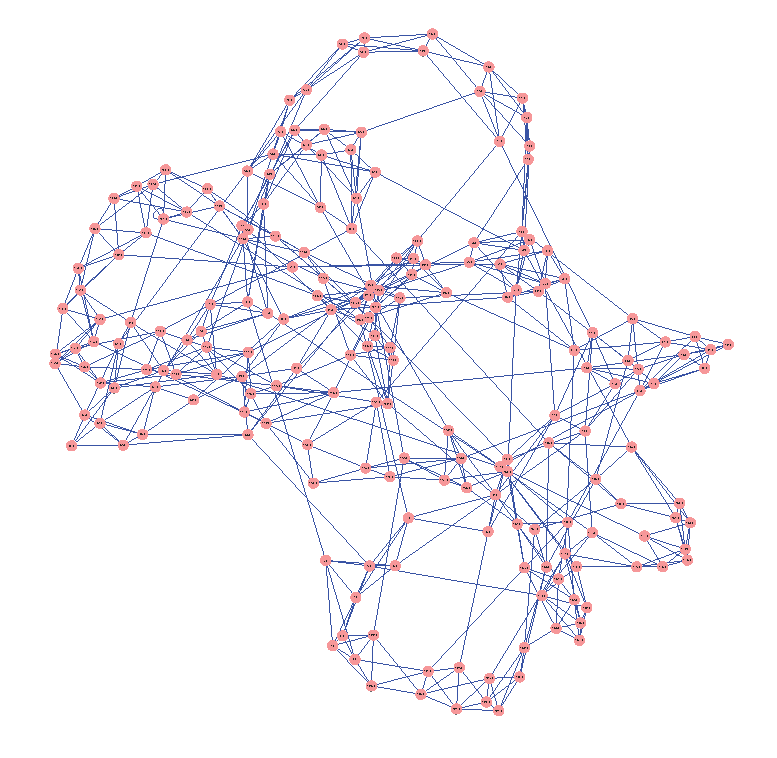
\includegraphics[width=3in]{introduction/wattsstrogatz.eps}
\caption{小世界网络.}\label{smallworld}
\end{minipage}~~
\begin{minipage}[t]{0.48\linewidth}
\centering
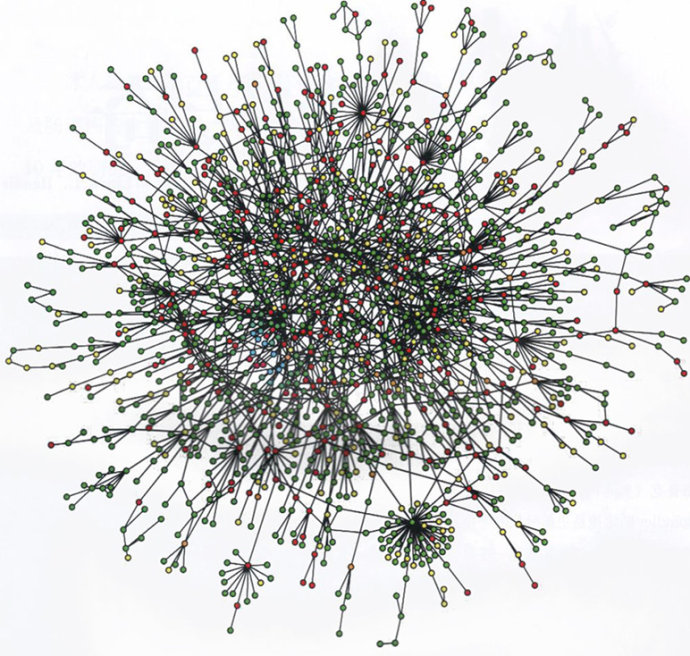
\includegraphics[width=3in]{introduction/scale.png}
\caption{无标度网络.}\label{scalefree}
\end{minipage}
\end{comment}

20世纪末, 科学家们发现, 很多网络都具有高度的集群性、不均衡的度分布以及中心节点结构. 这类结构的网络恰好是介于规则网络和随机网络之间, 但是它的统计特征与规则网络和随机网络截然不同. 国际上出现两项具有里程碑意义工作: 1998年, Watts和Strogatz在《自然》杂志上提出了介于规则网络和随机网络之间的新型网络——小世界网络\upcite{2}(如图 \ref{smallworld}). 小世界网络是在规则网络的基础上以一定的概率断开连边后在重新随机连接其他的节点所形成的网络. 当切断连边的概率取$0$、$1$ 两个极端值的时候, 此时小世界网络分别就是变成规则网络和随机网络(如). 生活中的很多网络都表现出小世界特性, 例如蛋白质分子相互作用网、手机通讯网络、科学引文网以及社会关系网等. 小世界网络的提出, 进一步证实了“六度分离”假说.

%在小世界网络出现之前, 人们认为网络分为完全规则网和完全随机网, 这两类网络具有各自的特征. 规则网络具有较大的特征路径长度, 聚类系数也较大, 而随机网络具有较小的特征路径长度, 但是聚类系数较小. 但现实中的网络如电网、交通网络、脑神经网络、社交网络、食物链等都表现出小世界特性, 即具有较高的聚类度和较小的特征路径长度. 也就是说小世界网络中大部份的节点彼此并不相连, 但绝大部份节点之间经过少数几步就可到达.
\begin{comment}[htb]
  \center
  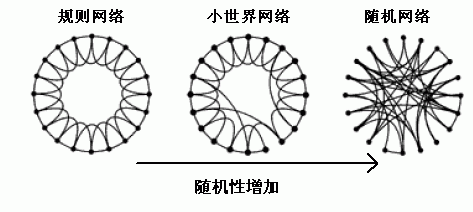
\includegraphics[width=3in]{introduction/smallnetwork.png}\\
  \caption{规则网络、小世界网络、随机网络之间的关系.}\label{SWN}
\end{comment}

一年后, Barabási等人于1999年在《科学》杂志上出了另外一种非均匀的网络模型——无标度网络\upcite{0}(如). 这类网络不仅拥有较大的聚类特性和较小的平均路径长度, 而且节点的度分布具有幂指数函数的规律. 许多复杂网络系统, 例如因特网路由关系网, 人力资源关系网等, 其网络中的大多数节点都是与某些特殊的节点有关联, 即网络中存在个别具有主要控制能力的节点. 这种网络节点间关系的不均匀性称为无标度网络的无标度性, 这种不均匀性是网络内在的一种性质.
复杂网络的“小世界”与“无标度”等统计特性的发现, 不仅丰富了网络内部结构的拓扑形式, 更进一步推动了研究者对复杂网络结构不断探索的热潮, 同时也加快了复杂网络理论在各个学科的研究进程\upcite{4,5,6,7,8,9,10}.


进入21世纪后, 小世界效应和无标度特性的提出使得复杂网络的理论研究蒸蒸日上, 并形成多学科交叉的理论成果. 近年来, 众多理论模型和分析方法如雨后春笋般涌现, 并且尝试利用复杂网络理论成果来解决各领域的实际问题. 目前主要研究工作分为: 一是研究网络内部耦合结构的变化以及统计特征, 例如网络系统的平均路径长度、聚集系数、度及度分布、谱性质、介数、小世界效应、无标度特性等特征; 二是研究复杂网络动力学行为, 包括鲁棒性、稳定性、一致性、以及同步问题等; 三是复杂网络在各个领域的应用, 包括生物医学、保密通信、图像处理、交通运输等领域\upcite{15,16,17}.


\section{复杂网络同步控制及其研究现状}
同步(synchronization)指的是两个或者两个以上性质相同或相似的动力系统通过系统节点之间的相互影响使得各个节点的动力学行为随着时间演变慢慢地趋于同一步调. 复杂网络的同步是一种群集行为. 自然界中同步现象数不胜数, 其中两个最为经典的同步现象是: 1665年, 荷兰物理学家、数学家惠更斯发现自家墙上的两个挂钟不论钟摆开始时如何摆动, 一段时间后, 两个摆钟的摆动频率完全相同, 摆动的方向恰好相反; 1680年, 荷兰旅行家肯普弗在旅行时注意到一个奇特的现象: 停留树枝上的萤火虫闪光的频率非常有规律, 几乎都是同时闪或者不闪. 除此之外, 生活中还存在各式各样的同步现象, 例如鱼群朝同一方向游动, 大雁群的一致飞行, 演唱会观众的拍手声等等.

1990年Pecora和Carroll\upcite{10}发现一类混沌系统的同步现象, 从此拉开了同步理论的研究序幕. 随着科学家们的不断深入研究, 目前已经出现了各种不同形式的同步模式:
有限时间同步\upcite{finitetimesyn}、固定时间同步\upcite{fixsyn}、 完全同步\upcite{abssyn}、 簇同步\upcite{clusyn}、位相同步\upcite{phasyn}、指数同步\upcite{23}. 其中, 完全同步指的是只需要当时间趋于无穷时, 网络所有的节点之间的误差趋于零, 它是同步模式中最普遍的一种. 而指数同步是指误差以指数形式趋于零, 它是比完全同步具有更快同步速度的同步模式. 本文仅讨论这两种同步模式.

在近十多年里, 人们对各种复杂网络拓扑模型的同步问题进行了广泛地研究并积累了大量的研究成果\upcite{Karimi5,Multi6,Lu7,Liu8,Karimi10,Lu9,Turci11,Jin12,Turci13}. %2014 年Wang和Tang等人\upcite{p30,p31}对近十年来复杂网络的研究成果进行了概括总结, 并指出未来复杂网络研究的挑战.
但大多数的研究成果都是基于理想的假设: 网络所处的环境是保持不变的, 即网络的耦合结构、耦合强度是固定的, 且网络节点间的通讯不会受到其他外在因素的干扰. 然而, 在实际问题中, 这个假定很难被认为是合理的. 事实上, 在现实应用中, 网络系统的节点状态、耦合结构和耦合强度不可避免地遭受来自外部随机因素的干扰.
例如电力输送网会受到地震、火灾、雷击、输变电系统短路等不可预知因素的影响; 保密通讯会受到黑客的攻击等等.
因此考虑随机环境下的网络同步更加具有实际意义.
最近几年, 研究者们开始重视对随机环境下复杂网络的同步问题的研究, 并且现在成为了一个较为活跃的研究方向. 随机环境下复杂网络同步问题研究的主题包括: 一是运用连续时间马尔可夫链来模拟复杂网络耦合结构随随机环境切换的变化过程\upcite{Li15,p10Markovian,p11Markovian,mm19,M20,M21,M22,M23,M24,M25,M17}; 二是引入随机变量来刻画耦合强度的随机性以及随机发生的耦合关系\upcite{X18,M19,randomcoupling1}; 三是通过布朗运动来模拟随机噪声对网络节点自身以及节点之间信号传输过程的干扰\upcite{Eventmultiagentnoises,p29,p30,p31,p32}. 尽管随机环境下复杂网络同步问题的研究取得较大的进展, 但还有许多问题亟待解决.
例如, 节点间状态信息的传输并非是简单的线性可观测形式, 而是通过非线性映射后的形式; 信息传输的有限速度和带宽引起网络节点自身动力学时滞的问题, 马尔可夫链转移率获取困难而引起的部分未知转移率的切换拓扑同步问题, 等等. 这些问题的解决能够更进一步完善复杂网络同步理论.

在现实生活中, 网络很难依靠自身节点之间的拓扑关联实现同步(自然同步)\upcite{phasyn,natsyn}. 这是由于网络内部节点庞大, 节点间的关联较为稀疏, 并且网络节点的关系会遭受到外部随机因素的干扰. 因此, 需要对网络施加外力, 即引进控制输入, 来促使网络实现的同步.
随着理论研究的深入, 很多控制策略被提出. 比较经典而且经济的控制策略是牵制控制\upcite{pin1,pin2,pin3}. 它只需要控制系统中极少数重要的节点, 然后通过节点的耦合关系将控制输入信号传送到其他的节点, 从而使得整个网络在控制节点的带领下达到同步状态. 相对于全局控制, 牵制控制具有可操作性强且节省控制成本的优势.
不过, 全局控制或者牵制控制都是采取连续通信模式, 系统连续不断地更新自身信息状态和控制输入信号, 并且实时地向邻居节点发送当前状态信息. 显然, 这种模式会导致不必要的带宽和能源消耗, 加大了网络的通讯负荷, 并且降低了网络抗干扰能力.

随后, 研究者们提出了数据采样机制来降低降低节点间的通讯以及控制输入的更新, 数据采样机制主要有周期采样\upcite{period}以及事件激发采样. 根据周期选取的不同, 周期采样又分为固定周期采、时变周期采样、以及随机周期采样. 相对于连续通信模式, 周期采样以一定的频率进行采样并更新节点状态和控制项, 一定程度上节省了控制成本, 并且减少了节点间的通讯频率. 尽管周期采样模式能够减小能量的消耗和降低网络的通讯负荷, 但是该通讯模式对周期的选择较为敏感, 若周期过短会导致较大的计算负荷, 若周期过长会导致同步速度较慢. 另外网络不能够根据自身的状态自适应地调整采样的频率. 不同于周期采样, 事件激发采样机制能够根据网络自身节点间的关系以及节点与同步目标之间的误差来决定采样时刻, 即系统能够自身的运行状况自适应地调整采样周期, 事件激发采样机制正好弥补了周期采样在周期选择上的缺陷. 事件激发采样控制策略被广泛应用于多主体系统一致性控制问题\upcite{Eventmultiagentnoises,eventmult2,eventmult3,eventmult4,eventmult5,eventmult6,eventmult7,eventmult8,eventmult9}, 最近有研究者开始关注事件激发采样控制策略在复杂网络同步问题中研究, 并取得了一些进展性工作\upcite{eventsyn1,eventsyn2,eventsyn3,eventsyn4,eventsyn5,eventsyn6,eventsyn7}. 事件激发采样模式的主要思想是: 当系统节点与同步目标之间的偏差大于给定的阈值时, 即此时事件被触发, 节点就更新自身的状态和控制项, 并向邻居节点传递信息. 换句话说, 网络节点的信息更新和信号的传输只发生在事件激发时刻. 事件激发采样控制模式最大的特点是网络根据节点自身的状态按照需要进行更新和传递数据信号, 从而能够极大减少通信的频率, 节省能量. 正如K. {\AA}ström\upcite{eventsyn8} 和B. Wang\upcite{eventsyn9}等人证实, 事件激发采样控制策略比周期采样策略表现出更好性能.

事件激发采样策略的核心在于根据网络节点间的关系定义激发规则. 按照监控时间是否连续可以分为连续监控激发规则\upcite{eventsyn5}和离散监控激发规则\upcite{eventsyn7}; 按照激发时刻是否一致可以分为集中式激发规则\upcite{Eventmultiagentnoises}和分散式激发规则\upcite{eventmult3}. 连续监控激发规则不仅依赖于节点及其邻居最新激发时刻状态信息, 而且依赖于节点当前的状态信息, 即需要对节点的状态进行实时的监控. 而离散监控激发规则只需根据最新激发时刻的状态信息对下一次激发时刻进行预测, 在下一次激发到来之前, 节点的状态不需要进行监控. 这两种激发规则各有利弊, 连续监控激发规则花费较大的监控成本, 但是激发频率较低, 从而降低了网络间的通讯负荷, 更有利于网络的稳定; 而离散监控激发规则监控成本较低, 但会增加激发频率, 加大通讯负荷. 在实际应用中一般根据监控成本和通讯负荷来衡量运用那种激发规则. 集中式激发规则要求所有节点的激发时刻一致, 即根据网络节点的信息状态对每个节点定义统一的激发规则. 而分散式激发规则每个节点根据自身状态和邻居最新的更新信息定义自己的事件触发规则. 相比较而言, 集中式采样策略具有更低的计算负荷, 并且能更快地促使系统达到同步, 但激发频率比分散式采样策略要高.

目前, 利用事件激发采样策略研究复杂网络问题还处于起步阶段, 主要集中在以下几个方面: 一是通过有限时间事件激发研究带马氏链的非线性系统鲁棒性的问题\upcite{eventnonlinear}; 二是利用事件激发通讯协议研究带马尔可夫跳网络的状态估计问题\upcite{eventMarkov4, eventdelay3}; 三是设计事件激发策略研究多主体系统一致性问题\upcite{consensus1,consensus2}; 四是基于事件激发采样控制策略研究一般马氏切换拓扑复杂网络的同步问题\upcite{eventMarkov3,eventMarkov0,eventMarkov2}; 五是采用事件激发采样协议研究转移率未知的马氏跳复杂网络的控制问题\upcite{eventdelay1,eventunknown}. 尽管事件激发采样技术在网络研究方面已有相关的理论成果, 但为数不多. 特别是在复杂网络的同步问题上, 一方面, Liu、Shao、Wang等人\upcite{eventMarkov3,eventMarkov0,eventMarkov2}所考虑的都是简单的线性耦合系统, 同时也未考虑到耦合关系随机中断、耦合强度随机变化的情况, 除此之外, 他们也没有在离散监控的情形下设计事件激发采样策略. 另一方面, 对于转移率未知的问题, Senan\upcite{eventdelay1}讨论了带混合时滞的转移率未知的带马氏跳神经网络的同步问题, Li\upcite{eventunknown}给出了转移率未知的马氏跳网络随机稳定性的充分条件, 并给出了事件激发的上界, 证实了Zeno现象不会发生. 然而, 对于部分转移率未知、动态同步目标以及时滞共存的复杂网络同步问题并未发现相关成果, 此外对于节点状态信息在传输过程中受到噪声干扰的模型也未见有研究者们利用事件激发采样技术来给出同步判据. 这些网络模型同步问题的解决, 能够更一步地完善事件激发采样策略下复杂网卡控制同步问题的理论. 本文将逐一讨论运用事件激发采样控制去研究这类带有随机因素影响的复杂网络同步问题.

%
%例如, Li等人\upcite{eventsyn1}应用事件激发策略与间歇通讯策略相结合研究了动态复杂网络的同步问题; Chen 等人\upcite{eventsyn2}分别设置连续监控激发规则和离散监控激发规则研究线性耦合复杂网络的同步问题; Lu等人\upcite{eventsyn7} 通过事件激发策略与牵制控制方法得出了带马尔科夫切换线性耦合复杂网络的同步判据; Lang等人\upcite{eventsyn5}基于事件触发策略研究了带迟滞的神经网络的同步问题; Guinaldo 等人\upcite{packetloss} 通过事件触发策略研究了带迟滞和数据包丢失的复杂网络的同步问题. 尽管事件激发控制策略在同步问题上得到了较好的应用, 但仍然有一些问题有待解决. 上述成果很少有考虑到随机环境对系统的影响. 特别是噪声对信号传输过程的干扰以及控制器偶然失败的情况. 除此之外, 马尔可夫调制的耦合结构在状态切换时的转移概率并非完全已知, 并且非线性的耦合方式更是具有挑战性. 本文将讨论运用事件激发控制去研究这类复杂网络的同步问题.


\section{本文的主要工作及创新点}

本文主要利用事件激发策略控制方法研究了几类带有马尔可夫切换的复杂网络同步问题. 通过设定合适的事件激发规则, 基于Lyapunov稳定性理论、矩阵理论、随机过程理论等知识推导出几类马尔可夫切换网络的同步判据, 并给出数值仿真例子证实理论结果的有效性.

本文工作分为六个章节, 其各个章节工作内容如下:

第一章介绍复杂网络及其同步的研究背景和意义, 简单概述和分析国内外有关复杂网络同步研究的现状, 并介绍复杂网络常用控制方法以及基于事件激发控制策略的优点, 最后简要叙述本文工作及创新点.

第二章给出复杂网络的理论和模型, 介绍随机过程理论的基础知识, 最后给出复杂网络同步的数学定义、证明主要结论所有的引理、及本文所用的记号.

第三章对非线性随机发生耦合的复杂网络同步问题进行了研究. 网络模型是在卢文联2015年研究的一篇文章\upcite{eventsyn2}基础上进行改进, 模型不仅包含了马氏切换和非线性耦合, 而且也考虑了网络节点间的耦合关系和耦合强度受到随机因素影响的情形, 即随机发生的耦合和随机耦合强度. 基于分散式事件激发控制策略下, 分别给出连续监控形式的同步误差上界(CRS) 和指数函数上界(CRE) 激发规则以及离散监控情形下的同步误差上界(DRS)和指数函数上界(DRE)激发规则. 利用稳定性理论、随机过程理论、以及矩阵分析理论推导出同步的充分条件. 最后, 对于四种不同激发策略, 分别比较其优缺点和适用场景. 并给出一个数值仿真来验证本节结论的有效性.

第四章基于集中式事件激发策略研究了部分转移率未知时滞的复杂网络同步问题. 本章在第三章的基础上进行拓展, 在马氏切换拓扑的基础上, 对部分转移率未知以及节点自身动力学存在时滞的网络进行研究. 基于集中式事件激发策略, 设计随机发生的控制器来驱使网络达到同步. 在稳定性理论、随机过程理论、以及矩阵分析理论下证实给出的同步判据是充分有效的. 同时, 也给出了几个一般模型下的推论. 最后给出事件激发间隔的下界, 从而证实Zeno现象不会发生. 数值仿真揭示理论结果的有效性. 本章的主要结果已发表在Applied Mathematics and Computation杂志.

%由于网络带宽有限, 信号的传输可能会发生延迟, 因此考虑迟滞的复杂网络模型更加符合实际.
%除了系统上的改进外, 在目标节点的选择上也做了改进. 前两章主要考虑的是已知同步目标, 也就是说网络同步目标$s(t)$是根据孤立节点动力学$s(t)=\dot{f}(s(t))$确定的, 这在有些场合并不适合. 例如, 在讨论会上我们并没有提前讨论的结果, 讨论的结果是通过讨论者的观点不断影响他人, 最后大家形成一致的意见或者得出同一的解决方案. 因此研究动态同步目标也是有必要的. 另外, 本节还给出了事件激发区间的下界, 从而避免了Zeno现象. 最后

第五章研究部分转移概率未知带噪声干扰的复杂网络同步问题. 通过引进布朗运动模拟网络节点间信号传输过程中噪声的影响, 分别在集中式和分散式事件激发策略下, 构造马氏调制的线性控制器. 然后利用伊藤公式、Lyapunov 稳定性定理等知识, 给出部分转移概率未知且带随机扰动马尔可夫网络的同步判据. 最后通过实验仿真证实定理给出的判定条件的有效性, 并分析噪声对网络同步性能的影响.

%前两章主要分析了非线性和时滞模型, 考虑马尔可夫链的转移率是部分未知以及带噪声扰动的情形. 因为耦合关系的切换有时候并不完全知道切换的概率, 同时网络节点之间的信息传输会受到噪声的干扰, 从而导致网络的不稳定性. 所以本节主要研究部分未知转移率且带有噪声的马尔可夫网络.

第六章总结论文的主要工作, 并给出本文存在的不足之处, 最后指出今后可能的研究方向.

本文的主要创新点如下:

\begin{itemize}\setlength{\itemsep}{0cm}
  \item 线性耦合结构的复杂网络同步问题已经得到广泛研究, 并且具有较丰富的理论结果. 非线性耦合尽管有一些成果, 但也都是建立在连续采样或者周期采样的模式下, 这在一定程度上会加大网络节点间的通讯负荷. 目前基于事件激发策略的控制方法研究非线性耦合关系马氏切换网络的理论结果还未有人提及. 本文在线性基础上, 研究了随机发生的非线性耦合、随机耦合强度以及事件激发控制模式共存的网络模型同步问题;
  \item 在网络耦合关系随机性方面, 本文不仅考虑马氏切换去模拟随机的切换的拓扑, 还考虑耦合关系在切换过程中的转移率是部分未知. 除此之外, 网络节点存在迟滞的情况也加入到模型中, 同时引进动态的同步目标. 设置合适的事件激发策略控制网络达到同步;
  \item 针对部分转移概率未知迟滞的网络模型, 给出事件激发区间的下界, 证实了Zeno现象不会发生;
  \item 噪声是一项不可避免的随机因素, 而噪声一般对网络节点自身和网络节点间通讯都会造成影响. 相对于网络节点自身, 通讯干扰对网络稳定性影响更大. 很多研究者往往只考虑了节点自身动力学行为受到噪声扰动, 而本文在离散通讯模式下加入布朗运动模拟节点间的信号传输过程中受到噪声扰动.
\end{itemize}


%%!Mode:: "Tex:UTF-8"
\chapter{预备知识}\label{chap:math}
\section{复杂网络的理论和模型}
        网络是一类描述自然系统和人工系统的模型. 一个网络是具有一定特定功能群体. 其中每个个体都具有自己的动力学行为, 而个体间存在着相互的联系和影响. 这种联系和影响可以利用图论来描述: 网络的个体可以看作图的节点, 个体之间的联系和影响可以用图的边来表示. 网络节点的状态不仅取决于自身动力学的特性, 而且受到与之有联系节点的影响.
        复杂网络是具有大规模节点和复杂的连接拓扑结构的网络. 其复杂性主要体现在两个方面, 一是节点的动力学行为, 它既可以是线性有序的动力学行为, 也可以是非线性或者时空混沌动力学行为; 二是复杂的拓扑结构, 主要体现为时滞拓扑、切换拓扑、时变拓扑、以及噪声干扰的拓扑相混合而成的拓扑结构.

        一个由$N$个$n$维状态恒同节点组成的线性耦合复杂网络模型为:
        \begin{comment}
           \dot{x}_{i}(t)=f(t,x_{i}(t))-c\sum^N_{j=1}l_{ij}\Gamma[x_{j}(t)-x_{i}(t)], \quad i = 1,\cdots,N,
        \end{comment}
        其中是第个节点在时刻的维状态向量; 连续映射是节点自身动力学特性; 是网络的耦合矩阵, 其中表示节点与节点之间的影响权重, 如果点与节点 有关联, 即网络拓扑图存在边, 则, 否则, 其中,  是网络节点间的耦合强度; diag是内耦合矩阵, 描述节点个状态之间的相互作用.

        在现实生活中, 很多网络系统通过自身节点间的调节很难达到同步. 因此需要人为地加入适当的控制. 此外网络系统的耦合关系常常会因所处环境的变化而变化. 本文主要利用事件激发采样控制方法研究带有切换拓扑的复杂网络同步问题. 一般的网络模型如下:
        \begin{comment}\label{eventcontrolnetwork}
           \nonumber \dot{x}_{i}(t)&=f(t,x_{i}(t))-c\sum^N_{j=1}l_{ij}(r_{t})\Gamma[x_{j}(t_k)-x_{i}(t_{k})]+u_i(t),\\
            &\quad\quad t_{k}\leq t< t_{k+1}, \quad i = 1,\cdots,N,
        \end{comment}
        其中是有限状态空间齐次马尔可夫链; 是严格递增的事件激发时刻序列; 是网络控制输入.
        \begin{defn}\label{defn1}%\upcite{nonl-asym}
            如果一个网络系统对于任何的初始值, 以及任意两个节点满足\

            则称该网络系统在均方意义下能够达到同步, 简称\textbf{均方同步};
            如果存在两个正数和, 使得

            则称该网络系统在均方意义下能够达到指数同步, 简称\textbf{均方指数同步}.
        \end{defn}
    \begin{rem}
    从 可以看出, 均方指数同步是网络中任意两个节点的所有状态向量之差的范数平方的期望指数递减于零, 它是均方同步的一种特殊情况.
    \end{rem}
\section{随机过程理论}
    随机过程(Stochastic Process)是有限维随机变量的推广, 它是无穷多个随机变量形成的随机变量序列, 是概率空间上的一族随机变量. 自协方差只与时间差有关的随机过程称为平稳过程. 任意增量都相互独立的随机过程称为独立增量过程. 常见的随机过程有泊松过程、更新过程、马尔科夫过程、鞅、以及布朗运动. 本文主要利用随机过程论中的马尔可夫链和布朗运动相关理论去研究复杂网络的微分动力学系统.

    {\bf 马尔可夫过程:} 具有无后效性或者马氏性的随机过程称为马尔可夫过车. 即将来的发展状态只与当前的状态有关, 而与过去的状态无关的随机过程. 在现实生活中, 有很多过程都是马尔可夫过程, 如液体中微粒所作的布朗运动、传染病受感染的人数、车站的候车人数等, 都可视为马尔可夫过程. 在复杂网络研究中可以用马尔可夫过程来描述网络系统处于不同外在环境时耦合结构的切换过程. 下面该过程的数学定义:
    \begin{defn}\upcite{stoprocc}
           设状态空间, 随机过程对于任意, , , 若, 就有
           \begin{comment}
                P\{r(t_{n+1})=i_{n+1}|r(t_0)=i_0,r(t_1)=i_1,\cdots,r(t_n)=i_n\}=P\{r(t_{n+1})=i_{n+1}|r(t_n)=i_n\}
            \end{comment}
            则称为连续参数马尔可夫链(简称连续参数马氏链). 若对于任意, 有
            \begin{comment}
                P\{r(s+t)=j|r(s)=i\}=P\{r(t)=j|r(0)=i\}=p_{ij}(t).
            \end{comment}
            则称为齐次马尔可夫链, 称为转移概率矩阵. 本文仅考虑有限状态空间的齐次马尔可夫链.
    \end{defn}
    \begin{lem}{\rm\upcite{stoprocc}}
            当为有限状态空间时, , 极限
            \begin{comment}
                q_{ii}\triangleq\lim_{t\rightarrow0}\frac{1-p_{ii}(t)}{t},\quad q_{ij}\triangleq p'_{ij}(0)=\lim_{t\rightarrow0}\frac{p_{ij}(t)}{t}.
            \end{comment}
            存在且有限, 并且有. 称为的转移率矩阵, 或称密度矩阵.
    \end{lem}

    部分未知转移率的马尔可夫链的转移矩阵具有如下形式:

        这里代表未知的转移率. 为了记号上方便, 对任意, 记, 其中, .

    {\bf 布朗运动:} 是指空气或者液体中的微粒受到气体或者液体的原子或者分子的碰撞而产生的一种无规则的随机运动. 最先发现这种无规律的运动是英国植物学家R.布朗, 他在做植物实验时候发现水中的花粉颗粒不停地无规律运动, 即使过再长的时间, 这种无规律的运动也不会停止. 后来他进一步实验证明, 不仅花粉微粒, 任何微小粒子在空气中或者是在流体中都会表现出这种无规则运动. 后来人们把这种现象称之为布朗运动. 下面给出布朗运动严格的数学定义:
    \begin{defn}\upcite{stoprocc}
          设随机过程满足:

          (1) 是独立增量过程;

          (2) , 即是期望为, 方差为的正态分布;

          (3)  关于是连续函数.\\
          则称是布朗运动或维纳过程(Wiener process).
    \end{defn}
当时, 称是标准布朗运动, 此时若, 则.
    \begin{defn}[伊藤过程]{\rm\upcite{yitengprocc}}\label{yitengdefn}
          设是布朗运动, 是相应的域流. 伊藤过程是如下形式的随机过程:

          其中非随机, 是适应的随机过程.
    \end{defn}
    \begin{lem}[伊藤—德布林公式]{\rm\upcite{yitengprocc}}\label{yitformula}
           设是定义 中描述的伊藤过程, 函数的偏导数, 和都有定义并且连续, 则对于每一个, 有:
            \begin{comment}
                f(T,X(T))&=f(0,X(0))+\int_0^Tf_t(t,X(t))dt+\int_0^Tf_x(t,X(t))\Delta(t)dW(t)\\
                &\quad+\int_0^Tf_x(t,X(t))\Theta(t)dt+\frac{1}{2}\int_0^Tf_{xx}(t,X(t))\Delta^2(t)dt.
            \end{comment}
    \end{lem}
    \begin{rem}
         是以精确的数学语言叙述的. 公式右端每一项都有确切的含义, 第一项是非随机, 第三项是一个伊藤积分之和, 其余三项是关于时间变量的勒贝格积分.
    \end{rem}
    将上述伊藤—德布林公式写成微分形式记法如下:
    \begin{comment}
                df(t,X(t))&=f_t(t,X(t))dt+f_x(t,X(t))\Delta(t)dW(t)\\
                &\quad+f_x(t,X(t))\Theta(t)dt+\frac{1}{2}f_{xx}(t,X(t))\Delta^2(t)dt.
    \end{comment}

\section{相关定义、引理}
    {\bf 符合说明:} 如果没有特殊说明, 则在文中表示阶单位矩阵, 表示具有适当维数的零矩阵; 是阶矩阵 的特征根, 若所有的特征根均为实数, 不妨将其排序为: ; 记作向量的转置,  记作向量 欧几里得范数; 记作元素全部是的 维向量; 符号表示数学期望, 符号表示Kronecker积.
    \begin{defn}\upcite{clusyn}\label{quad}
        称函数满足条件, 记作, 如果存在两个正定对角阵, 和一个正数, 使得对任意, 有

    \end{defn}
    \begin{defn}\label{lipuxici}
        称函数属于函数类, 记作, 如果存在两个正数和, 使得对任意, 有
        \begin{comment}
            \| f(x)-f(y)\|\leq l_{1}\| x-y\|,\\
            \| f(x)+f(y)\|\leq l_{2}\| x+y\|.
        \end{comment}
        称函数属于函数类, 记作, 如果存在非零常数, 使得对任意, 有
        \begin{comment}
            (x-y)^\top(g(x)-g(y))\geq \sigma(x-y)^\top(x-y).
        \end{comment}
    \end{defn}
    事实上, 现实存在的很多混沌系统, 比如洛伦兹系统, 陈氏系统, L 系统和 Chua's 电路系统, 他们的自身动力学函数都满足 和.
    \begin{lem}\label{lem:1}{\rm\upcite{Kronecker}}
        设和是具有合适维数的矩阵, 则下面性质成立:
        \begin{comment}
            \left\{
            \begin{commented}
            &(aA)\otimes B=A\otimes(aB);\\
            &(A+B)\otimes C=A\otimes C+B\otimes C;\\
            &(A\otimes B)(C\otimes D)=(AC)\otimes (BD);
            \end{commented}
            \right.
            \end{comment}
        其中是常数.
    \end{lem}
    \begin{lem}\label{lem:2}{\rm\upcite{Kronecker}}
        设矩阵, 是对称矩阵, 则对任意, 有
        \begin{comment}
            \lambda_{1}(A)\cdot\lambda_{1}(B)x^{\top}x\leq x^{\top}(A\otimes B)x\leq \lambda_{n}(A)\cdot\lambda_{m}(B)x^{\top}x.
        \end{comment}
    \end{lem}
    \begin{lem}{\rm\upcite{leq}}\label{lem_leq}
           设, 是维向量, 则对任意阶半正定矩阵以及任意常数, 有
            \begin{comment}
            2x^{\top}Py\leq\mu x^{\top}Px+\frac{1}{\mu}y^{\top}Py
            \end{comment}
    \end{lem}

    \begin{lem}[Lyapunov稳定性定理]\label{lem:lyapunov}
        设是非线性系统:
        \begin{comment}
          \dot{x}=f(x), \quad f(0)=0
        \end{comment}
        其中, 满足局部{\rm{Lipschitz}}条件
        的平衡点, 是包含原点的定义域. 设
        是连续可微的函数, 如果
        \begin{comment}
          &V(0)=0;\\
          &V(x)>0,\quad x \in D-\{0\};\\
          &\dot{V}(x) \leq 0,\quad x \in D;
        \end{comment}
        那么, 平衡点是稳定的. 特别的, 如果

         那么, 平衡点是渐近稳定的.
    \end{lem}
\begin{lem}[Lyapunov—Krasovskii稳定性定理]\label{lem:lyapunov}
考虑时滞微分方程
\begin{comment}
    \dot{x}(t)=f(t,x(t))
\end{comment}
这里是一个连续函数, 同时将的一个有界子集映射到一个的有界子集, 令是连续并且严格单调非减函数, 满足当为正, 同时有. 如果存在一个连续函数使得

和

成立, 这里是沿着上述时滞微分方程解的导数, 那么这个方程的解就是一致渐近稳定的. 这个函数被称之为{\rm{Lyapunov—Krasovskii}}函数.
\end{lem}
%%!Mode:: "Tex:UTF-8"
\chapter{分散式事件激发采样下带马氏切换的非线性随机耦合网络同步问题}\label{chapternonline}
    目前, 复杂网络同步问题已经得到研究者广泛研究. 早些时候的网络同步问题的理论成果主要是建立在固定耦合拓扑的假设之上, 即网络节点间的耦合关系只有一种模式. 后来有研究者发现, 在实际应用中网络节点间的关系并不是一成不变的. 例如在企业关系网中, 企业与企业之间某时期是竞争关系, 但在某时期会转为合作关系. 显然, 变化的拓扑结构更加适应于实际的网络模型. 研究者们提出, 通过引入马氏链来模拟网络拓扑结构在不同外环境中的切换过程. 本文在前人的基础上, 继续探讨具有马氏切换拓扑结构的复杂网络同步问题.
    节点间的线性耦合是较为简单的耦合方式, 对于大规模节点的网络, 节点间的耦合关系往往不能够直接观测得到, 而是观测到其经过非线性函数映射后的结果. 因此研究非线性耦合的结构更符合实际网络环境且更具有挑战性. 特别是在保密通讯方面, 线性的耦合结构比较容易受到黑客的攻击, 不利于通讯安全. 将信号通过非线性转换后再传输能够极大地提高了信息传输的安全性.

    很多现实中的网络很难达到同步或者同步时间较长, 因此需要引进控制方法促进网络快速到达同步. 控制方法根据采样时间是否连续可以分为连续采样控制和非连续采样控制, 其中非连续采样控制方法有周期间歇控制、脉冲控制、以及基于事件激发采样控制. 事件激发采样控制策略的基本思想是网络节点间的信息传输只发生在事件激发时刻, 而该时刻由只依赖于节点自身状态信息以及邻居节点上一次更新的状态信息的激发规则决定. 当激发规则满足时, 事件就会被激发, 此时采样行为发生, 相应的控制器发生更新. 基于事件激发采样不仅可以减少控制器的更新频率, 同时还可以减少节点间的通讯负荷. 根据节点是否具有一致的激发时刻, 可将事件激发采样分为分散式和集中式两种. 本章节采用的是分散式事件激发采样的控制策略去研究带有马氏切换非线性耦合复杂网络的同步问题.

    %在实际应用中, 由于系统可能会受到不可以预知的外在因素干扰, 复杂网络节点间的耦合关系并不是一成不变的, 节点与节点之间时而存在耦合关系, 时而中断耦合关系. 例如, 设备之间的通讯会受到电磁干扰、温度干扰、湿度干扰、声波干扰、振动干扰和射频辐射干扰等等, 从而会导致设备间的信号传输随时都有可能发生中断. 因此研究随机发生耦合复杂网络更具有实际应用. 目前, 有一部分研究者已经对随机发生耦合网络展开了相关的研究, 并取得了一些成果. 例如Yang\upcite{X18}和Baumeister\upcite{M19}等人分别研究了随机发生耦合神经网络的同步问题, 并给出了有效的同步判据. 然而这些作者一般考虑都是线性的耦合关系, 事实上, 网络节点之间的状态信息有时候很难观察到线性变量的值, 而只能观测到它的非线性函数的值. 故非线性耦合网络更有研究的必要. 除此之外, 很多现实中的网络很难到达同步或者同步时间耗时较长, 因此需要引进控制方法驱使网络快速到达同步\upcite{Lu9,Turci11,Jin12,Turci13,Li15,pwang30,ptang31,22,nonl-asym}. 尽管这些文献都提出了各种各样的控制方法, 但是它们都有一个共同的特点, 那就是控制都是实时更新的, 控制器频繁更新会加大能量损耗和通讯负荷. 理想的情况应该是根据网络系统的情况, 按照需要来更新控制器. 例如在军训时候, 教官为了使得学生的步伐达到同步, 会根据队伍的情况发出口令进行控制, 而不是教官一直不停地发出口令. 基于事件激发的控制策略正是解决控制器频繁更新的问题, 该策略是根据网络系统节点间关系、以及节点自身与同步目标之间的关系构造一个激发规则, 当激发规则满足时, 事件就会被激发, 相应的控制器发生更新. 这不仅可以减少控制器的更新频率, 同时可以见到节点间的通讯负荷. 本文就是利用事件激发的策略研究带有马氏切换非线性耦合复杂网络同步的问题.

\section{分散式事件激发采样的网络模型}\label{csnp:sec:moper}
        分散式事件激发采样的特点是每个节点都有自己的激发规则, 某节点的激发并不会引起其他邻居节点的激发, 但会将该激发时刻的采样信息转告给邻居节点使其更新激发规则. 本章节利用基于分散式事件激发采样的牵制控制方法研究带有马氏切换的随机发生非线性耦合复杂网络同步问题. 网络的随机性不仅体现在耦合模式是随机切换的, 同时还体现在随机发生的耦合以及随机耦合强度. 其网络模型如下:
        %在网络控制理论中, 根据控制节点的数量可以将控制方法分为全局控制和牵制控制(局部控制). 牵制控制主要思想是通过控制较少的节点, 然后通过网络节点间的联系来传输控制信号以实现网络同步. 相比于全局控制, 牵制控制能够节省控制成本. 有时候只需控制一个节点就可以实现了网络同步. 一般在控制节点的选择上偏向于具有较大度的节点. 本节将牵制控制方法和事件激发策略相结合, 研究带有马氏切换的随机发生非线性耦合复杂网络同步问题. 网络模型如下:
        \begin{comment}\label{sys:init1}
        \nonumber\dot{x}_{i}(t)&=f(x_{i}(t))-\theta(t)\rho(t)\sum^N_{j=1}l_{ij}(r_{t})\Gamma[h(x_{j}(t_{k}^{i}))-h(x_{i}(t_{k}^{i}))]+u_i(t), \\
        &\quad t_{k}^i\leq t< t_{k+1}^i, i = 1,\cdots,N,
        \end{comment}
        其中是伯努利随机变量, 满足, 它描述网络系统随机发生的耦合;
        是随机耦合强度, 其. 这里假设和是相互独立的;  是非线性耦合函数;
        是第个节点第次事件激发的时刻.
        控制输入的定义如下:
        \begin{comment}\label{nonlinearcontrol}
            u_i(t)=-\tau \rho(t)d_{i}(r_{t})\Gamma[h(x_{i}(t_{k}^{i}))-h(s(t_{k}^{i}))],
        \end{comment}
        这里是控制增益; 是牵制节点集上的示性函数, 即, 如果, 则, 否则;  是孤立节点动力学的轨道, 即同步的目标轨道.
        \begin{rem}
            该模型与  的不同之处是增加了非线性耦合、随机发生的耦合、以及随机耦合强度. 它更加符合实际生活中的系统, 具有更广泛的应用价值.
        \end{rem}

\section{分散式事件激发采样的复杂网络同步分析}
    本节主要探索在连续时间监控和离散时间监控下, 网络系统  能够达到同步的条件. 通过构造合适的事件激发规则, 结合稳定性理论, 推导出在两种情形下的同步判据. 在给出结论之前, 先给出必要的引理.
    \begin{lem}\label{lem:5}
            设矩阵满足, , 则对任意向量, , 有

    \end{lem}
    \begin{lem}[Gronwall—Bellman不等式]\label{lem:6}{\rm\upcite{Gronwall,Bellman}}
        设是区间上的连续函数.

       情形 如果在区间上非负可微, 且对任意, 有

       那么


       情形 如果在区间上非负可积, 且对任意, 有

         那么

    \end{lem}
    由于非线性耦合的结构形式众多, 并且及其复杂, 这里我们仅讨论符合以下假设的非线性函数类.
    \begin{hyp}\label{ass}
        假设存在正数, , 使得对任意, 有

    \end{hyp}
    \begin{rem}
        假设 \ref{ass} 是比较常见的, 只要函数满足一阶导数有界并且导数值为正数即可, 例如反正切函数就可以满足.
    \end{rem}
    记为节点的同步误差. 为了讨论方便, 引入下述记号:
        %\begin{flcomment}
        %\begin{split}
        \begin{eqnarray*}
        &&f(e_{i}(t))=f(x_{i}(t))-f(s(t)),\\
        &&h(e_{i}(t))=h(x_{i}(t))-h(s(t)),\\
        &&e(t)=(e^\top_{1}(t),e^\top_{2}(t),\cdots,e^\top_{N}(t)^\top),\\
        &&f(e(t))=(f^\top(e_{1}(t)),f^\top(e_{2}(t)),\cdots,f^\top(e_{N}(t))^\top),\\
        &&h(e(t))=(h^\top(e_{1}(t)),h^\top(e_{2}(t)),\cdots,h^\top(e_{N}(t)))^\top,\\
        &&D(r_{t})=\text{diag}\{d_{1}(r_{t}),d_{2}(r_{t}),\cdots,d_{N}(r_{t})\}.
        %\end{split}&
        %\end{flcomment}
        \end{eqnarray*}
       于是网络系统  可以写成误差系统的形式:
        \begin{comment}\label{sys:all}
        \dot{e}(t)=f(e(t))-\theta(t)\rho(t)[L(r_{t})\otimes\Gamma]h(e(t))-\tau \rho(t)[D(r_{t})\otimes\Gamma] h(e(t))+\rho(t)\tilde{e}(t),
        \end{comment}
       其中是系统测量误差, 其分量定义为如下:
        \begin{comment}
        \nonumber \tilde{e}_{i}(t)=&\theta(t)\sum^{N}_{j=1}l_{ij}(r_{t})\Gamma[h(x_{j}(t))-h(x_{j}(t_{k}^{i}))]\\
        &-\tau d_{i}(r_{t})[h(x_{i}(t))-h(x_{i}(t_{k}^{i}))+h(s(t_{k}^{i}))-h(s(t))].
        \end{comment}
\subsection{连续监控激发规则}
    在连续监控情形下, 监控器实时地收集节点和的状态信息, 事件激发规则根据收集到的节点状态信息判断此时是否满足激发条件. 如果关于某个节点 的激发规则满足, 则关于节点的事件就被激发, 从而获得新的事件激发时刻. 与此同时, 节点更新自身状态和控制器状态, 并且发送时刻的状态信息给邻居节点, 这里argmax. 于是邻居节点更新时的状态信息为 时的状态信息, 但关于邻居节点的事件不会被激发直到属于邻居节点的激发条件满足. 具体流程见.
    \begin{comment}[!htp]
    \setlength{\abovecaptionskip}{-1cm}
     \begin{center}
           {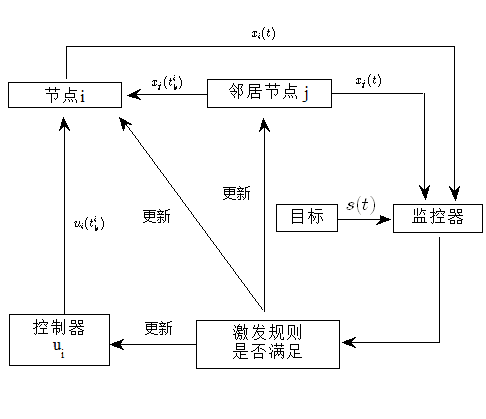
\includegraphics[width=4.5in]{nonlinear/flowchartcon1.png}}
     \end{center}
  \caption{连续监控下事件激发牵制控制流程图}\label{cflowchart}
    \end{comment}

    下面给出两种不同误差上界的激发规则:

           情形a: 基于同步误差上界的连续监控事件激发规则(简称为CRS激发规则):
            \begin{comment}\label{crule:1}
            t^{i}_{k+1}=\max\left\{t\geq t^{i}_{k}: \|\tilde{e}_{i}(t)\| \leq\omega \| e_{i}(t)\|\right\}
            \end{comment}

            情形b: 基于指数函数上界的连续监控事件激发规则(简称为CRE激发规则):
            \begin{comment}\label{crule:2}
             t^{i}_{k+1}=\max\left\{t\geq t^{i}_{k}: \|\tilde{e}_{i}(t)\| \leq ae^{-bt}\right\}
             \end{comment}
           其中, , , ,
              , .

            网络系统激发的具体算法如下:
            \begin{algo}[连续监控事件激发算法]\label{algo1}~~

             对, 初始化:

             当时, 监控器实时收集节点, 的状态信息并发送到激发机制 或者

             若果或者 , 则事件被激发, 最新的激发时刻, 则返回;

             当时, 节点以及它的邻居节点和控制器将会更新状态信息, 即用时刻状态信息替换时刻的状态信息, 返回.
             \end{algo}

        下面给出连续监控情形下的同步判定定理.
        \begin{thm}\label{themcon}
            如果假设  成立, 属于, 并且存在正定对角阵, , 使得对任意, 有
            \begin{comment}\label{thm:1}
            \bar{\delta}P(u)\otimes G-c\theta\underline{\alpha} P(u)L(u)\otimes G\Gamma
            -c\tau\underline{\alpha} P(u)D(u)\otimes G\Gamma+\frac{1}{2}\sum_{v=1}^{m}q_{uv}P(v)\otimes G\leq 0,
            \end{comment}
            其中, .
            那么, 基于激发规则或者激发规则, 按照算法 , 网络系统  可以实现均方指数同步.
        \end{thm}
        \begin{proof}
        在时, 定义随机Lyapunov—Krasovskii函数如下:
        \begin{comment}
            V(t)=\frac{1}{2}e^{\top}(t)[P(u)\otimes G]e(t).
        \end{comment}
        记是弱无穷小生成元算子. 根据 和式  以及条件, 有
            \begin{comment}\label{diff:V}
            \nonumber \mathrm{E}\mathcal{L}V(t)&=\mathrm{E}\bigg\{e^{\top}(t)[P(u)\otimes G]\Big [F(e(t))-I\otimes\Delta e(t)+I\otimes\Delta e(t)-c\theta \left[L(u)\otimes\Gamma\right] H(e(t))\\
            \nonumber &\quad-c\tau[D(u)\otimes\Gamma] H(e(t))+c\tilde{e}(t)\Big]+\frac{1}{2}\sum_{v}q_{uv}e^\top(t)\left[P(v)\otimes G\right]e(t)\bigg\}\\
            \nonumber &\leq \mathrm{E}\bigg\{(\bar{\delta}-\xi)e^\top(t)[P(u)\otimes G]e(t)-c\theta e^{\top}(t)[P(u)L(u)\otimes G\Gamma] H(e(t))\\
            \nonumber &\quad-c\tau e^{\top}(t)[P(u)D(u)\otimes G\Gamma]H(e(t))+ce^{\top}(t)[P(u)\otimes G]\tilde{e}(t)\\
            &\quad+\frac{1}{2}\sum_{v}q_{uv}e^{\top}(t)\left[P(u)\otimes G\right]e(t)\bigg\}
            \end{comment}
        下面处理上式中含有非线性的项, 根据 和, 可得
            \begin{comment}\label{equ:2}
            \nonumber&\quad-\mathrm{E}\Big\{e^{\top}(t)[P(u)L(u)\otimes G\Gamma]H(e(t))\Big\}\\
            &=-\mathrm{E}\bigg\{\sum^{N}_{i=1}\sum^{N}_{j=1}e^{\top}_{i}(t)p_i(u)l_{ij}(u)G\Gamma h(e_{j}(t))\bigg\}\\
            \nonumber &=-\mathrm{E}\bigg\{\sum^{N}_{i=1}\sum^{N}_{j=1}p_i(u)l_{ij}(u)\sum^{n}_{k=1}e^{k}_{i}(t)g_{k}\gamma_{k}h_{k}(e^{k}_{j}(t))\bigg\}\\
            \nonumber &=-\mathrm{E}\bigg\{\sum^{n}_{k=1}g_{k}\gamma_{k}\sum^{N}_{i=1}\sum^{N}_{j=1}p_i(u)l_{ij}(u)e^{k}_{i}(t)h_{k}(e^{k}_{j}(t))\bigg\}\\
            \nonumber &=\mathrm{E}\bigg\{\sum^{n}_{k=1}p_{k}\gamma_{k}\sum_{j>i}p_i(u)l_{ij}(u)(e^{k}_{i}(t)-e^{k}_{j}(t))(h_{k}(e^{k}_{i}(t))-h_{k}(e^{k}_{j}(t)))\bigg\}\\
            \nonumber &\leq\underline{\alpha}\mathrm{E}\bigg\{\sum^{n}_{k=1}g_{k}\gamma_{k}\sum_{j>i}p_i(u)l_{ij}(u)(e^{k}_{i}(t)-e^{k}_{j}(t))^2\bigg\}\\
             &=-\underline{\alpha}\mathrm{E}\Big\{ e^{\top}(t)[P(u)L(u)\otimes G\Gamma]e(t)\Big\}.
            \end{comment}
        利用类似的方法可得如下关系式:
            \begin{comment}\label{equ:3}
            -\mathrm{E}\Big\{e^{\top}(t)[P(u)D(u)\otimes G\Gamma]H(e(t))\Big\}\leq-\underline{\alpha} \mathrm{E}\Big\{e^{\top}(t)[P(u)D(u)\otimes G\Gamma]e(t)\Big\}.
            \end{comment}
        对于式  中含有系统测量误差的项, 通过运用 和, 可得
            \begin{comment}\label{equ:4}
            \nonumber \mathrm{E}\Big\{e^{\top}(t)[P(u)\otimes G]\tilde{e}(t)\Big\}&\leq \mathrm{E}\Big\{\frac{\mu}{2}e^{\top}(t)[P(u)\otimes G]^2e(t)+\frac{1}{2\mu}\tilde{e}^{\top}(t)\tilde{e}(t)\Big\}\\
            &\leq \mathrm{E}\Big\{\frac{\mu\bar{\varepsilon}^2}{2}e^{\top}(t)e(t)+\frac{1}{2\mu}\tilde{e}^{\top}(t)\tilde{e}(t)\Big\},
            \end{comment}
            其中是正数. 将式  代入式 , 并结合式  可得
            \begin{comment}\label{equ:5}
            \nonumber \mathrm{E}\mathcal{L}V(t)&\leq \mathrm{E}\Big\{e^{\top}(t)\Big[\bar{\delta}P(u)\otimes G-c\theta\underline{\alpha} P(u)L(u)\otimes G\Gamma\\
            \nonumber &\quad-c\tau\underline{\alpha} P(u)D(u)\otimes G\Gamma+\frac{1}{2}\sum_{v=1}^{m}q_{uv}P(v)\otimes G\Big]e(t)\\
            \nonumber &\quad+(\frac{c\mu\bar{\varepsilon}^2}{2}+\frac{\delta\bar{\varepsilon}}{2}-\xi\underline{\varepsilon}) e^{\top}(t)e(t)
            +\frac{1}{2\mu}\tilde{e}^{\top}(t)\tilde{e}(t)-\frac{\delta\bar{\varepsilon}}{2}e^{\top}(t)e(t)\Big\}\\
            &\leq \mathrm{E}\Big\{(\frac{c\bar{\varepsilon}^2\mu}{2}-c\bar{\varepsilon}\omega)e^\top(t)e(t)+\frac{c\bar{\varepsilon}}{2\omega}\tilde{e}^{\top}(t)\tilde{e}(t)\Big\}
            -\delta EV(t,e(t)).
            \end{comment}

            情形a: 当选用CRS激发规则时, 此时选择常数使得即可. 根据激发条件式 可得
            \begin{comment}\label{equ:18}
                \mathrm{E}\tilde{e}^{\top}(t)\tilde{e}(t)\leq\omega^2\mathrm{E}e^\top(t)e(t).
            \end{comment}
            由于式  对任意都成立, 因此可取并将其代入式 , 结合式 ), 可得
            \begin{comment}
                \mathrm{E}\mathcal{L}V(t)\leq -\delta \mathrm{E}V(t).
            \end{comment}
            根据比较原理可得
            \begin{comment}
            \mathrm{E}V(t)\leq \mathrm{E}V(0)e^{-\delta t}.
            \end{comment}
            因此
            \begin{comment}
             \mathrm{E}\| x_{i}(t)-s(t)\|^2&\leq\frac{2}{\underline{\varepsilon}}\mathrm{E}V(0)e^{-\delta t},\quad i=1,2,\cdots,N.
            \end{comment}
            所以在CRS激发规则下, 网络系统  可以达到均方指数同步.

        情形b: 当选用CRE激发规则时, 根据激发条件式  可得
            \begin{comment}\label{equwan}
                \mathrm{E}\tilde{e}^{\top}(t)\tilde{e}(t)\leq Na^2e^{-2bt}.
            \end{comment}
        因为式  对任意成立, 故取并代入式 , 结合式 , 可得
            \begin{comment}
            \mathrm{E}\mathcal{L}V(t)
            \leq \frac{Nca^2\bar{\varepsilon}}{2\omega}e^{-2bt} -\delta \mathrm{E}V(t).
            \end{comment}
        求解上式相对应的微分方程并利用比较原理可得
            \begin{comment}
            \mathrm{E}V(t,e(t))&\leq\frac{Nca^2\bar{\varepsilon}}{2\omega(-2b+\delta)}\Big[e^{(-2b+\delta)t}-1\Big]e^{-\delta t}+ \mathrm{E}V(0,e(0))e^{-\delta t}
            =\pi e^{-\delta t},
            \end{comment}
        其中. 根据的定义可得
             \begin{comment}
             \mathrm{E}\| x_{i}(t)-s(t)\|^2\leq\frac{2\pi}{\underline{\varepsilon}}e^{-\delta t},\quad i=1,2,\cdots,N.
            \end{comment}
           因此在CRE激发规则下, 网络系统  可以达到均方指数同步.
        \end{proof}
        \begin{rem}
           %System measurement error is controlled by synchronization error based CRS. It can adjust automatically synchronous speed and triggered frequency according to the synchronization error. Hence CRS costs less time than CRE in achieving synchronization. The advantage of CRE is that we can adjust synchronous speed and triggered frequency as required. In practical application, when the signal transmission costs a lot of energy, we can use CRE and select larger  and smaller  to reduce the triggered frequency. When we hope a system to achieve synchronization as soon as possible, CRS is a good choice.
           CRS激发规则中的系统测量误差被同步误差控制, 其系数是由系统决定的, 不可以被修改. 而CSE激发规则中的系统测量误差被指数函数控制, 激发规则中的参数 和 可以根据所需的同步速度和激发频率进行选择. 一般上, CRS激发规则的同步速度会比CRE激发规则快, 但是CRS激发规则的激发频率会高于CRE激发规则. 高激发频率会引起系统间的数据频繁更新, 因此CRS激发规则比CRE激发规则有更大的计算负荷. 至于监控成本方面, 两种激发规则花费的成本是一样的.
        \end{rem}

\subsection{离散监控激发规则}

        连续监控激发规则不仅需要实时监控节点的状态信息, 同时激发规则的信息也需要实时地更新. 因此连续监控会花费较高的监控成本和通讯负荷. 为了较少监控成本和通讯负荷, 这一节研究采用离散监控模式. 不同于连续监控激发策略, 在离散监控激发策略中, 节点的状态信息只在 时刻时监控. 然后根据最新监控得到的状态信息进行预测下一次事件激发的间隔来确定下一次激发时刻. 当时间达到预测的激发时刻, 即时, 关于节点的事件就被激发, 新的激发时刻 被确定. 此时, 监控器记录该时刻的状态信息发送至控制器和各邻居节点. 同时节点和其邻居节点重新预测下一次激发间隔. 详见 预测激发过程图.
        \begin{comment}[!htp]
        \setlength{\abovecaptionskip}{-1cm}
        \begin{center}
           {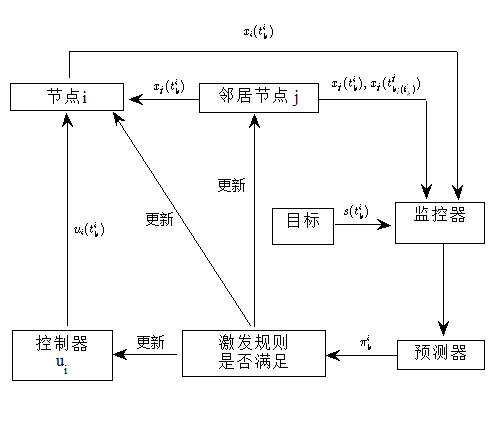
\includegraphics[width=4.5in]{nonlinear/flowchartdec2.png}}
        \end{center}
        \caption{离散监控下的预测激发过程图}\label{flowchart}
        \end{comment}

        与连续监控情形一样, 这里也给出两种不同系统误差上界的激发规则. 不同的是, 离散监控情形下给出的是与系统误差和同步误差相关函数.

        情形c: 基于同步误差上界的离散监控激发规则(简称为DRS激发规则):
        \begin{comment}\label{drule:1}
            \nonumber \pi^{i}_{k}=&\max\Big\{t:
            \sum^N_{j=1,j\neq i}(-l_{ij}(r_{t+t^i_k}))\varphi(t,\xi^i_k,\zeta^j_{k_j(t+t^i_k)},x_i(t^i_k),x_j(t^i_k))\\
             &\quad+\tau d_i(r_{t+t^i_k})\varphi(t,\xi^i_k,0,x_i(t^i_k),s(t^i_k))
            \leq\omega \psi(t,\xi^i_k,0,x_i(t^i_k),s(t^i_k))\Big\},\\
           \nonumber t_{k+1}^i&=t_{k}^i+\pi^{i}_{k},
            \end{comment}
        其中, , , , 函数, , 和的具体定义将会在 中给出.

        情形d: 基于指数函数上界的离散监控激发规则(简称为DRE激发规则):
        \begin{comment}\label{drule:2}
             \nonumber \pi^{i}_{k}=&\max\Big\{t:
            \sum^N_{j=1,j\neq i}(-l_{ij}(r_{t+t^i_k}))\mathrm{E}\varphi(t,\xi^i_k,\zeta^j_{k_j(t+t^i_k)},x_i(t^i_k),x_j(t^i_k))\\
            &\quad+\tau d_i(r_{t+t^i_k})\mathrm{E}\varphi(t,\xi^i_k,0,x_i(t^i_k),s(t^i_k))
            \leq ae^{-b(t+t^i_k)}\Big\},\\
            \nonumber t_{k+1}^i&=t_{k}^i+\pi^{i}_{k},
            \end{comment}
        其中和是正数.
        \begin{rem}
            离散监控下的激发规则分为两个部分, 一个是预测部分, 另一个是判断部分. 预测部分是整个激发规则最主要部分. 相比于连续的监控激发规则, 离散监控激发规则具有更大的计算复杂度.
        \end{rem}
            \begin{algo}[离散监控事件激发算法]\label{algo2}~~

             对所有, 初始化: ;

             当时, 控制器收集节点状态信息以及并传递给预测机制;

             预测机制根据 或者 预测下一次事件激发间隔;

             当时, 如果存在某个邻居节点的事件被激发, 则, 返回;

             如果的状态发生转移, 则返回;

             当时, 则节点的事件被激发, 新的事件激发时刻. 此时节点以及它的邻居节点和控制器将会更新, 即利用时的状态信息替换时的状态信息, 返回.
             \end{algo}

        在给出本节定理前, 先证明如下引理:
         \begin{lem}\label{lem:7}
            若函数满足条件, 即存在常数, 使得对任意有成立, 则函数 满足QUAD条件.
        \end{lem}
        \begin{proof}
            取, 则根据 和Lipschitz条件可得
            \begin{comment}
              &\quad(x-y)^\top G[f(x)-f(y)-\Delta(x-y)]\\
              &=(x-y)\top[f(x)-f(y)]-(1+\frac{l^2}{2})(x-y)^\top(x-y)\\
              &\leq\frac{1}{2}(x-y)^\top(x-y)+\frac{1}{2}(f(x)-f(y))^\top(f(x)-f(y))-(1+\frac{l^2}{2})(x-y)^\top(x-y)\\
              &\leq-\frac{1}{2}(1+l^2)(x-y)^\top(x-y)+\frac{l^2}{2}\| x-y\|^2\\
              &=-\frac{1}{2}(x-y)^\top G(x-y).
            \end{comment}
            因此根据, 函数满足QUAD条件.
        \end{proof}

        \begin{thm}\label{thm:qn}
            如果假设  成立, 以及, 并且存在正定对角阵, , 使得对任意, 有
            \begin{comment}
            \bar{\delta}P(u)\otimes G-c\theta\underline{\alpha} P(u)L(u)\otimes G\Gamma
            -c\tau\underline{\alpha} P(u)D(u)\otimes G\Gamma+\frac{1}{2}\sum_{v=1}^{m}q_{uv}P(v)\otimes G\leq 0,
            \end{comment}
            其中, ,
            那么, 基于激发规则或者激发规则, 按照算法 , 网络系统  可以实现均方指数同步.
        \end{thm}
        \begin{proof}
        该定理的条件与 的条件是一样的, 唯一不同的是事件激发规则. 因此主要证明思路是考察在离散监控事件激发规则成立的条件下连续监控事件激发规则是否也成立. 这只要判断的上界函数和的下界函数是否是和即可. 当时, 首先估计的上界函数. 显然满足如下方程:
            \begin{comment}\label{sys:discrete}
                \bigg\{\begin{array}{c}
                    \dot{x}_i(t)=f(x_i(t))+z_i(r_t,t^i_k), \quad    \\
                    \dot{x}_j(t)=f(x_j(t))+z_j(r_t,t^j_{k_j(t)}),
                \end{array}\\
            \end{comment}
       这里,
       和的定义如下:
        \begin{comment}\label{zi}
        \nonumber z_\iota(r_t,t^\iota_k)&=-\theta(t)\rho(t)\sum^N_{j=1}l_{\iota j}(r_{t})\Gamma[h(x_{j}(t_{k}^{\iota}))-h(x_{\iota }(t_{k}^{\iota}))]\\
        &\quad-\tau\rho(t)d_{\iota}(r_{t})\Gamma[h(x_{\iota}(t_{k}^{\iota}))-h(s(t_{k}^{\iota}))].
        \end{comment}
        为了讨论的方便, 将方程组  抽象为一般形式:
            \begin{comment}\label{sys:dis-gener}
                \bigg\{\begin{array}{c}
                    \dot{u}=f(u)+\xi,   \\
                    \dot{v}=f(v)+\zeta,
                \end{array}
            \end{comment}
       其中.
        根据 可得
            \begin{comment}\label{equ:12}
            \nonumber&\quad\|(h(u)-h(u_0))-(h(v)-h(v_0))\|^2\\
            \nonumber &=\sum^n_{k=1}[ (h_k(u^k)-h_k(u^k_0))-(h_k(v^k)-h_k(v^k_0))]^2\\
            \nonumber &=\sum^n_{k=1}[(h_k(u^k)-h_k(u^k_0))^2+(h_k(v^k)-h_k(v^k_0))^2]\\
            \nonumber &\quad-2\sum^n_{k=1}(h_k(u^k)-h_k(u^k_0))(h_k(v^k)-h_k(v^k_0)) \\
            \nonumber &\leq \bar{\beta}^2\sum^n_{k=1}[ (u^k-u^k_0)^2+(v^k-v^k_0)^2]
            -2\sum^n_{k=1}(h_k(u^k)-h_k(u^k_0))(h_k(v^k)-h_k(v^k_0))\\
            \nonumber &=\bar{\beta}^2\sum^n_{k=1}[(u^k-u^k_0)-(v^k-v^k_0)]^2+\varrho\\
            &=\bar{\beta}^2\|(u-u_0)-(v-v_0)\|^2+\varrho,
            \end{comment}
           其中, .
            对进一步线性化可得:
            \begin{comment}\label{equ:13}
            \nonumber \varrho&\leq\sum^n_{k=1}[2\bar{\beta}^2(u^k-u^k_0)(v^k-v^k_0)+(h_k(u^k)-h_k(u^k_0))^2+(h_k(v^k)-h_k(v^k_0))^2]\\
            \nonumber &\leq\sum^n_{k=1}[2\bar{\beta}^2(u^k-u^k_0)(v^k-v^k_0)+\bar{\beta}^2(u^k-u^k_0)^2+\bar{\beta}^2(v^k-v^k_0)^2]\\
            \nonumber &=\bar{\beta}^2\sum^n_{k=1}(u^k-u^k_0+v^k-v^k_0)^2\\
            &=\bar{\beta}^2\| u-u_0+v-v_0 \|^2.
            \end{comment}
        将式 代入式 可得
            \begin{comment}\label{equ:up1}
            \nonumber &\quad\|(h(u)-h(u_0))-(h(v)-h(v_0))\|^2\\
            &\leq\bar{\beta}^2\|(u-u_0)-(v-v_0)\|^2+\bar{\beta}^2\| u-u_0+v-v_0 \|^2.
            \end{comment}
        因为属于函数类, 根据方程 , 有
            \begin{comment}\label{equ:up2}
            \nonumber &\quad\|(u(t)-u_0)-(v(t)-v_0)\|\\
            \nonumber &=\|\int^t_0[f(u(s))-f(v(s))]ds+(\xi-\zeta)t\|\\
            \nonumber &\leq\int^t_0\|f(u(s))-f(v(s))\|ds+\|\xi-\zeta\|t\\
            \nonumber &\leq l_1\int^t_0\|u(s)-v(s)\|ds+|\xi-\zeta\|t\\
             &\leq l_1\int^t_0\|(u(s)-u_0)-(v(s)-v_0)\|ds+(\|\xi-\zeta\|+l_1\|u_0-v_0\|)t.
            \end{comment}
        类似地
            \begin{comment}\label{equ:up3}
            \nonumber &\quad\| (u(t)-u_0)+(v(t)-v_0)\|\\
            \nonumber &=\|\int^t_0t[f(u(s))+f(v(s))]ds+(\xi+\zeta)t\|\\
            \nonumber &\leq\int^t_0\|f(u(s))+f(v(s))\|ds+\|\xi+\zeta\|t\\
            \nonumber &\leq l_2\int^t_0\|u(s)+v(s)\|ds+\|\xi+\zeta\|t\\
             &\leq l_2\int^t_0\|(u(s)-u_0)+(v(s)-v_0)\|ds+(\|\xi+\zeta\|+l_2\|u_0+v_0\|)t.
            \end{comment}
        对式  和式  分别应用GronwallBellman不等式, 可得
            \begin{comment}\label{equ:up4}
            \|(u(t)-u_0)-(v(t)-v_0)\|\leq\eta_1(\exp^{l_1t}-1),
            \end{comment}
       其中;
            \begin{comment}\label{equ:up5}
            \|(u(t)-u_0)+(v(t)-v_0)\|\leq\eta_2(\exp^{l_2t}-1),
            \end{comment}
       其中.\\
       结合式 、 和  可得
            \begin{comment}\label{equ:up6}
            \|(h(u)-h(u_0))-(h(v)-h(v_0))\|\leq\varphi(t,\xi,\zeta,u_0,v_0),
            \end{comment}
        其中.
        因此的上界函数已得到.

        接下来估计的下界函数. 根据 和方程  可得
            \begin{comment}\label{equ:low1}
            \nonumber &\quad\frac{d}{dt}[(u(t)-v(t))^\top(u(t)-v(t))]\\
            \nonumber &=2(u(t)-v(t))^\top(f(u(t))-f(v(t))+\xi-\zeta)\\
            \nonumber &=2(u(t)-v(t))^\top(f(u(t))-f(v(t)))+2(u(t)-v(t))^\top(\xi-\zeta)\\
            \nonumber &\geq 2\sigma(u(t)-v(t))^\top(u(t)-v(t))+2(u(t)-v(t))^\top(\xi-\zeta)\\
            \nonumber &\geq 2\sigma(u(t)-v(t))^\top(u(t)-v(t))-\sigma(u(t)-v(t))^\top(u(t)-v(t))-\frac{1}{\sigma}(\xi-\zeta)^\top(\xi-\zeta)\\
            &=\sigma(u(t)-v(t))^\top(u(t)-v(t))-\frac{1}{\sigma}(\xi-\zeta)^\top(\xi-\zeta).
            \end{comment}
        通过利用, 可以推出
        \begin{comment}\label{equ:low3}
        (u(t)-v(t))^\top(u(t)-v(t))\geq (u_0-v_0)^\top(u_0-v_0)e^{\sigma t}-\frac{(\xi-\zeta)^\top(\xi-\zeta)}{\sigma^2}(e^{\sigma t}-1).
        \end{comment}
        由于对任意,式  右端在小区间上是正数, 故有
        \begin{comment}\label{equ:low4}
        \| u(t)-v(t)\|\geq \psi(t,\xi,\zeta,u_0,v_0),
        \end{comment}
        其中


        综上所述, 如果激发规则DRS满足, 那么根据式  和 , 激发规则CRS也满足. 类似地, 如果激发规则DRE满足, 那么根据式 , 激发规则CRE 也满足. 因此根据 的结论, 网络系统  可以实现均方指数同步.
        \end{proof}
        \begin{rem}
        几何上, 可以看作是在映射下和从时刻 到时刻的位移差的上界函数, 而可以看作是和在时刻的距离的下界函数.
        \end{rem}
        \begin{rem}
        在DRS激发规则中, 从时刻到时刻轨道之间的位移差的上界函数被同步误差的下界函数控制, 而在DRE激发规则中, 从时刻到时刻轨道之间的位移差的上界函数被可由参数, 调节收敛速度的指数函数控制. 因此DRS激发规则的同步速度比DRE激发规则快, 但DRS激发规则的激发次数比DRE激发规则高. 故在选择激发规则时, 需要在收敛速度和激发次数之间进行取舍. 如果状态监控、数据更新、信号通讯成本较低, 对同步速度要求不高的情况下, 则选用DRE激发规则并选择较大的参数, , 否则选择DRS 激发规则较好.
        四种激发函数的各方面特征比较如下:
        \end{rem}
\begin{table}[!hbp]
\setlength{\abovecaptionskip}{-1pt}
\setlength{\belowcaptionskip}{-1pt}
\caption{四种激发规则的特征比较}\label{table11}
\begin{center}
\begin{tabular}{|c|c|}
\hline
~~~同步速度~~~ & ~~~CRSDRS, CREDRE~~~\\
\hline
~~~监控成本~~~ & ~~~CRSCREDRSDRE~~~\\
\hline
~~~计算负荷~~~ & ~~~DRSDRECRSCRE~~~\\
\hline
~~~激发次数~~~ & ~~~DRSDRECRSCRE~~~\\
\hline
\end{tabular}
\end{center}
\end{table}
        \begin{rem}
        连续监控激发规则和离散监控激发规则最大的区别在于收集节点状态信息时刻的不同, 在连续监控情形中, 监控器需要不停地监控网络所有节点状态并收集记录其状态信息, 激发规则需要根据收集到数据进行实时更新, 即激发规则每时每刻都需要计算和判断条件是否满足. 而在离散监控激发规则中, 监控器只在事件激发时刻监控节点状态, 当某个节点的事件激发时, 监控器把该节点状态信息传递给预测机制, 预测机制根据收集得到的信息进行预测下一次激发时刻, 即激发规则是需要在激发时刻对数据进行更新.
        \end{rem}
\section{数值模拟}
        本节给出一个数值例子去验证前文提出定理结论的有效性, 并在数值例子中比较四种激发规则的性能. 该例子考虑含有个节点的复杂网络, 每个节点都有个不同的状态组成. 网络模型如下:
        \begin{comment}\label{simulate}
        \nonumber\dot{x}_{i}(t)=&f(x_{i}(t))-\theta(t)\rho(t)\sum^{100}_{j=1}l_{ij}(r_{t})\Gamma[h(x_{j}(t_{k}^{i}))-h(x_{i}(t_{k}^{i}))]+u_i(t),\\
         &\quad t_{k}^i\leq t< t_{k+1}^i, \quad i = 1,\cdots,100.\\
        \nonumber u_i(t)=&-\tau \rho(t)d_{i}(r_{t})\Gamma[h(x_{i}(t_{k}^{i}))-h(s(t_{k}^{i}))],
        \end{comment}
\begin{comment}[!htb]
\begin{minipage}[t]{0.48\linewidth}
\centering
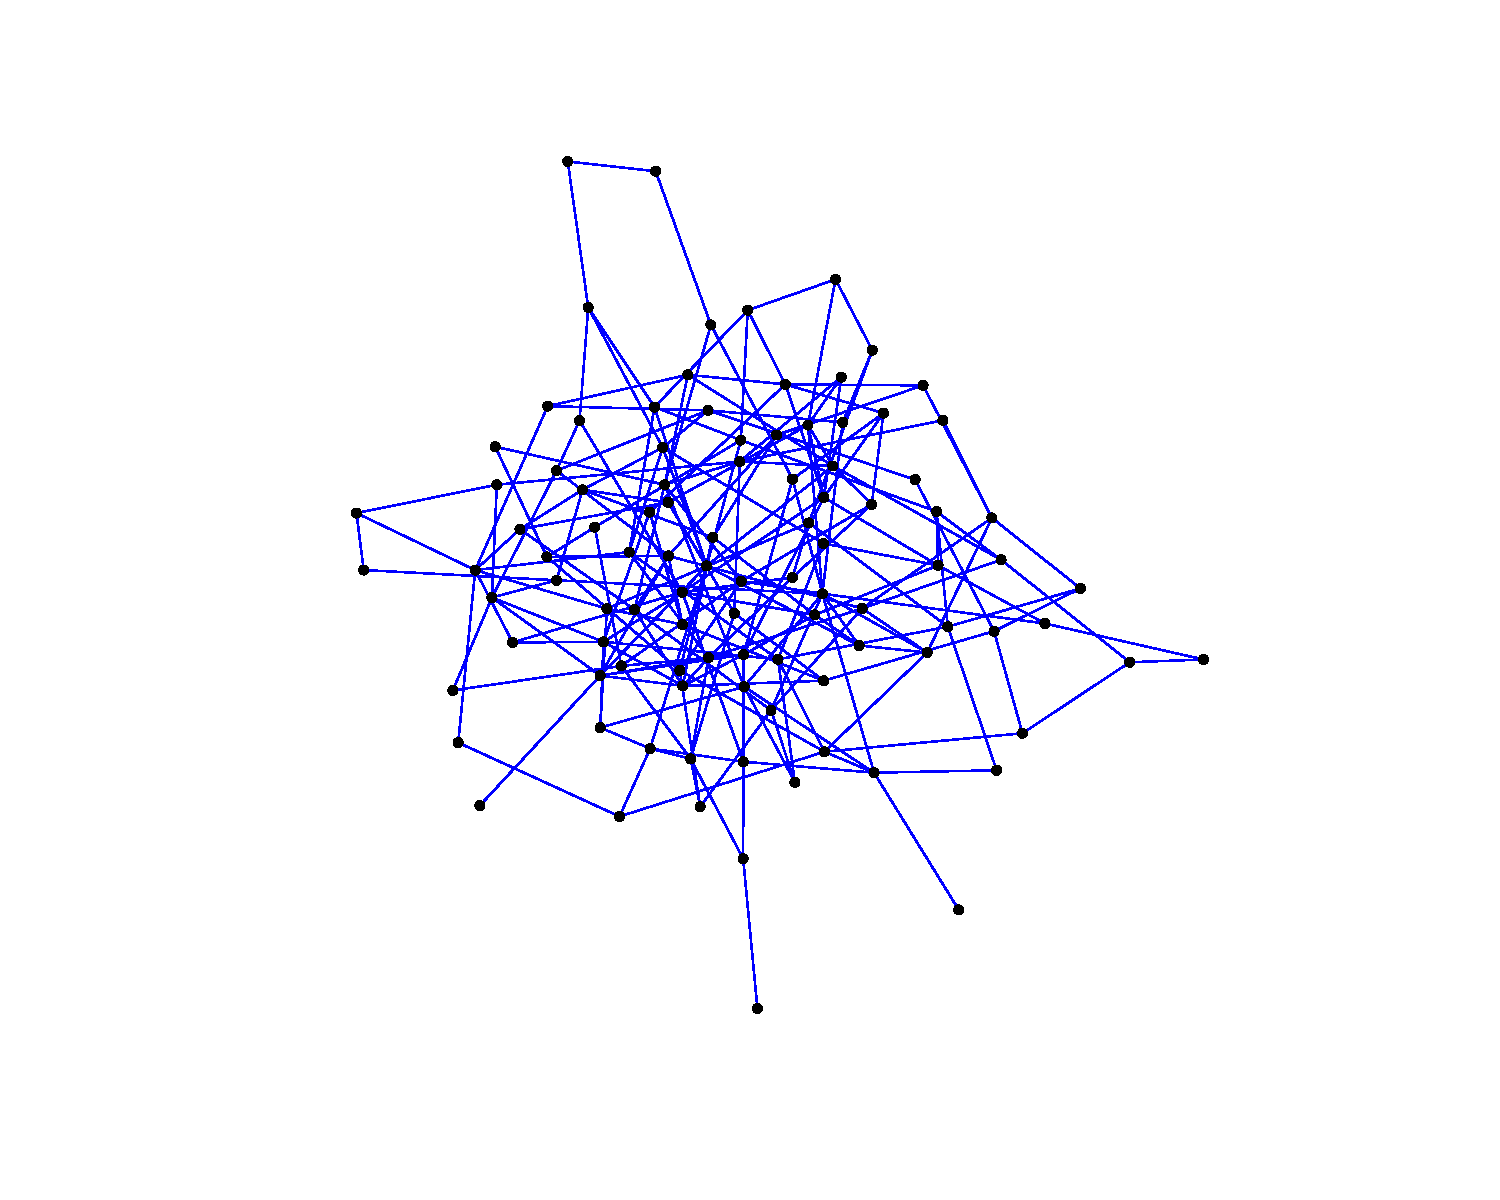
\includegraphics[width=3.2in]{nonlinear/NewL1.pdf}
\caption{马尔可夫链处在状态下的网络拓扑结构.}\label{topology1}
\end{minipage}~~
\begin{minipage}[t]{0.48\linewidth}
\centering
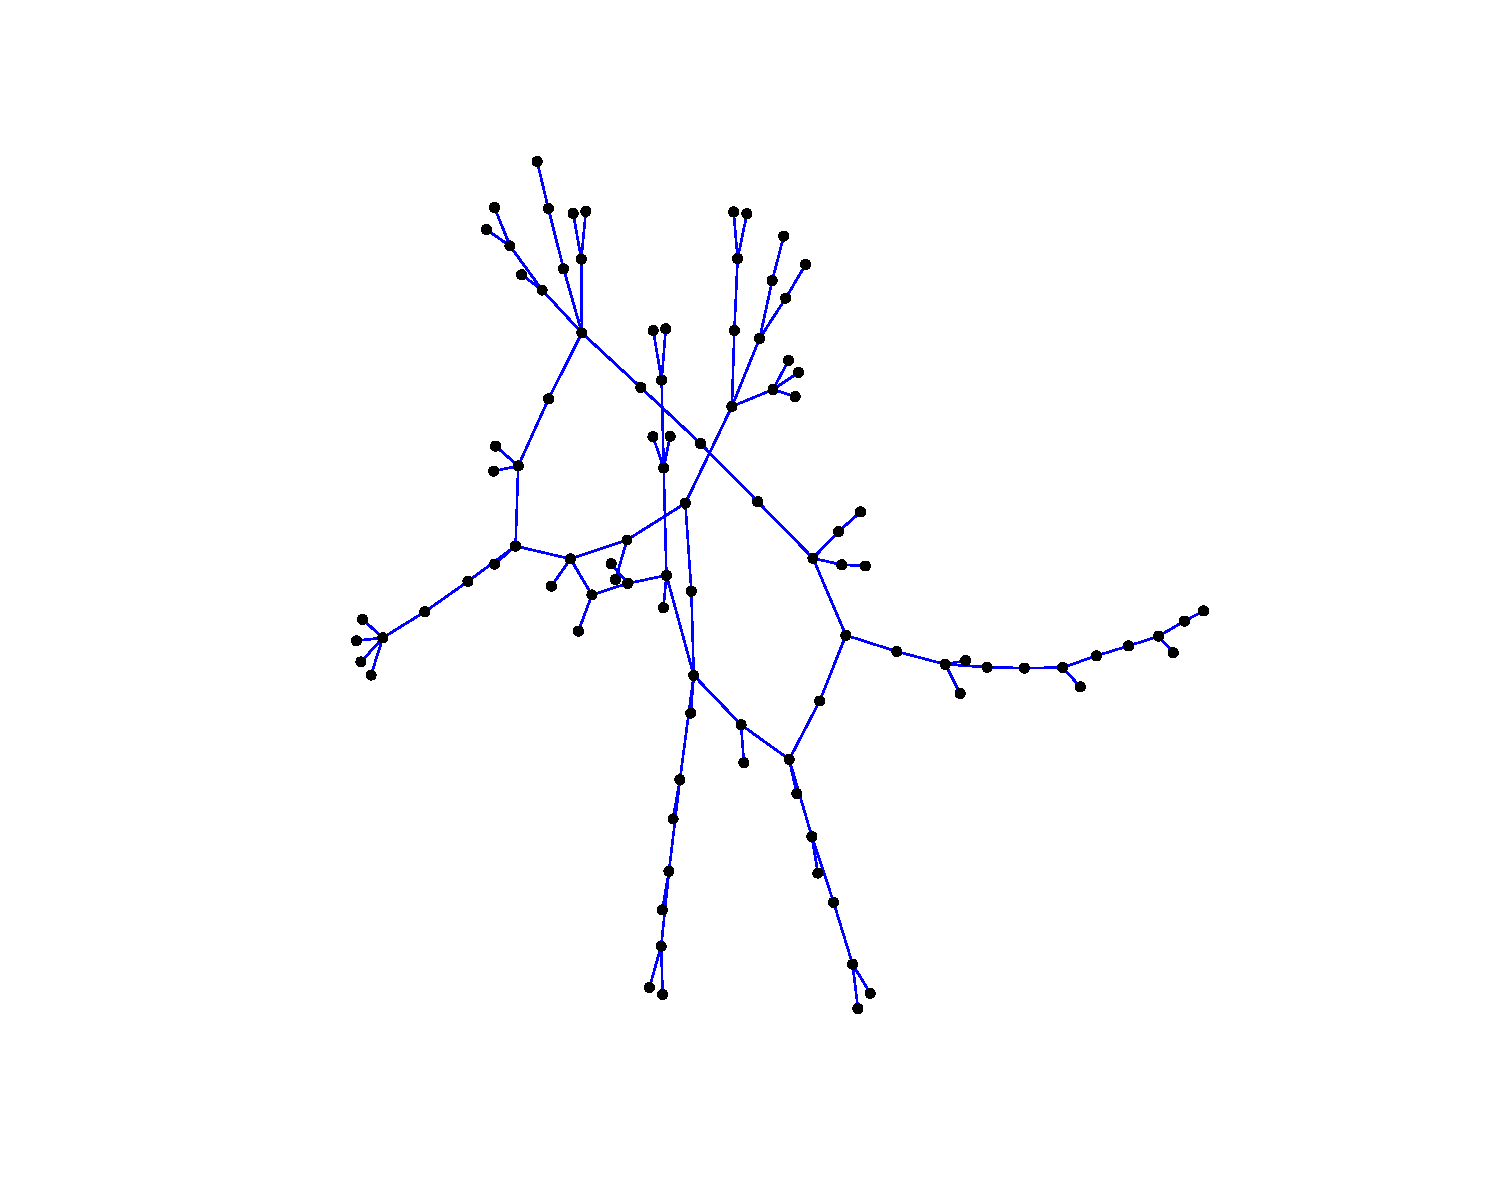
\includegraphics[width=3.2in]{nonlinear/NewL2.pdf}
\caption{马尔可夫链处在状态下的网络拓扑结构.}\label{topology2}
\end{minipage}
\end{comment}
\begin{comment}[!htb]
\begin{minipage}[t]{0.48\linewidth}
\centering
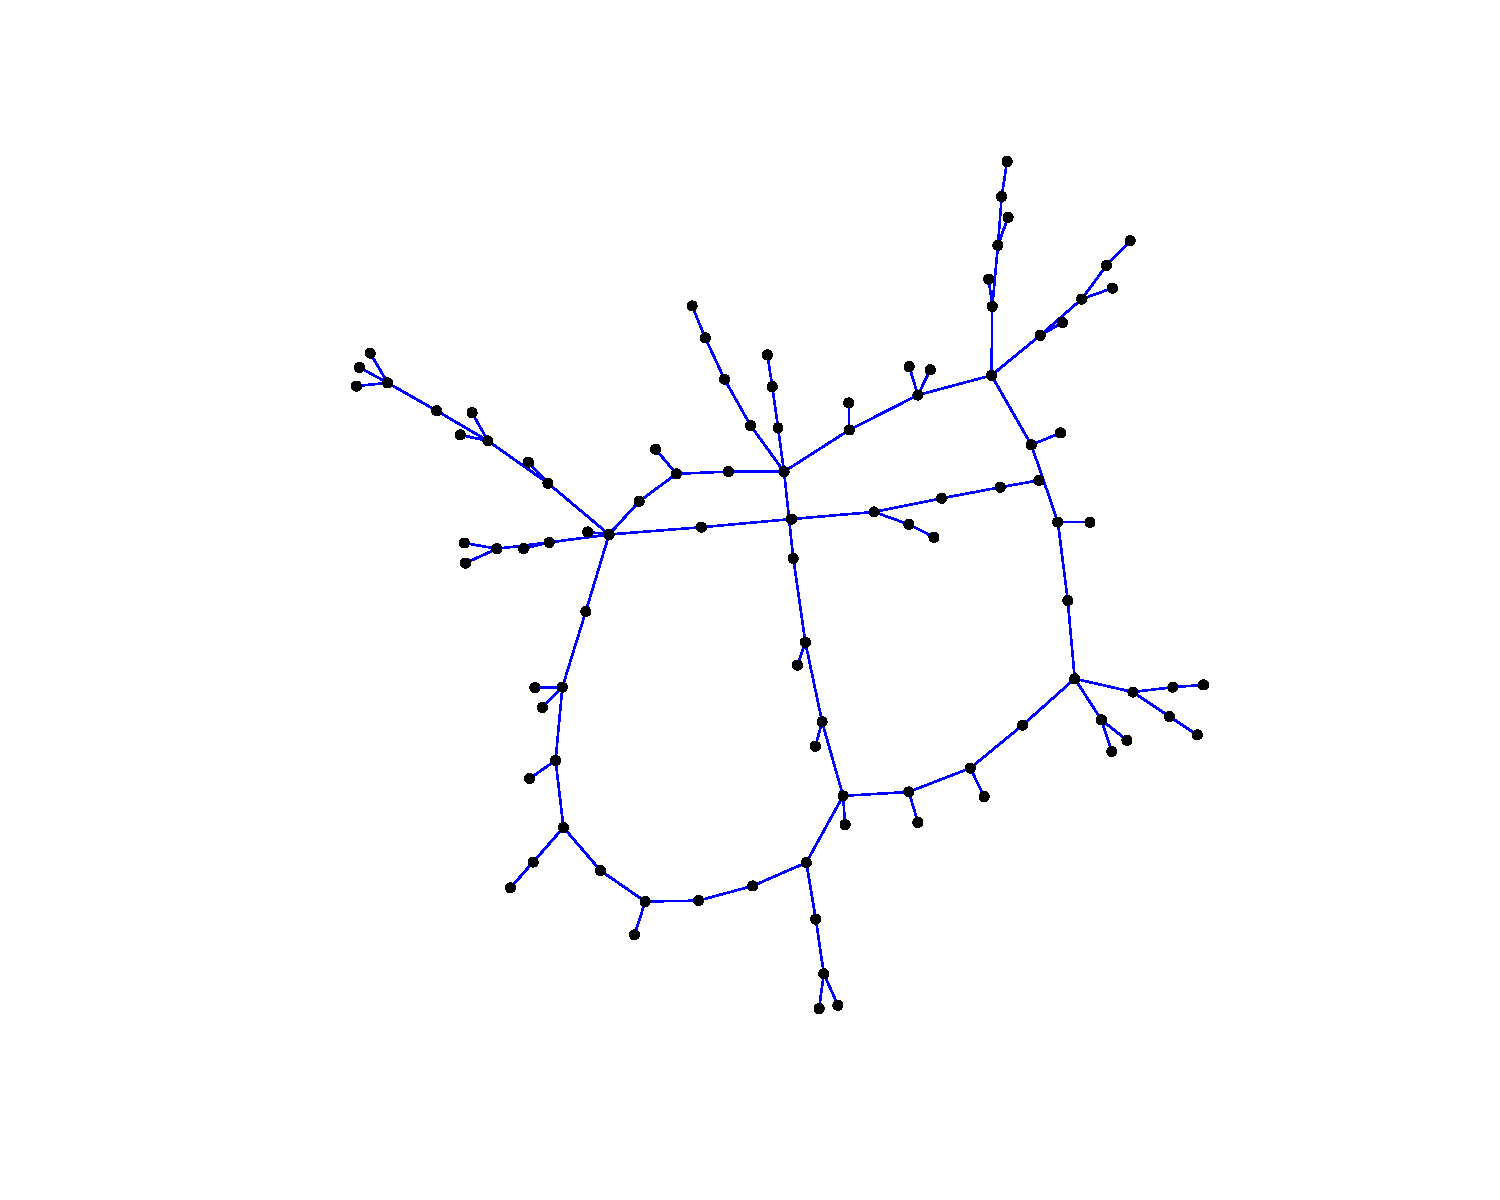
\includegraphics[width=3.2in]{nonlinear/NewL3.pdf}
\caption{马尔可夫链处在状态下的网络拓扑结构.}\label{topology3}
\end{minipage}~~
\begin{minipage}[t]{0.48\linewidth}
\centering
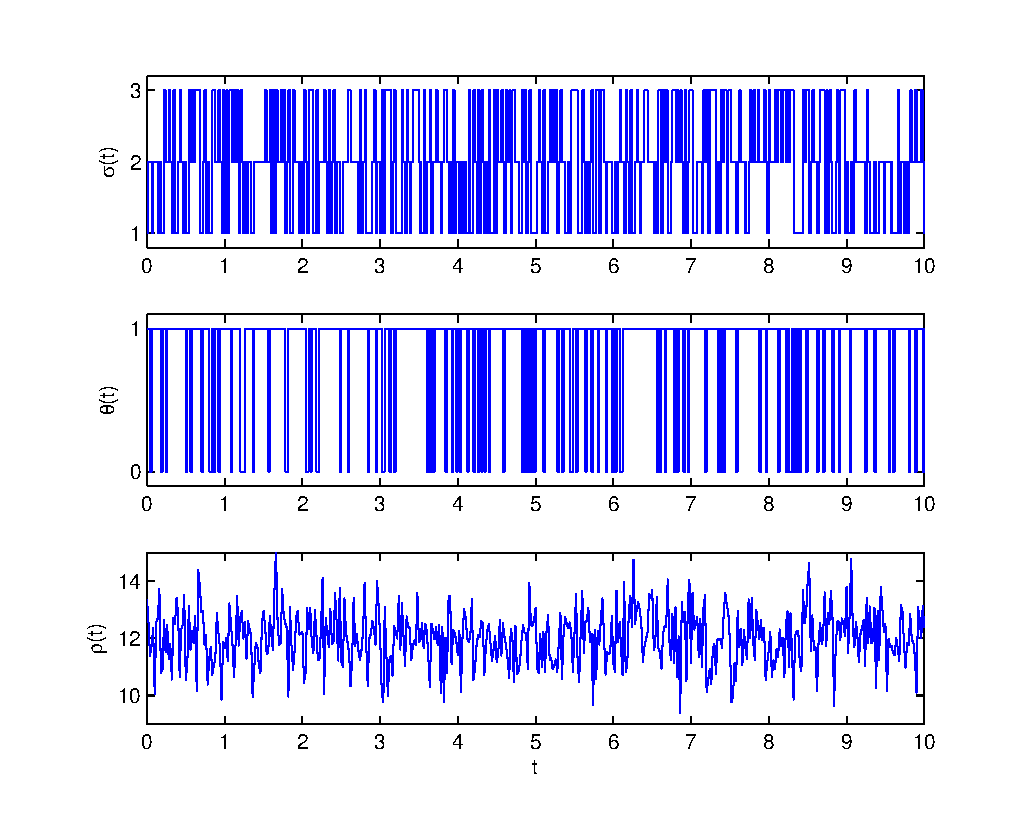
\includegraphics[width=3.2in]{nonlinear/randomvariabel.eps}
\caption{马尔可夫链和随机变量的变化图.}\label{random}
\end{minipage}
\end{comment}
        其中网络可能的拓扑结构见、 和 , 这里选择著名的蔡氏电路系统作为自动力学性态, 它的动力学方程为:
        \begin{comment}
           f(x)=\left(
                  \begin{array}{c}
                    z_1(-x_1+x_2-g(x_1)) \\
                    x_1-x_2+x_3 \\
                    -z_2(x_2) \\
                  \end{array}
                \right)
           \end{comment}
        其中, .
        非线性耦合函数以及状态空间为的马尔可夫链的转移率矩阵如下所示:
           \begin{comment}
           h(x)=\left(
                  \begin{array}{c}
                    2x_1+0.2\sin x_1 \\
                    2x_2+1 \\
                    3x_3+0.5\cos x_3 \\
                  \end{array}
                \right),~~~~
           Q=\left(
            \begin{array}{ccc}
              -8 & 4 & 4 \\
              5 & -8 & 3 \\
              1 & 7 & -8 \\
            \end{array}
          \right).
           \end{comment}
        根据定义, 通过计算可知, 取可是得满足. 可能的牵制控制节点为: , .
        是参数为伯努利随机变量, 是参数为的正态随机变量. 其演变情况如 所示.
\begin{comment}[!htb]
\begin{minipage}[t]{0.48\linewidth}
\centering
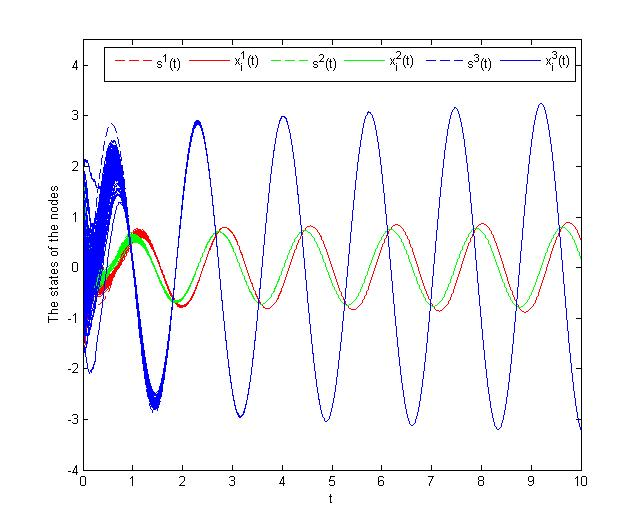
\includegraphics[width=3.2in]{nonlinear/state2223.jpg}
\caption{在连续监控激发规则CRS下, 网络节点状态向量和目标轨道随时间变化情况.}\label{numcrule1}
\end{minipage}~~
\begin{minipage}[t]{0.48\linewidth}
\centering
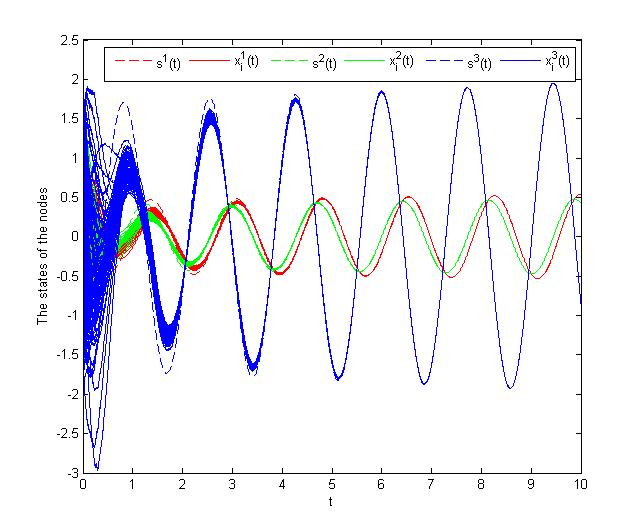
\includegraphics[width=3.2in]{nonlinear/state1612.jpg}
\caption{在连续监控激发规则CRE下, 网络节点状态向量和目标轨道随时间变化情况.}\label{numcrule2}
\end{minipage}
\end{comment}

\begin{comment}[!htb]
\begin{minipage}[t]{0.48\linewidth}
\centering
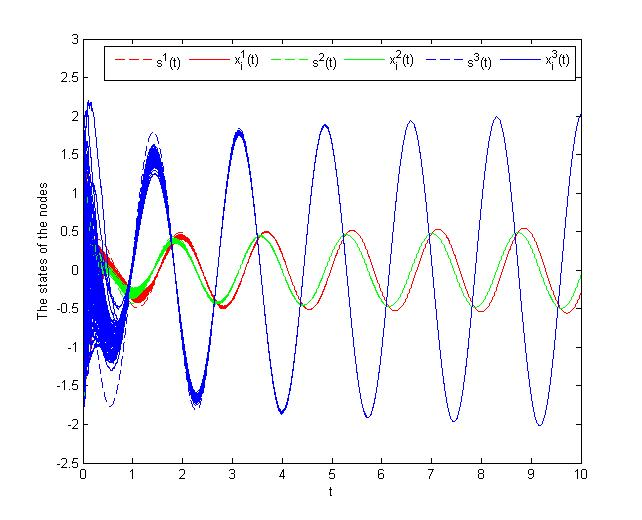
\includegraphics[width=3.2in]{nonlinear/dstateoneand2212.jpg}
\caption{在离散监控激发规则DRS下, 网络节点状态向量和目标轨道随时间变化情况.}\label{numdrule1}
\end{minipage}~~
\begin{minipage}[t]{0.48\linewidth}
\centering
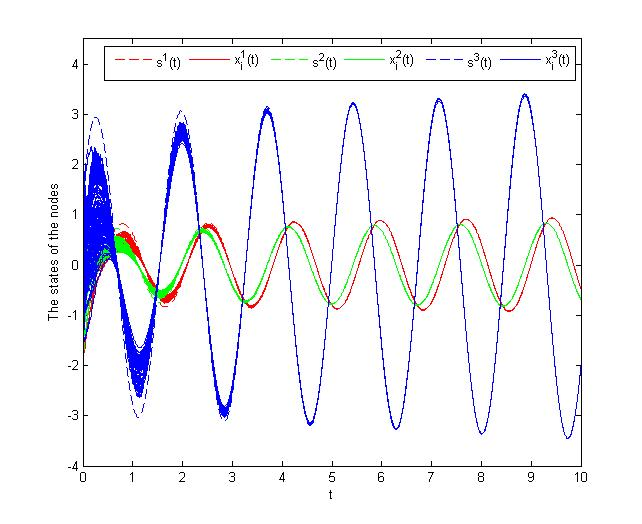
\includegraphics[width=3.2in]{nonlinear/dstatedata3840.jpg}
\caption{在离散监控激发规则DRE下, 网络节点状态向量和目标轨道随时间变化情况.}\label{numdrule2}
\end{minipage}
\end{comment}

        下面选择相应的参数使得 和 的条件成立.
        取, . 通过对函数求偏导数可得其可能的Jacobin矩阵为:
        \begin{comment}
        \left(
              \begin{array}{ccc}
                3.0318 & 9.78 & 0 \\
                1 & -1 & 1 \\
                0 & -14.97 & 0 \\
              \end{array}
            \right),~~~~
        \left(
              \begin{array}{ccc}
                -2.445 & 9.78 & 0 \\
                1 & -1 & 1 \\
                0 & -14.97 & 0 \\
              \end{array}
            \right).
        \end{comment}
        因此取, 其中是Jacobin矩阵对称部分的最大特征值.
\begin{comment}[!htb]
\begin{minipage}[t]{0.48\linewidth}
\centering
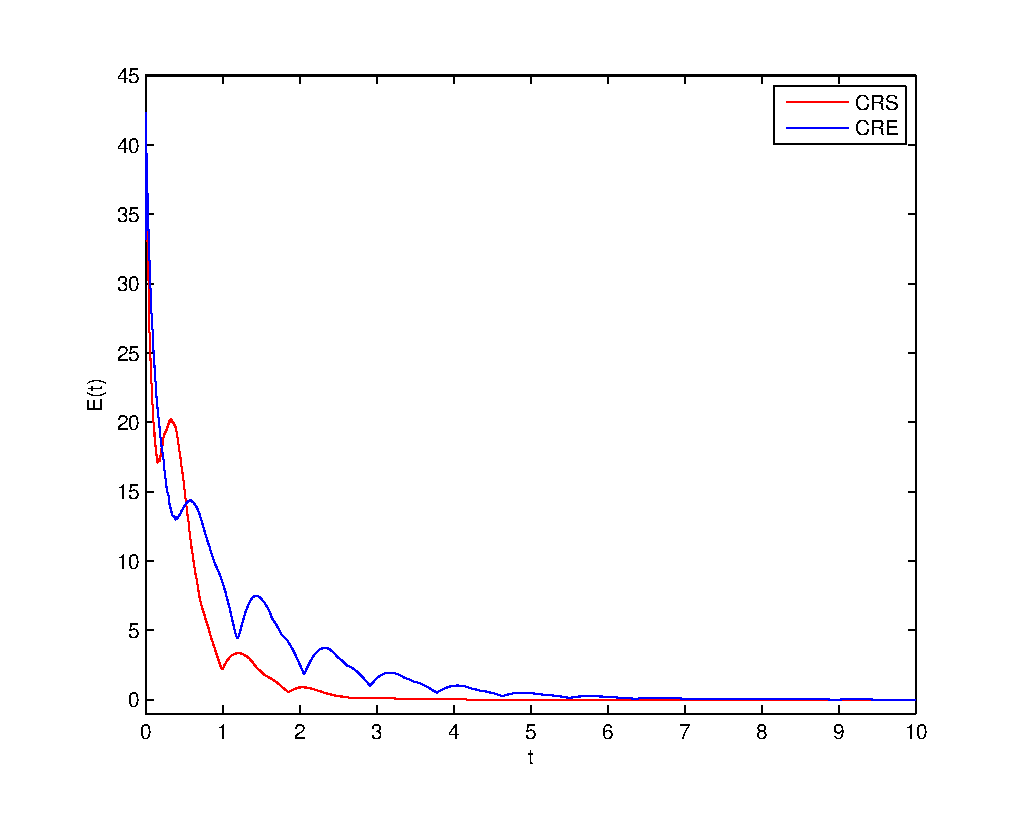
\includegraphics[width=3.2in]{nonlinear/Totallerror1.eps}
\caption{在连续监控激发规则CRS和激发规则CRE下, 网络总误差轨道随时间变化情况.}\label{Totallerror1}
\end{minipage}~~
\begin{minipage}[t]{0.48\linewidth}
\centering
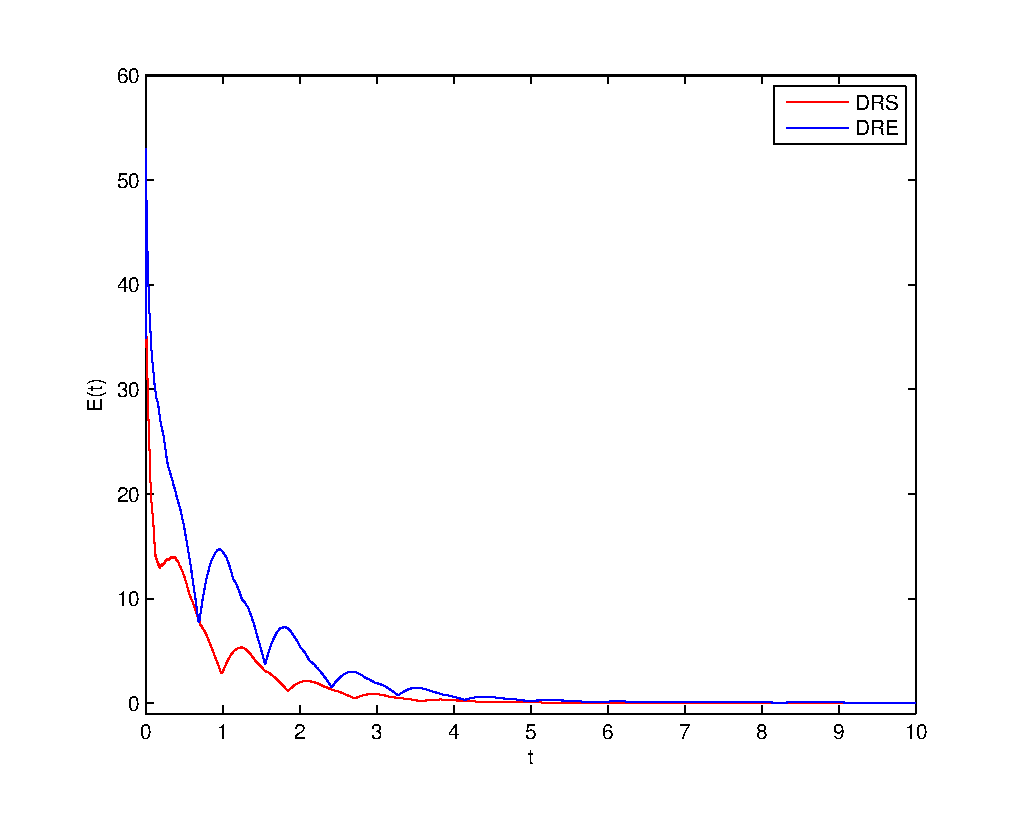
\includegraphics[width=3.2in]{nonlinear/Totallerror2.eps}
\caption{在离散监控激发规则DRS和激发规则DRE下, 网络总误差轨道随时间变化情况.}\label{Totallerror2}
\end{minipage}
\end{comment}
\begin{comment}[!htb]
\begin{minipage}[t]{0.48\linewidth}
\centering
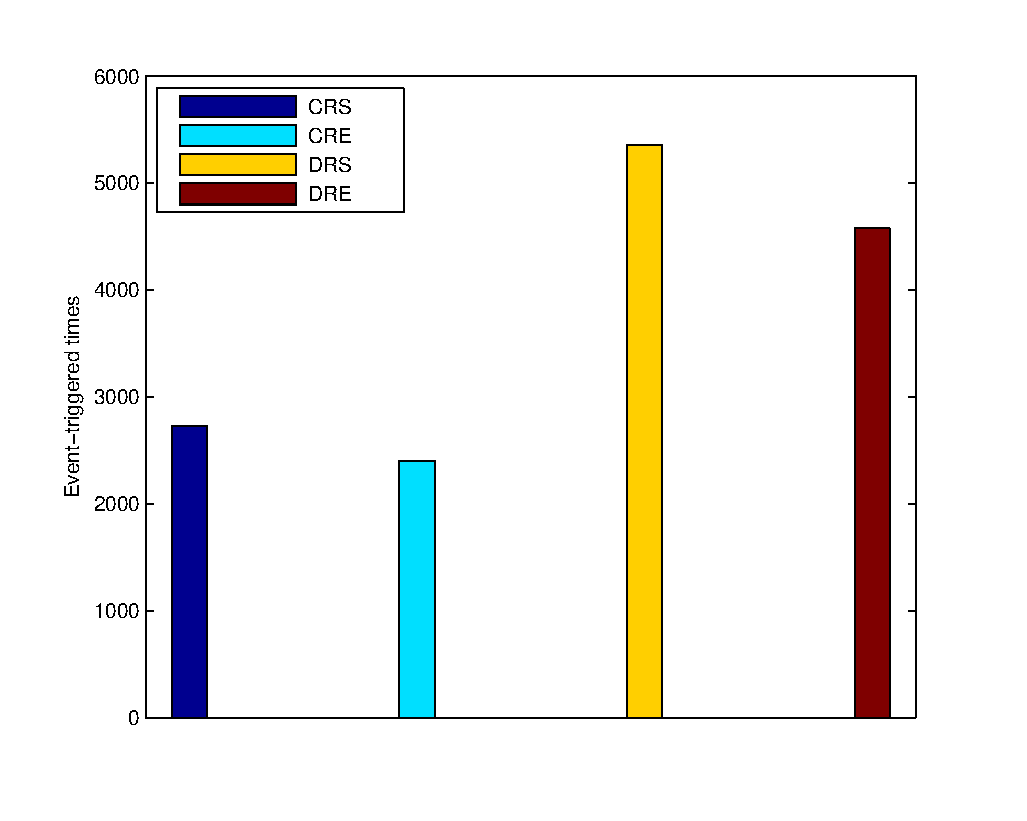
\includegraphics[width=3.2in]{nonlinear/triggertime.eps}
\caption{连续监控和离散监控四种激发规则每个节点平均激发次数.}\label{tritime}
\end{minipage}~~
\begin{minipage}[t]{0.48\linewidth}
\centering
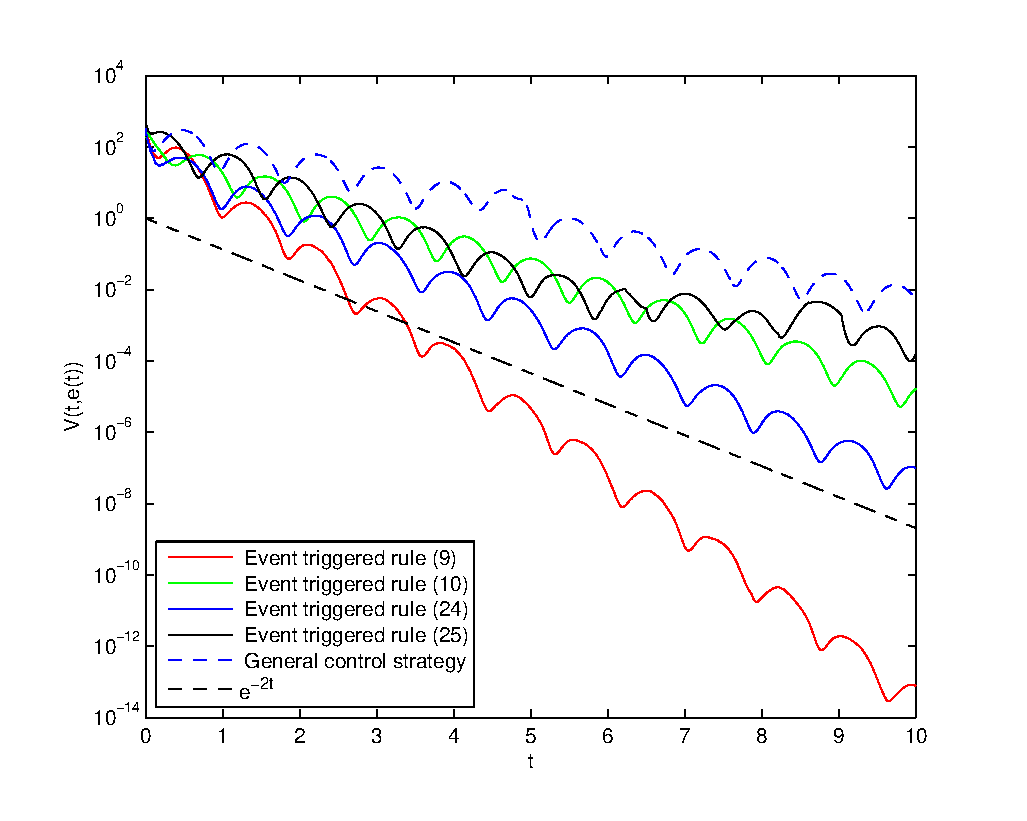
\includegraphics[width=3.2in]{nonlinear/Vt.eps}
\caption{Lyapunov-Krasovskii函数.}\label{Vt}
\end{minipage}
\end{comment}
        接下来估计参数, 根据微分中值定理可得:
        \begin{comment}
        \quad(f(u)f(v))^\top((f(u)-f(v)))
        &=(J(\varsigma)(u-v))^\top(J(\varsigma)(u-v))\\
        &=(u-v)^\top J(\varsigma)^\top J(\varsigma)(u-v)\\
        &\leq\lambda_{max}(J(\varsigma)^\top J(\varsigma))(u-v)^\top(u-v)\\
        &\leq17.9826^2(u-v)^\top(u-v)
        \end{comment}
        故取可使得. 记或者, , 于是
        \begin{comment}
         &\quad\| f(x)+f(s)\|^2\\
         &=(-\nu\mu_1+z_1)^2+(\mu_1-\mu_2+\mu_3)^2+(z_2\mu_2)^2\\
         &=(\nu^2+1)\mu_1^2+(z_1^2+z_2^2+1)\mu_2^2+\mu_3^2-2(z_1\nu+1)\mu_1\mu_2+2\mu_1\mu_3-2\mu_2\mu_3\\
         &\leq(\nu^2+z_1\nu+3)\mu_1^2+(z_1^2+z_2^2+z_1\nu+3)\mu_2^2+3\mu_3^2\\
         &\leq32.8901\mu_1^2+346.6614\mu_2^2+3\mu_3^2\\
         &\leq18.6188^2\| x+s\|^2.
        \end{comment}
\begin{comment}[!htb]
\begin{minipage}[t]{0.48\linewidth}
\centering
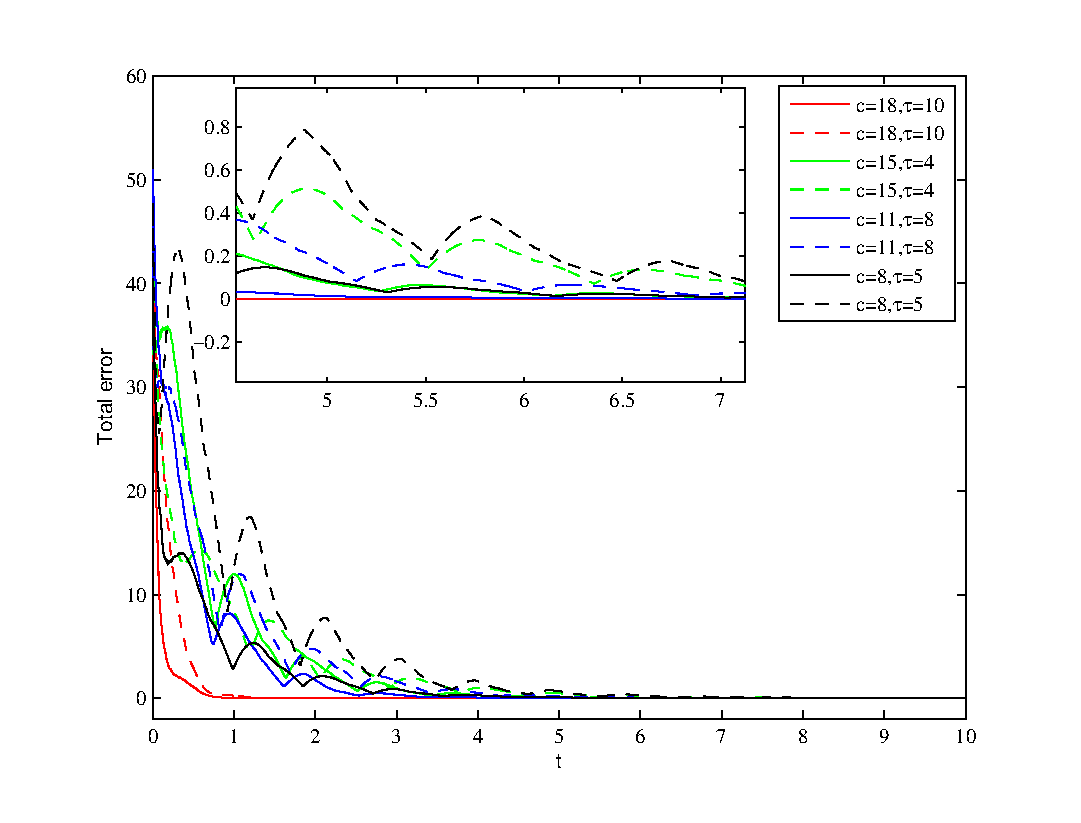
\includegraphics[width=3.2in]{nonlinear/diffstrength.eps}
\caption{连续监控下不同耦合强度和控制强度的系统总误差图, 其中实线表示CRS激发规则, 虚线表示CRE激发规则.}\label{cdiffstrength}
\end{minipage}~~
\begin{minipage}[t]{0.48\linewidth}
\centering
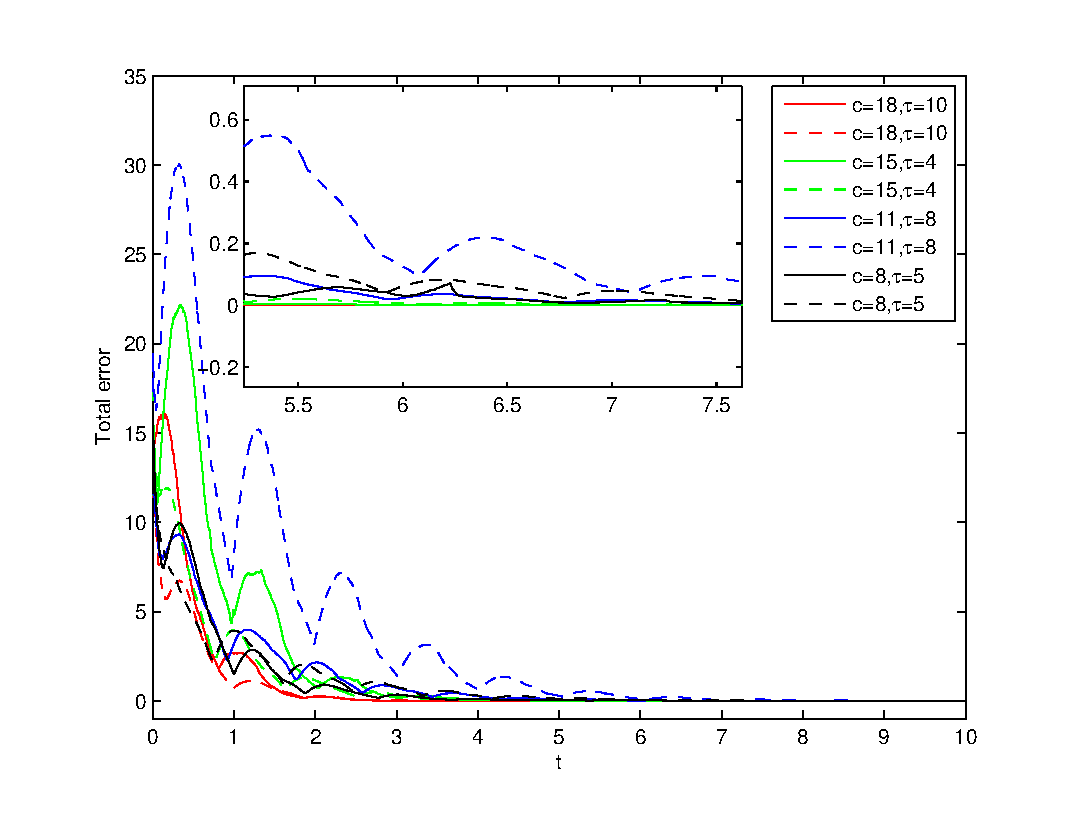
\includegraphics[width=3.2in]{nonlinear/differentstength.eps}
\caption{离散监控下不同耦合强度和控制强度的系统总误差图, 其中实线表示DRS激发规则, 虚线表示DRE激发规则.}\label{ddiffstrength}
\end{minipage}
\end{comment}
       因此取, 可使得. 综上所述, 属于函数类.

        选取, 那么对所有, . 即 和 的条件成立. 取, , 通过计算可得.

        利用欧拉法, 取步长为, 区间为. 通过MATLAB求解微分方程  并画出相应的变化图, 见 至.

         至 展示了在四种激发规则下, 节点状态向量轨道的变化情况. 从图中可以看出, 所有节点的状态都趋于同步. 因此本文提出的激发规则是有效的.

        为了更好的比较四种激发规则的性能, 下面画出不同激发规则下的网络系统总同步误差, 其定义为如下:


         和 描述了在四种激发规则下网络系统总误差随时间变化过程, 从这两个图可以看出, 系统误差都能够趋于零. 但各种激发规则趋于零的时间有稍微的差别. CRS激发规则达到同步所需要的时间比CRE要快一些. DRS激发规则达到同步所需要的时间比DRE要快一些. 即基于误差上界的激发规则有较短的同步时间. 这与 分析的结果一致.


         和  分别是四种激发规则的平均激发次数和Lyapunov—Krasovskii函数. 从图中看出, 离散监控的激发规则的平均激发次数要高于连续情形, 四种激发函数平均激发次序从高到低依次是: DRSDRECRSCRE, 即要使得同步时间较快则需要付出更高的激发次数. 四种激发规则的 收敛速度都比快, 即指数同步已实现. 和 是选择不同耦合强度和控制强度时的系统误差图, 图中可以看出, 耦合强度和控制强度越大, 系统获得同步的时间就越短.

\section{小结}
    在这一章节, 主要研究了一类带有马氏切换非线性耦合的时滞网络, 主要引进了事件激发的牵制控制策略. 分析了连续和离散两种情形下的基于不同误差上界的激发规则, 利用Lyapunov—Krasovskii稳定性理论和Kronecker积的性质推导了充分的均方指数同步条件, 并在数值模拟中比较了四种不同激发规则之间的同步性能以及消耗的成本.
%%!Mode:: "Tex:UTF-8"


\chapter{集中式事件激发采样下带部分未知转移率和时滞的复杂网络同步问题}
    上一章节讨论了基于分散式事件激发采样控制策略下的转移概率已知的马氏切换的复杂网络. 尽管网络模型考虑的切换拓扑的情形, 但是马氏链的转移率是已知的. 特别是多切换拓扑的模型中, 很难去精确获得每个切换拓扑间的转移率. 本章节将切换拓扑的转移率推广到部分未知的情形. 另一方面, 在现实的网络中, 由于信号传输和信息过程的有限速度以及有限带宽, 所以时滞是不可避免的, 如无线通信网络中由于环境噪声等影响用户间的通信会出现同时或滞后的情况. 时滞可能会降低网络的性能和稳定性. 在采样策略上, 本章采用集中式事件激发采样方法, 集中式事件激发采样只有一个激发规则, 所有节点都按照此规则更新. 其特点是花费较少的计算负荷. 但采样频率会较频繁.

    %因此迟滞复杂网络的同步问题已经越来越引起了许多学者们的注意, 并且已成为一个热点话题. 例如, Wang\upcite{M24}利用牵制控制方法研究了带有马氏切换的随机复杂网络同步问题; 随后Zhou\upcite{M23}在Wang的基础上通过脉冲控制和牵制控制方法相结合, 给出了带马氏切换随机网络的簇同步判据; Yang\upcite{randomcoupling1} 研究了非恒同节点时滞和随机耦合强度马氏切换复杂网络的同步问题. 尽管目前关于时滞已经积累了较多成果, 但是大部分的工作都只是没有考虑到随机环境的影响, 特别是切换拓扑, 即使有作者研究考虑了马氏切换情形, 但也是停留在马氏链转移概率全部已知的情况. 目前针对马氏链转移率部分未知的切换拓扑还没有相关成果, 跟不用说利用比较经济的事件激发策略去研究该类网络的同步问题. 除此之外, 同步目标有些情况下是通过节点之间相互协商才得出来的结果, 因此考虑动态的同步目标更具有使用价值.

\section{集中式事件激发采样的网络模型}

        在这一章节, 考虑一个部分未知转移率的马尔可夫链切换拓扑以及自身动力学时滞复杂网络, 在集中式事件激发采样控制策略下的数学模型如下:
        \begin{comment}\label{sys:cen}
           \nonumber \dot{x}_{i}(t)&=f(t,x_{i}(t),x_i(t-\tau))-c\sum^N_{j=1}l_{ij}(r_{t})\Gamma[x_{j}(t_k)-x_{i}(t_{k})]+u_i(t),\\
            &\quad\quad t_{k}\leq t< t_{k+1}, \quad i = 1,\cdots,N,
        \end{comment}
        这里的节点自身动力与前两章的模型相比较多了迟滞因子, 即; 是常量耦合强度;
        是严格递增的激发时刻序列;
        是控制输入, 定义如下:
        \begin{comment}\label{control}
            u_i(t)=-\rho c\beta_{i}(t)\frac{1}{N}\sum_{j=1}^N\Gamma[x_{i}(t_{k})-x_j(t_{k})],
        \end{comment}
        这里是控制强度增益; 是伯努利随机变量, 并且满足: , .
        \begin{rem}
            以上复杂网络模型除了马氏链和自身动力学与上一章不同之外, 该模型的并未提前确定网络的同步目标, 而是由网络节点在演变过程中确定的, 即这是一个动态调整的同步目标. 由于本节并未采用孤立节点的动力学行为作为网络同步目标, 而是采用动态协调的同步目标. 因此这里的控制输入的形式与上一章的控制形式有所不同. 每个节点的控制输入都是与该节点与其余节点的差成正比, 即根据节点自身与邻居节点之间的关系调整控制输入.
        \end{rem}

        由于自身动力学行为包含有迟滞因子, 所以QUAD条件在本章不再适用, 下面给出类似Lipschitz条件的假设:
        \begin{hyp}{\rm\upcite{p29}}\label{ass1}
            对于节点自身动力学, 假设存在两个常数和, 使得对任意的, 有
         \begin{comment}
        \|f(t,x(t),x(t-\tau))-f(t,y(t),y(t-\tau))\|
        \leq\alpha_1\|x(t)-y(t)\|+\alpha_2\|x(t-\tau)-y(t-\tau)\|.
        \end{comment}
        \end{hyp}
    对于一些著名混沌吸引子, 例如蔡氏电路等, 他们的动力学均满足上述假设. 在同步的文献中, 类似的假设已经被广泛地采用.

    下面给出本节至关重要的引理:
        \begin{lem}\label{mainlemma}
            如果半正定矩阵满足行和为零且有且仅有一个零特征根, 则对任意, 只要, 则有, 其中是矩阵最小非零特征值.
        \end{lem}
        \begin{proof}
        由于矩阵是半正定矩阵且有且仅有一个零特征根, 所以矩阵的特征根可以排序为: , 同时存在正交矩阵, , , 使得
        , 其中. 又因为, 所以. 注意到, 故 . 对任意向量, , 存在向量 使得. 根据以及, 可以得出 , 故. 因此.
        \end{proof}
        \begin{lem}[Halanay不等式]{\rm\upcite{delay-inq}}\label{Halanay}
            设 是定义在区间上的非负函数, 并且区间上连续.
            如果存在两个正数, 并且满足, 使得

            则,
            其中, 是方程的最小实根.
        \end{lem}
        定义测量误差, 同步误差, 其中为参考节点.
        于是有, 以及
        \begin{comment}\label{reference}
        s(t)-s(t_k)&=\frac{1}{N}(\mathbf{1}^\top_N\otimes I_n)(x(t)-x(t_k))
        =-\frac{1}{N}(\mathbf{1}_N^\top\otimes I_n)\delta(t),
        \end{comment}
        这里, . 根据式  和式 , 可得
        \begin{comment}
        {u}_i(t)&=-\rho c\beta_i(t)\Gamma(x_i(t_k)-s(t_k))\\
        &=-\rho c\beta_i(t)\Gamma({\delta}_i(t)+x_i(t)-{s}(t)+{s}(t)-{s}(t_k))\\
        &=-\rho c\beta_i(t)\Gamma({\delta}_i(t)+e_i(t)-\frac{1}{N}(\mathbf{1}_N^\top\otimes I_n)\delta(t)).
        \end{comment}

        为了方便, 记, . 由于和, 所以, 根据Kronecker积的性质, 式  可以被写成下式:
        \begin{comment}\label{dxt}
        \nonumber \dot{x}(t)&=f(t,x(t),x(t-\tau))-c[L_{r_t}\otimes\Gamma]({\delta}(t)+e(t))\\
       &\quad-\rho c[B_t\otimes\Gamma][{\delta}(t)+e(t)-(U\otimes I_n)\delta(t)],\quad t_k\leq t<t_{k+1},
        \end{comment}
        其中, . 因为 和, 所以网络系统  的误差系统为:
        \begin{comment}\label{cee}
        \nonumber \dot{e}(t)&=\dot{x}(t)-(U\otimes I_n)\dot{x}(t)\\
        \nonumber&=f(t,x(t),x(t-\tau))-[U\otimes I_n]f(t,x(t),x(t-\tau))
        -c[L_{r_t}\otimes\Gamma]({\delta}(t)+e(t))\\
        \nonumber&\quad-\rho c[B_t\otimes\Gamma][{\delta}(t)+e(t)-(U\otimes I_n)\delta(t)]
        +\rho c[UB_t\otimes\Gamma][{\delta}(t)+e(t)-(U\otimes I_n)\delta(t)]\\
        \nonumber&=f(t,x(t),x(t-\tau))-[U\otimes I_n]f(t,x(t),x(t-\tau))
        -c[(L_{r_t}+\rho B_t-\rho UB_t)\otimes \Gamma]e(t)\\
        &\quad-c[(L_{r_t}+\rho B_t-\rho B_tU-\rho UB_t+\rho UB_tU)\otimes \Gamma]{\delta}(t),\quad t_k\leq t<t_{k+1}.
        \end{comment}
\section{基于集中式事件激发采样的复杂网络同步分析}\label{result}
        下面设置集中式的事件激发策略, 结合随机发生控制的方法给出网络系统  的均方指数同步充分条件, 并且给出事件激发间隔的下界, 以确保在事件激发过程中不会发生事件瞬间累积, 即Zeno 现象. 在给出主要结论前, 先给出一些符号的说明: , , , , .
\subsection{网络的同步判据}
        记, , ,  则有. 定义事件激发函数如下:
        \begin{comment}\label{trirule}
            g(t)=\|\hat{{\delta}}(t)\|-\varpi\|\hat{x}(t)\|,
        \end{comment}
        其中是正数. 当事件激发函数达到阈值时, 系统就会被激发, 激发时刻随即被确定, 即:
        \begin{comment}
            t_{k+1}=\max\{t\ge t_k: g(t)\le 0\}.
        \end{comment}
        \begin{thm}\label{them}
        如果假设成立, 并且存在常数, 使得对任意, 有:
            \begin{comment}\label{thm:1}
            \left\{
            \begin{commented}
            &\pi+a+\pi_u-c\gamma(\lambda_2+\rho\beta)\leq0,\\
            &2a\lambda_2^2-\bar{\lambda}\alpha_2>0,\\
            &L^2_v-a_uI_N\leq 0, \quad\quad \text{if} \quad v\neq u, v\in S_2^u, \\
            &L^2_v-a_uI_N\geq 0, \quad\quad \text{if} \quad v= u, v\in S_2^u,
            \end{commented}
            \right.
            \end{comment}
        其中, $\pi_u=\frac{1}{2}\sum_{v\in S_1^u\setminus\{u\}}q_{uv}(\frac{\bar{\lambda}^2_{v}}{\lambda_2^2}-\frac{a_u}{\bar{\lambda}^2})
        +\frac{1}{2}q_{uu}I(u)(1-\frac{a_u}{\lambda_2^2})u\in S_1^uI(u)=1I(u)=0$.
        那么, 在事件激发函数下, 取, 网络系统对任意初值都可以实现均方指数同步.
        \end{thm}

        \begin{proof}
        定义随机Lyapunov-Krasovskii函数如下:
        \begin{comment}
        V(t)=\frac{1}{2}\hat{e}^\top(t)\hat{e}(t).
        \end{comment}
        记, , 则有:
        \begin{comment}\label{ekt}
        \hat{e}^\top(t)\hat{e}(t)=e^\top(t)[L^2_u\otimes I_n]e(t)=\sum_{k=1}^ne^k(t)^\top L^2_ue^k(t).
        \end{comment}
        因为满足, 所以当且仅当.
        因此当且仅当. 故Lyapunov-Krasovskii是合格的.

        根据式  和, 有:
        \begin{comment}
        \hat{e}^\top(t)\hat{e}(t)=\sum_{k=1}^ne^k(t)^\top L^2_ue^k(t)\geq\lambda_2^2\sum_{k=1}^ne^k(t)^\top e^k(t)=\lambda_2^2e^\top(t)e(t).
        \end{comment}
        因此.

        因为和, 因此有:
        \begin{comment}\label{sys:err}
        \nonumber \mathrm{E}\mathcal{L}V(t)&=\mathrm{E}\Big\{\hat{e}^{\top}(t)\dot{\hat{e}}(t)+\frac{1}{2}\sum_{v=1}^{m}q_{uv}\hat{e}^{\top}(t)\hat{e}(t)\Big\}\\
        \nonumber&=\mathrm{E}\Big\{\hat{e}^{\top}(t)[L_{u}\otimes I_n]f(t,x(t),x(t-\tau))
        -c\hat{e}^{\top}(t)[(L^2_u+\rho\beta L_u)\otimes \Gamma]e(t)\\
        &\quad-c\hat{e}^{\top}(t)[(L^2_u+\rho\beta L_u)\otimes \Gamma]{\delta}(t)
        +\frac{1}{2}\sum_{v=1}^{m}q_{uv}e^\top(t)[L^2_{v}\otimes I_n]e(t)\Big\}.
        \end{comment}
        根据以及, 有:
        \begin{comment}\label{e1}
        \nonumber&\quad\mathrm{E}\Big\{\hat{e}^{\top}(t)[L_{u}\otimes I_n]f(t,x(t),x(t-\tau))\Big\}\\
        \nonumber &=\mathrm{E}\Big\{\hat{x}(t)[L_{u}\otimes I_n]\big[f(t,x(t),x(t-\tau))-\mathbf{1}_N\otimes f(t,{s}(t),{s}(t-\tau))\big]\Big\}\\
        \nonumber &\leq\mathrm{E}\Big\{\|\hat{x}(t)\|\|L_{u}\otimes I_n\|(\alpha_1\|e(t)\|+\alpha_2\|e(t-\tau)\|)\Big\}\\
        \nonumber &\leq\mathrm{E}\Big\{\bar{\lambda}\alpha_1\|\hat{x}(t)\|\|e(t)\|+\bar{\lambda}\alpha_2\|\hat{x}(t)\|\|e(t-\tau)\|)\Big\}\\
        \nonumber &\leq\frac{\bar{\lambda}\alpha_1}{\lambda_2}\mathrm{E}\|\hat{x}(t)\|^2+\bar{\lambda}\alpha_2(\mathrm{E}\|\hat{x}(t)\|^2+\frac{1}{2}\mathrm{E}\|e(t-\tau)\|^2)\\
        \nonumber &\leq\pi\mathrm{E}\|\hat{x}(t)\|^2+b\mathrm{E}V(t-\tau)\\
        &=-2a\mathrm{E}V(t)+b\mathrm{E}V(t-\tau)+(\pi+a)\mathrm{E}\{\hat{x}^\top(t)\hat{x}(t)\},
        \end{comment}
        其中, .
        通过利用 可得:
        \begin{comment}\label{e13}
        \nonumber-c\mathrm{E}\Big\{\hat{e}^{\top}(t)[(L^2_u+\rho\beta L_u)\otimes \Gamma]e(t)\Big\}&=-c\mathrm{E}\Big\{\hat{e}^{\top}(t)[(L_u+\rho\beta I_N)\otimes \Gamma]\hat{e}(t)\Big\}\\
        &\leq-c\gamma(\lambda_2+\rho\beta)\mathrm{E}\{\hat{x}^{\top}(t)\hat{x}(t)\}.
        \end{comment}
        根据范数三角不等式性可得:
        \begin{comment}\label{e15}
        -c\mathrm{E}\Big\{\hat{e}^{\top}(t)[(L^2_u+\rho\beta L_u)\otimes \Gamma]{\delta}(t)\Big\}
        \nonumber&=-c\mathrm{E}\Big\{\hat{x}^{\top}(t)[(L_u+\rho\beta I_N)\otimes \Gamma]\hat{{\delta}}(t)\Big\}\\
        \nonumber&\leq c\mathrm{E}\Big\{\|\hat{x}^{\top}(t)\|\|(L_u+\rho\beta I_N)\otimes \Gamma\|\|\hat{{\delta}}(t)\|\Big\}\\
        &\leq c\bar{\gamma}(\bar{\lambda}+\rho\beta)\mathrm{E}\Big\{\|\hat{x}^{\top}(t)\|\|\hat{{\delta}}(t)\|\Big\}.
        \end{comment}
        因为, 结合条件 , 可得:
        \begin{comment}\label{em}
        \nonumber&\quad\sum_{v=1}^{m}q_{uv}\mathrm{E}\Big\{e^\top(t)[L^2_{v}\otimes I_n]e(t)\Big\}\\
        \nonumber&=\sum_{v\in S_1^u}q_{uv}\mathrm{E}\Big\{e^\top(t)[(L^2_{v}-a_uI_N)\otimes I_n]e(t)\Big\}
        +\sum_{v\in S_2^u}q_{uv}\mathrm{E}\Big\{e^\top(t)[(L^2_{v}-a_uI_N)\otimes I_n]e(t)\Big\}\\
        \nonumber&\leq\sum_{v\in S_1^u\setminus\{u\}}q_{uv}\mathrm{E}\Big\{e^\top(t)[(L^2_{v}-a_uI_N)\otimes I_n]e(t)\Big\}
        +I(u)q_{uu}\mathrm{E}\Big\{e^\top(t)[(L^2_{u}-a_uI_N)\otimes I_n]e(t)\Big\}\\
        \nonumber&\leq\sum_{v\in S_1^u\setminus\{u\}}q_{uv}(\bar{\lambda}^2_{v}-a_u)\mathrm{E}\Big\{e^\top(t)e(t)\Big\}
        +I(u)q_{uu}\mathrm{E}\Big\{e^\top(t)[L^2_{u}\otimes I_n]e(t)\Big\}\\
        \nonumber&\quad-I(u)q_{uu}a_u\mathrm{E}\Big\{e^\top(t)e(t)\Big\}\\
        \nonumber&\leq\sum_{v\in S_1^u\setminus\{u\}}q_{uv}(\frac{\bar{\lambda}^2_{v}}{\lambda_2^{2}}-\frac{a_u}{\bar{\lambda}^{2}})\mathrm{E}\Big\{\hat{e}^\top(t)\hat{e}(t)\Big\}
        +q_{uu}I(u)(1-\frac{a_u}{\lambda_2^2})\mathrm{E}\Big\{\hat{e}^\top(t)\hat{e}(t)\Big\}\\
        &=2\pi_u\mathrm{E}\Big\{\hat{x}^\top(t)\hat{x}(t)\Big\},
        \end{comment}
        其中$\pi_u=\frac{1}{2}\sum_{v\in S_1^u\setminus\{u\}}q_{uv}(\frac{\bar{\lambda}^2_{v}}{\lambda_2^2}-\frac{a_u}{\bar{\lambda}^2})
        +\frac{1}{2}q_{uu}I(u)(1-\frac{a_u}{\lambda_2^2})I(u)u\in S_1^uI(u)=1I(u)=0$.

        将式  代入式 , 于是可得:
        \begin{comment}
        \mathrm{E}\mathcal{L}V(t)&\leq-2a\mathrm{E}V(t)+b\mathrm{E}V(t-\tau)+[\pi+a+\pi_u-c\gamma(\lambda_2+\rho\beta)]\mathrm{E}\Big\{\hat{x}^\top(t)\hat{x}(t)\Big\}\\
        &\quad+c\bar{\gamma}(\bar{\lambda}+\rho\beta)\mathrm{E}\Big\{\|\hat{x}^{\top}(t)\|\|\hat{{\delta}}(t)\|\Big\}.
        \end{comment}
        根据定理条件 , 当时, 事件激发函数; 当时, 事件激发函数. 因此上式最后两项的和为非正数, 于是可得:
        \begin{comment}\label{dEVt}
        \mathrm{E}\mathcal{L}V(t)\leq-2a\mathrm{E}V(t)+b\mathrm{E}V(t-\tau).
        \end{comment}
        通过利用, 可得:
        \begin{comment}\label{v0}
        \mathrm{E}V(t)\leq V_0e^{-\epsilon t},
        \end{comment}
        其中 ,  是方程的最小实根. 根据的定义以及式 , 可得:
        \begin{comment}
        \mathrm{E}\|x_i(t)-{s}(t)\|^2\leq\frac{2}{\lambda^2_2}\mathrm{E}V(t)\leq\frac{2V_0}{\lambda_2^2}e^{-\epsilon t},\quad \forall i=1,\cdots,N.
        \end{comment}
        因此
        \begin{comment}
        \mathrm{E}\|x_i(t)-x_j(t)\|^2\leq\frac{8V_0}{\lambda_2^2}e^{-\epsilon t}, \quad\forall i,j=1,\cdots,N.
        \end{comment}
        根据均方指数同步的定义, 网络系统  可以达到均方指数同步.
        \end{proof}
        \begin{rem}
        事实上,  的条件是比较容易满足的. 首先, 选择合适的使得最后两个不等式成立; 其次, 选择大于 的常数; 最后, 选择合适的常数和就可以使得第一个不等式满足. 容易看出, 常数和在定理中扮演着重要的角色. 耦合强度和控制强度 越大, 定理的条件就越容易满足. 即使网络节点间的耦合强度比较微弱, 但只要控制强度 足够大, 网络依然可以实现同步.
        \end{rem}
        \begin{rem}
        事件激发函数  只依赖于节点当前的状态信息和最新激发时刻的状态信息, 而不需要知道各个节点之间的差距或者是与虚拟同步目标之间的差距. 的系数是提前设计好的, 因此并不需要像Lu提出\upcite{eventsyn7}的激发规则那样在每次事件激发之后对该系数进行调整. 相比与Lu提出\upcite{eventsyn7}的激发规则, 事件激发函数  具有更低的计算复杂度.
        \end{rem}

        定理给出的结果是针对带有部分未知转移率的马尔可夫切换拓扑以及自身动力学存在时滞的网络模型, 对于更加简洁的模型有如下推论. 若马尔可夫链的转移率全部已知, 那么 的条件可以被弱化.
        \begin{cor}
        如果假设成立, 并且存在常数, 使得对所有, 有
            \begin{comment}
            &\pi+a+\pi_u-c\gamma(\lambda_2+\rho\beta)\leq0,
            \end{comment}
        其中, .
        那么, 在事件激发函数  下, 取, 网络系统  对于任意初值可以实现均方指数同步.
        \end{cor}
        若网络节点自身动力学不包含时滞, 并且马尔可夫链的转移率全部已知, 那么网络系统  可转化为:
        \begin{comment}\label{cortwo}
          \nonumber \dot{x}_{i}(t)&=f(t,x_{i}(t))-c\sum^N_{j=1}l_{ij}(r_{t})\Gamma[x_{j}(t_k)
            -x_{i}(t_{k})]+u_i(t),\\
            &\quad t_{k}\leq t< t_{k+1} \quad i = 1,\cdots,N.
        \end{comment}
        同时,  变成常见的Lipschitz条件. 即, 假设存在常数使得对任意, 有
        \begin{comment}\label{asss3}
        \|f(t,x(t))-f(t,y(t))\|\leq\alpha_1\|x(t)-y(t)\|.
        \end{comment}
        \begin{cor}\label{cor2}
        如果满足条件  并且存在一个正数, 使得对所有, 有
        \begin{comment}\label{corcon2}
            \pi+a+\pi_u-c\gamma(\lambda_2+\rho\beta)\leq0,
        \end{comment}
        其中, .
        那么, 在激发函数  下, 取, 网络系统  对于任意初值可以实现均方指数同步.
        \end{cor}
        \begin{rem}
        事实上, 网络系统是一般的实数不等式, 而Lu\upcite{eventsyn7}提出的定理条件是矩阵不等式. 除此之外, 本文事件激发规则更加简洁, 不需要在每次激发后更新激发函数的系数.
       \end{rem}
       若网络耦合结构不发生切换, 则网络系统  改写成下式:
        \begin{comment}\label{sysnomarkov}
        \nonumber\dot{x}_{i}(t)&=f(t,x_{i}(t),x_i(t-\tau))-c\sum^N_{j=1}l_{ij}\Gamma[x_{j}(t_k)-x_{i}(t_{k})]+u_i(t),\\
           &\quad t_{k}\leq t< t_{k+1} \quad i = 1,\cdots,N.
        \end{comment}
        \begin{cor}
        如果假设成立并且存在一个正数, 使得:
           \begin{comment}
            \pi+a-c\gamma(\lambda_2+\rho\beta)\leq0,
            \end{comment}
        其中.
        那么, 在事件激发函数  下, 取, 网络
        系统  对于任意初值可以实现均方指数同步.
        \end{cor}
\subsection{事件激发时刻间隔的下界}
        众所周知, 如果系统频繁地被激发, 那么将会出现不必要的事件累积, 即Zeno现象. 下面给出定理说明Zeno现象是不会出现的. 任意两次事件激发的时刻间隔都不会无限趋于零, 也就是说, 任意两个事件激发时刻间隔都存在正的下界.
        \begin{thm}\label{them2}
        如果假设成立, 并且存在常数, 使得对所有, 有
            \begin{comment}\label{thm:2}
            \left\{
            \begin{commented}
            &\pi+a+\pi_u-c\gamma(\lambda_2+\rho\beta)\leq0,\\
            &2a\lambda_2^2-\bar{\lambda}\alpha_2>0,\\
            &L^2_v-a_uI_N\leq 0, \quad\quad \text{if} \quad v\neq u, v\in S_2^u, \\
            &L^2_v-a_uI_N\geq 0, \quad\quad \text{if} \quad v= u, v\in S_2^u,
            \end{commented}
            \right.
            \end{comment}
        其中, $\pi_u=\frac{1}{2}\sum_{v\in S_1^u\setminus\{u\}}q_{uv}(\frac{\bar{\lambda}^2_{v}}{\lambda_2^2}-\frac{a_u}{\bar{\lambda}^2})
        +\frac{1}{2}q_{uu}I(u)(1-\frac{a_u}{\lambda_2^2})u\in S_1^uI(u)=1I(u)=0$.
        那么, 在事件激函数下, 取, 对任意初值, 任意两个事件激发时刻间隔存在正的下界.
        \end{thm}
        \begin{proof}
        根据的定义, 当时, ; 当时, .  将会逐渐波动式增长, 直到它的值等于时, 系统就会被激发. 也就是说, 事件间隔是 从达到 的时间段. 接下来寻找该段时间的一个正下界. 类似于D. Xie使用的方法\upcite{eventmult7}, 关键的问题是寻找函数 的上界函数. 注意到, 因此有下面等式成立.
        \begin{comment}\label{eet1}
        \frac{d\|\hat{{\delta}}(t)\|}{dt}=\frac{\hat{{\delta}}^\top(t)\dot{\hat\delta}(t)}{\|\hat{{\delta}}(t)\|}
        =\frac{\hat{{\delta}}^\top(t)(L_{u}\otimes I_n)\dot{\delta}(t)}{\|\hat{{\delta}}(t)\|}
        =\frac{-\hat{{\delta}}^\top(t)\dot{\hat{x}}(t)}{\|\hat{{\delta}}(t)\|}.
        \end{comment}
        根据式 , 有
         \begin{comment}\label{ex}
        \nonumber\frac{d}{dt}\frac{\|\hat{{\delta}}(t)\|}{\|\hat{x}(t)\|}&=\frac{\|\hat{x}(t)\|}{\|\hat{x}(t)\|^2}\frac{d\|\hat{{\delta}}(t)\|}{dt}-\frac{\|\hat{{\delta}}(t)\|}{\|\hat{x}(t)\|^2}\frac{d\|\hat{x}(t)\|}{dt}\\
        \nonumber&=\frac{-\hat{{\delta}}^\top(t)\dot{\hat{x}}(t)}{\|\hat{{\delta}}(t)\|\|\hat{x}(t)\|}-\frac{\|\hat{{\delta}}(t)\|\hat{x}^\top(t)\dot{\hat{x}}(t)}{\|\hat{x}(t)\|^3}\\
   %     \nonumber&\leq\frac{\|\dot{\hat{x}}(t)\|}{\|\hat{x}(t)\|}+\frac{\|\hat{{\delta}}(t)\|\|\dot{\hat{x}}(t)\|}{\|\hat{x}(t)\|^2}\\
        &\leq\Big(1+\frac{\|\hat{{\delta}}(t)\|}{\|\hat{x}(t)\|}\Big)\frac{\|\dot{\hat{x}}(t)\|}{\|\hat{x}(t)\|}.
        \end{comment}
        利用 和式  可得:
        \begin{comment}\label{eet0}
        \nonumber\|\dot{\hat{x}}(t)\|&=\|(L_{u}\otimes I_n)\dot{x}(t)\|\\
        \nonumber&=\Big\|(L_{u}\otimes I_n)\big[f(t,x(t),x(t-\tau))
        -c(L_{u}\otimes\Gamma)({\delta}(t)+e(t))\\
        \nonumber&\quad-c\rho(B_t\otimes\Gamma)({\delta}(t)+e(t)-(U\otimes I_n){\delta}(t))\big]\Big\|\\
        \nonumber&\leq\|(L_{u}\otimes I_n)f(t,x(t),x(t-\tau))\|+c\|(L(u)\otimes \Gamma)
        (\hat{{\delta}}(t)+\hat{e}(t))\|\\
        \nonumber&\quad+c\rho\|(I_N\otimes\Gamma)(\hat{{\delta}}(t)+\hat{e}(t))\|\\
        &\leq\frac{\bar{\lambda}\alpha_1}{\lambda_2^2}\|\hat{x}(t)\|+\frac{\bar{\lambda}\alpha_2}{\lambda_2^2}\|\hat{x}(t-\tau)\|
        +c\bar{\gamma}(\bar{\lambda}+\rho)(\|\hat{{\delta}}(t)\|+\|\hat{x}(t)\|).
        \end{comment}
        将式  代入式 , 可得:
         \begin{comment}\label{ex1}
        \frac{d}{dt}\frac{\|\hat{{\delta}}(t)\|}{\|\hat{x}(t)\|}&\leq\Big(1+\frac{\|\hat{{\delta}}(t)\|}{\|\hat{x}(t)\|}\Big)
        \Bigg[\frac{\bar{\lambda}\alpha_1}{\lambda_2^2}+\frac{\bar{\lambda}\alpha_2}{\lambda_2^2}\frac{\|\hat{x}(t-\tau)\|}{\|\hat{x}(t)\|}
        +c\bar{\gamma}(\bar{\lambda}+\rho)\Big(1+\frac{\|\hat{{\delta}}(t)\|}{\|\hat{x}(t)\|}\Big)\Bigg].
        \end{comment}
        根据条件  和, . 因此存在正数使得对所有, 成立. 故式  转化为:
        \begin{comment}\label{ax2}
        \frac{d}{dt}\frac{\|\hat{{\delta}}(t)\|}{\|\hat{x}(t)\|}\leq c\bar{\gamma}(\bar{\lambda}+\rho)\Big(1+\frac{\|\hat{{\delta}}(t)\|}{\|\hat{x}(t)\|}\Big)^2
        +(\frac{\bar{\lambda}\alpha_1}{\lambda_2^2}
        +\frac{\bar{\lambda}\alpha_2}{\lambda_2^2}\kappa)\Big(1+\frac{\|\hat{{\delta}}(t)\|}{\|\hat{x}(t)\|}\Big).
        \end{comment}
        记, $k_2=\frac{\bar{\lambda}\alpha_1}{\lambda_2^2}
        +\frac{\bar{\lambda}\alpha_2}{\lambda_2^2}\kappa$.
        根据比较原理, , 其中是微分方程 关于初值的解. 通过求解该微分方程可得:
        \begin{comment}
        \phi(t)=\frac{k_2\exp\big\{k_2t+\ln\frac{k_1\phi_0+k_1}{k_1\phi_0+k_1+k_2}\big\}}{k_1-k_1\exp\big\{k_2t+\ln\frac{k_1\phi_0+k_1}{k_1\phi_0+k_1+k_2}\big\}}-1,
        \end{comment}
        因此
        \begin{comment}
        \frac{\|\hat{\delta}(t)\|}{\|\hat{x}(t)\|}\leq\phi(t).
        \end{comment}
        从而, 任意两个事件激发, 的时刻间隔的正下界 满足. 通过求解该方程可得:

        即使任意两个事件激发时刻间隔的下界.
        \end{proof}

\section{数值模拟}
    \begin{comment}
  % Requires \usepackage{graphicx}
     \begin{center}
            \subcomment[]{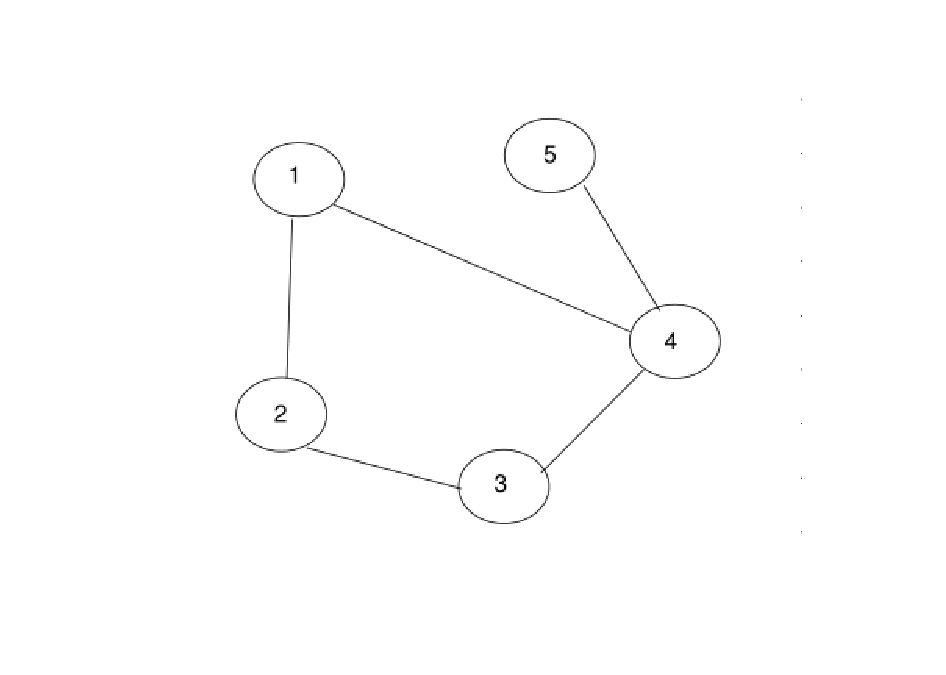
\includegraphics[width=1.8in]{delay/tuopu1.eps}}
            \subcomment[]{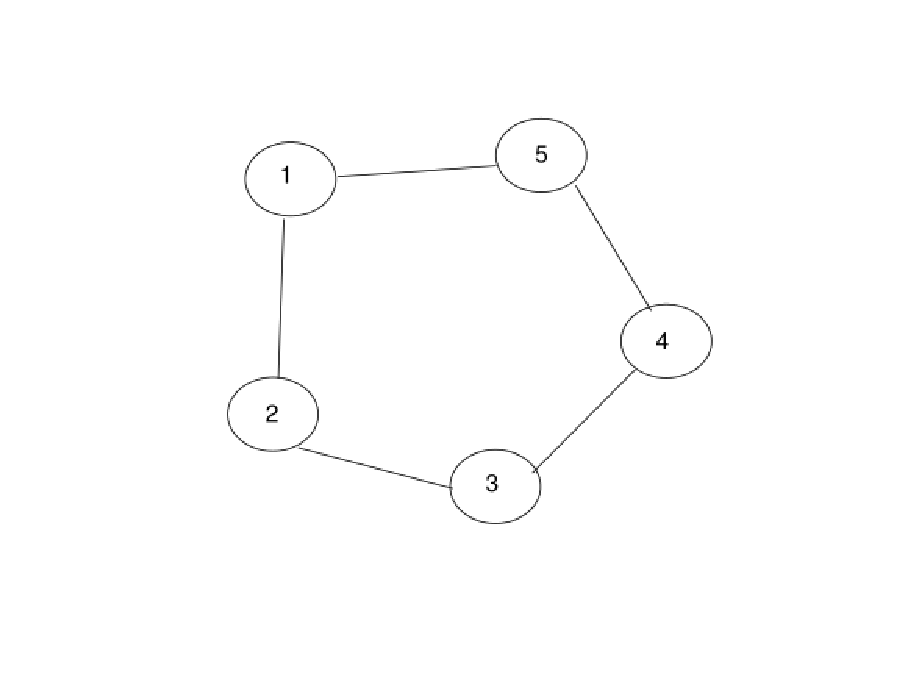
\includegraphics[width=1.8in]{delay/tuopu2.eps}}
            \subcomment[]{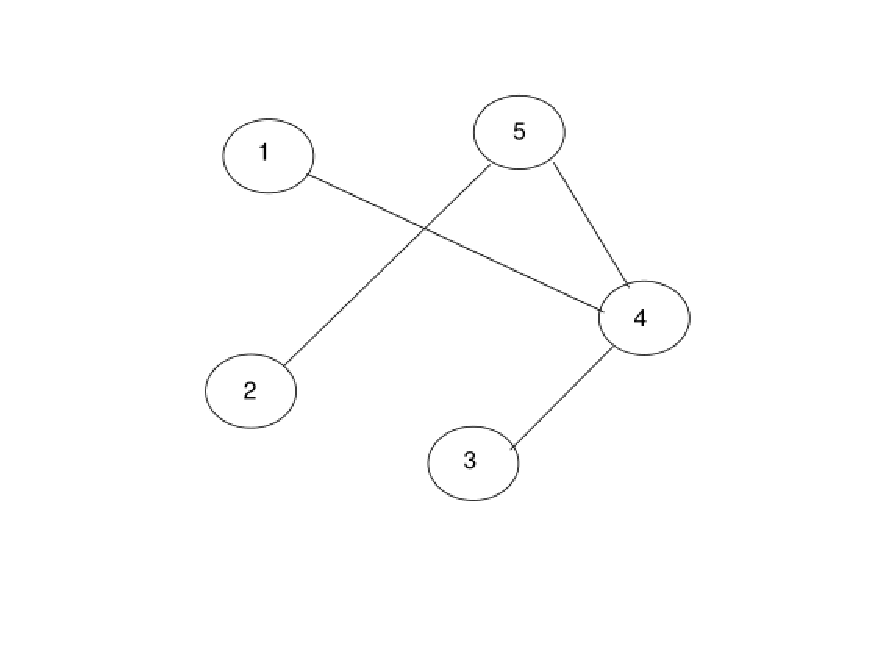
\includegraphics[width=1.8in]{delay/tuopu3.eps}}
     \end{center}
  \caption{网络系统在不同马氏链状态下可能的拓扑结构图.}\label{tuopu}
  \end{comment}
        本节给出一个数值的例子来印证定理的有效性. 考虑一个时滞的带有部分未知转移率的马尔可夫切换耦合的复杂网络, 该网络包含个节点, 每个节点包含个状态, 其动力学方程如下:
        \begin{comment}\label{numbersys}
           \nonumber \dot{x}_{i}(t)&=f(t,x_{i}(t),x_i(t-\tau))-c\sum^5_{j=1}l_{ij}(r_{t})[x_{j}(t_k)-x_{i}(t_{k})]+u_i(t),\\
            &\quad\quad t_{k}\leq t< t_{k+1} \quad i = 1,\cdots,5,
        \end{comment}
        其中是第个节点的状态向量; , . . 是有限状态空间上的马尔可夫链, 其部分未知转率矩阵如下:


    其中表示未知的转移率. 可以看出, 马尔可夫链的平均逗留时间服从参数为 的指数分布, 并且. 具体的演变过程见.
    可能的耦合结构如.
是随机发生控制器, 其定义如下:

其中是控制强度增益, 是相互独立的随机过程, 并且满足.
\begin{comment}[!htb]
\begin{minipage}[t]{0.48\linewidth}
\centering
\includegraphics[width=3.2in]{delay/comment1.eps}
\caption{马尔可夫链在转移概率矩阵下的状态切换.}
\label{Markovfig}
\end{minipage}~~
\begin{minipage}[t]{0.48\linewidth}
\centering
\includegraphics[width=3.2in]{delay/comment2.eps}
\caption{基于事件激发随机发生控制策略下, 时滞马氏系统  在参数下的节点状态向量轨道的变化情况.}
\label{state}
\end{minipage}
\end{comment}
\begin{comment}[!htb]
\begin{minipage}[t]{0.48\linewidth}
\centering
\includegraphics[width=3.2in]{delay/comment3.eps}
\caption{系统  总同步误差轨道.}
\label{totallerror}
\end{minipage}~~
\begin{minipage}[t]{0.48\linewidth}
\centering
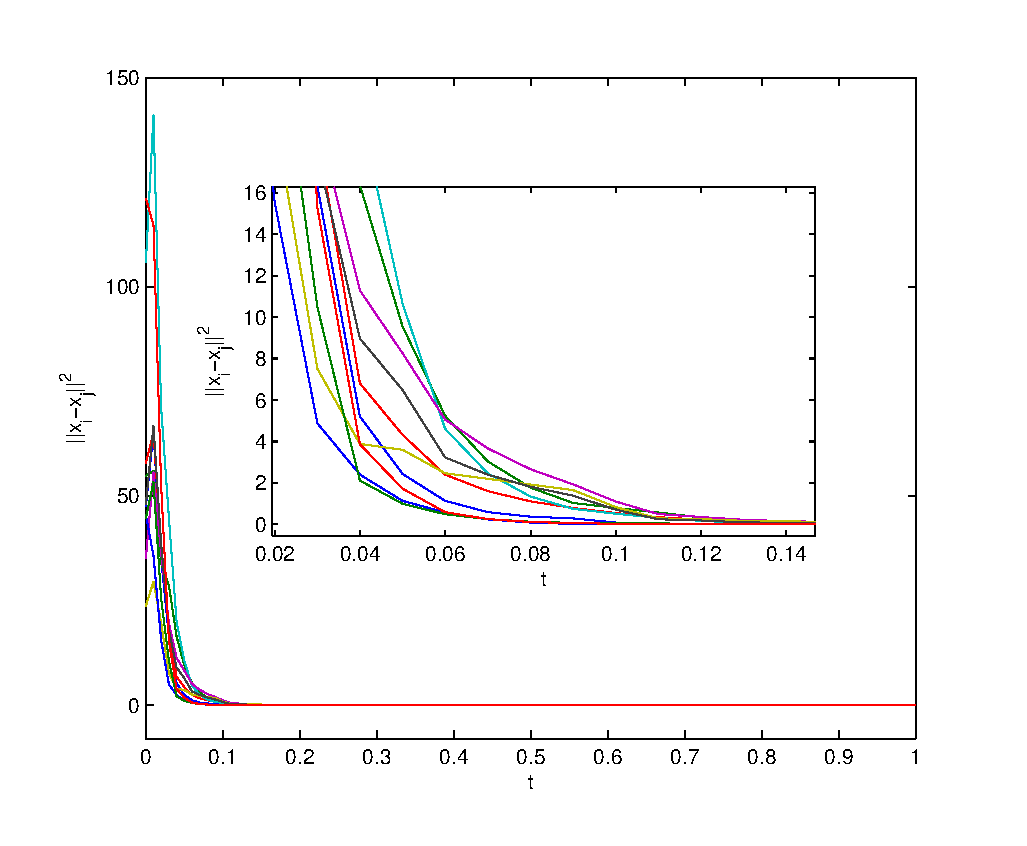
\includegraphics[width=3.2in,height=2.45in]{delay/xi-xj.eps}
\caption{不同节点间的状态差距演变过程.}\label{xixj}
\end{minipage}
\end{comment}

下面验证 与 的条件. 首先估计参数和使得满足, 根据的定义, 可以将 分解成时滞和非时滞两个部分: , 其中, . 于是函数所以可能的Jacobin矩阵为:
       \begin{comment}
        J_1=\left(
              \begin{array}{ccc}
                4.2299 &  9.78 & 0 \\
                1 & -1 & 1 \\
                0 &  -9.53 & 0 \\
              \end{array}
            \right),
        J_2=\left(
              \begin{array}{ccc}
                -2.1213 & 9.78 & 0 \\
                1 & -1 & 1 \\
                0 &  -9.53 & 0 \\
              \end{array}
            \right).
        \end{comment}
        对于任意和, 通过利用范数三角不等式性可得:
\begin{comment}[!htb]
\begin{minipage}[t]{0.48\linewidth}
\centering
\includegraphics[width=3.2in]{delay/comment4.eps}
\caption{策略误差的变化过程.}
\label{measurerror}
\end{minipage}~~
\begin{minipage}[t]{0.48\linewidth}
\centering
\includegraphics[width=3.2in,height=2.45in]{delay/comment5.eps}
\caption{Lyapunov-Krasovskii函数的变化过程.}\label{vt}
\end{minipage}
\end{comment}
        \begin{comment}
        &\quad\|f(t,x(t),x(t-\tau))-f(t,y(t),y(t-\tau))\|\\
        &\leq\|f_1(x(t))-f_1(y(t))\|+\|f_2(x(t-\tau))-f_2(y(t-\tau))\|\\
        &=\max\{\|J_1\|,\|J_2\|\}\|(x(t)-y(t))\|
        +\|-\eta\epsilon\sin(\nu
            x_1(t-\tau))+\eta\epsilon\sin(\nu y_1(t-\tau))\|\\
        &\leq\max\{\|J_1\|,\|J_2\|\}\|(x(t)-y(t))\|
        +|\eta\epsilon\nu|\|x_1(t-\tau)-y_1(t-\tau)\|\\
        &\leq\max\{\|J_1\|,\|J_2\|\}\|(x(t)-y(t))\|
        +|\eta\epsilon\nu|\|x(t-\tau)-y(t-\tau)\|.
        \end{comment}
       因此取可使得满足.

 其次, 选取以及, 则有和.
 最后, 选取, 则有, 以及. 容易证明, 对于任意且. 因此 和 的条件满足.

 利用欧拉法, 取步长为, 区间为. 通过MATLAB求解微分方程  并画出相应的变化图.

 展现了马尔可夫链在转移概率矩阵下的状态切换过程.  描绘了网络节点的各个状态随着时间演变的过程, 从该图可以看出, 不同节点间的同一状态趋于同步. 即, 在事件激发随机发生控制策略下, 时滞的马氏耦合系统  能够实现均方指数同步.

定义系统总误差如下:

系统总误差的演变过程参见. 各个节点轨道之间的距离差演变过程见. 从 和 可以看出, 网络系统  在很短时间内达到同步.  描述了测量误差的演变过程, 从该图中可以看到, 测量误差线与横轴的角度就是事件激发的时刻, 图中任意两个激发时刻之间都存在间隔, 且间隔没有随着时间的延长而减小. 这说明事件激发时刻间隔的正下界是存在的, 即Zeno现象不会发生.  展示了Lyapunov—Krasovskii 函数的变化情况以及与指数函数 的对比, 可以看出, 的收敛于零的速度比指数函数快一些, 因此该同步属于指数同步.

\section{小结}\label{con}
     本章利用集中式事件激发采样策略和随机发生控制方法研究了动力学时滞和带有马氏切换耦合复杂网络同步问题. 网络的马氏链的转移率矩阵是部分未知的, 并且孤立节点动力学受到时滞的影响. 通过利用Lyapunov稳定性理论以及随机分析知识, 本章得出了充分的同步条件并保证了Zeno现象不会发生. 最后, 给出了一些数值的例子来证实结论的有效性.
%%!Mode:: "Tex:UTF-8"


\chapter{基于事件激发采样带部分未知转移率和布朗运动的复杂网络同步问题}

        前面两章分别讨论了分散式和集中事件激发控制策略下不同网络模型的同步问题, 通过设计合适的事件激发控制规则, 利用随机过程理论以及稳定性定理, 给出网络同步的充分判据. 然而前面两章的网络模型没有考虑更为重要的随机因素, 即噪声干扰. 众所周知, 网络节点间的信号传输很容易遭受到噪声干扰, 特别是在计算机通信、保密通讯、输电网方面. 因此噪声是复杂网络同步研究不可忽略的因素. 本章在部分未知转移率的模式切换网络的基础上, 进一步讨论带有布朗运动的复杂网络同步问题. 并分别给出集中式和分散式两种事件激发规则.

\section{带布朗运动的一般网络模型}

        一个未受控制带有随机噪声干扰的马氏切换复杂网络模型如下:
        \begin{comment}\label{sys:gensys}
        \begin{split}
            \dot{x}_{i}(t)=f(x_{i}(t))-\rho(t)\sum^N_{j=1}l_{ij}(r_t)\Gamma[x_{j}(t)-x_{i}(t)+(\varepsilon_{ij}(t)\otimes\mathbf{1}_n)\xi_{ij}(t)],\quad i=1,2,\cdots,N,
        \end{split}
        \end{comment}
      其中是噪声强度, 是标准白噪声过程. 将网络  写成微分形式如下:
      \begin{comment}\label{sys-dt}
      \nonumber dx_{i}(t)=&\Big[f(x_{i}(t))-\rho(t)\sum^N_{j=1}l_{ij}(r_t)\Gamma(x_{j}(t)-x_{i}(t))\Big]dt\\
      &-\rho(t)\sum^N_{j=1}l_{ij}(r_t)\Gamma(\varepsilon_{ij}(t)\otimes\mathbf{1}_n)dw_{ij}(t), \quad i = 1,\cdots,N,
        \end{comment}
       其中是定义在上的标准布朗运动, 满足以及. 其他记号的含义在无特殊说明时与前文一致, 下同.

        下面给出当函数包含马尔可夫马过程和布朗运动时, 弱无穷小生成元算子求解方法.
        \begin{lem}\label{ET}{\rm\upcite{differential}}
        考虑一个定义在正无穷上, 初值为, 带有马尔可夫链和布朗运动形式的随机微分方程:

        其中

        记是定义在上关于二阶连续可微, 关于一阶可微的所有函数集. 如果.
        则关于从到上的弱无穷小生成元算子可以由下式给出:
        \begin{comment}
        \mathcal{L} V(t,x,r)=&V_t{(t,x,r)}+V_{x}{(t,x,r)}f(t,x,r) \notag \\
                 &+\frac{1}{2}\mathrm{tr}\big [\sigma(t,x,r)^\top V_{xx}\sigma(t,x,r)\big ]+\sum_{j=1}^M\gamma_{ij}V(t,x,j),
        \end{comment}
        其中\\$V_t{(t,x,r)}=\frac{\partial V(t,x,r) }{\partial t},V_{x}{(t,x,r)}=(\frac{\partial V(t,x,r) }{\partial x_1},
        \frac{\partial V(t,x,r) }{\partial x_2},\ldots,\frac{\partial V(t,x,r) }{\partial x_n}),V_{xx}{(t,x,r)}=(\frac{\partial^2(V(t,x,r)) }{\partial x_i \partial x_j})_{n\times n}.$
         \end{lem}

        为了方便叙述, 我们定义记号如下: , , , .

\section{集中式和分散式事件激发控制策略的同步分析}\label{result}
        集中式和分散式事件激发策略的区别在于, 集中式激发规则要求所有的节点在事件激发时刻同时更新状态, 而分散式激发规则中每个节点都有自己的激发规则. 这两种激发规则都是通过定义相应的激发函数, 当激发函数的阈值达到时, 事件就被激发, 节点的信息得到更新.
\subsection{基于集中式事件激发控制的网络模型以及同步分析}\label{centralized}
        集中式事件激发控制策略指的是根据节点的状态信息构造统一的事件激发函数, 所有节点都遵循该激发函数进行信息的更新. 设置集中式事件激发控制输入 如下:
        \begin{comment}
            u_i(t_k)=-\epsilon\rho(t)d_{i}(r_{t})\Gamma[x_{i}(t_{k})-s(t_{k})]
        \end{comment}
        这里的控制输入与第 \ref{chapternonline} 章的控制输入  不同在于此处的控制输入是线性的.

        网络 ) 在上述控制器控制下可转化为如下形式:
        %consider the discontinuous diffusing complex network under centralized event triggered strategy as following, the  centralized event-triggered function will be designed to impel this network to realize exponentially synchronization.
        \begin{comment}\label{sys_cen}
        \nonumber dx_{i}(t)&=\Big[f(x_{i}(t))-\rho(t)\sum^N_{j=1}l_{ij}(r_{t})\Gamma(x_{j}(t_k)-x_{i}(t_{k}))
        +u_i(t)\Big]dt-\rho(t)R_i(t)dw_{i}(t),\\
         &\quad t_{k}\leq t< t_{k+1}, \quad i = 1,\cdots,N,
        \end{comment}
        其中, , 是严格递增的集中式事件激发时刻序列.

        定义节点测量误差. 因为, 所以网络系统  可以表示成误差系统的形式:
        \begin{comment}
            \nonumber d{e}_{i}(t)=&\Big[f(x_{i}(t))-f(s(t))-\rho(t)\sum^N_{j=1}l_{ij}(r_{t})\Gamma(\delta_j(t)+e_j(t))
            -\epsilon\rho(t)d_{i}(r_{t})\Gamma(\delta_i(t)+e_i(t)\\
                &+s(t)-s(t_k))\Big]dt-\rho(t)R_i(t)dw_{i}(t), \quad t_{k}\leq t< t_{k+1}, \quad i = 1,\cdots,N.
        \end{comment}
        利用Kronecker积的性质, 上式可以改成如下:
        \begin{comment}\label{tallerr}
         \nonumber  de(t)=&\Big[f(e(t))-\rho(t)[L(r_t)\otimes\Gamma](\delta(t)+e(t))
        -\epsilon\rho(t)[D(r_t)\otimes\Gamma](\delta(t)+e(t)+\hat{s}(t))\Big]dt\\
        &-\rho(t)\Sigma(t)dw(t),\quad t_{k}\leq t< t_{k+1}, \quad i = 1,\cdots,N.
        \end{comment}
        其中, , , , ,

        定义集中式事件激发函数如下:
        \begin{comment}\label{trig-f}
            g^c(t)=(1+\epsilon)\|\delta(t)\|^2+\epsilon\|\hat{s}(t)\|^2-\frac{\xi^2\underline{q}^2}{4(\bar{\lambda}^2+2\epsilon)c^2\bar{q}^2\bar{\gamma}^2}\|e(t)\|^2
        \end{comment}
        \begin{rem}
        在时刻, 如果达到阈值, 那么事件就被激发, 新的事件激发时刻被确定, 即. 此时所有的节点状态和控制输入都要更新至该时刻的信息. 此后直到下一次事件激发.
        \end{rem}
        \begin{thm}\label{thm:cen}
            如果属于, 噪声强度满足, 并且存在正数, 使得对所有, 下式不等式成立:
            \begin{comment}\label{ce-condiction}
            \left\{
            \begin{commented}
                  &(\bar{\delta}+\chi_u)I_N-c\underline{\gamma}(L(u)+\epsilon D(u))\leq0,\\
                  &\pi_v-a_u\leq0, \quad \text{if}\quad v\neq u, v\in S^u_2,\\
                  &\pi_v-a_u\geq0, \quad \text{if} \quad v= u, v\in S^u_2,
            \end{commented}
            \right.
            \end{comment}
           其中, , , 那么在事件激发函数  下, 网络系统  可以实现均方指数同步.
        \end{thm}
        \begin{proof}
        定义Lyapunov-Krasovskii函数为
        \begin{comment}
        V(t)=\frac{1}{2}\pi_{r_t}e^\top(t)[I_N\otimes Q]e(t).
        \end{comment}
        当时, 根据可得
        \begin{comment}\label{dVt}
        dV(t)&=\mathcal{L}V(t)dt+\rho(t)\pi_ue^\top(t)(I_N\otimes Q)\Sigma(t)dw(t),
        \end{comment}
        其中
        \begin{comment}\label{LV}
        \nonumber\mathcal{L}V(t)&=\pi_ue^\top(t)[I_N\otimes Q]\Big\{\tilde{f}(e(t))-\rho(t)\left[L(u)\otimes\Gamma\right](e(t)+\delta(t))\\
        \nonumber &\quad-\epsilon\rho(t)[D(u)\otimes\Gamma](\delta(t)+e(t)+\hat{s}(t))\Big\}\\
        \nonumber &\quad+\frac{1}{2}\pi_u\rho^2(t)\text{tr}[(I_N\otimes Q)\Sigma(t)\Sigma^\top(t)]+\frac{1}{2}\sum_{v=1}^{m}q_{uv}\pi_ve^\top(t)[I_N\otimes Q]e(t)\\
        \nonumber&\leq\pi_ue^\top(t)[I_N\otimes Q]\tilde{f}(e(t))-\pi_u\rho(t)\underline{\gamma}e^\top(t)[L(u)\otimes Q]e(t)\\
        \nonumber&\quad-\pi_u\rho(t)e^\top(t)[L(u)\otimes Q\Gamma]\delta(t)-\pi_u\epsilon\rho(t)e^\top(t)[D(u)\otimes Q\Gamma]\delta(t)\\
        \nonumber &\quad-\pi_u\epsilon\rho(t)\underline{\gamma}e^\top(t)[D(u)\otimes Q]e(t)-\pi_u\epsilon\rho(t)e^\top(t)[D(u)\otimes Q\Gamma]\hat{s}(t)\\
        &\quad+\frac{1}{2}\pi_u\rho^2(t)\text{tr}[(I_N\otimes Q)\Sigma(t)\Sigma^\top(t)]+\frac{1}{2}\sum_{v=1}^{m}q_{uv}\pi_ve^\top(t)[I_N\otimes Q]e(t).
        \end{comment}
        因为属于, 所以
        \begin{comment}
        \nonumber e^\top(t)[I_N\otimes Q]\tilde{f}(e(t))&\leq-\xi e^\top(t)[I_N\otimes Q]e(t)+e^\top(t)[I_N\otimes Q\Delta]e(t)\\
        &\leq(\bar{\delta}-\xi)e^\top(t)[I_N\otimes Q]e(t).
        \end{comment}
        通过利用, 可得
        \begin{comment}
        \nonumber-e^\top(t)[L(u)\otimes Q\Gamma]\delta(t)&\leq\frac{\mu}{2}e^\top(t)[L(u)L(u)^\top\otimes Q^2\Gamma^2]e(t)+\frac{1}{2\mu}\delta^\top(t)\delta(t)\\
        &\leq\frac{\mu}{2}\bar{\lambda}^2\bar{q}^2\bar{\gamma}^2 e^\top(t)e(t)+\frac{1}{2\mu}\delta^\top(t)\delta(t).
        \end{comment}
        其中, , .
        \begin{comment}
        \nonumber-e^\top(t)[D(u)\otimes Q\Gamma]\delta(t)&\leq\frac{\mu}{2}e^\top(t)[D(u)D(u)^\top\otimes Q^2\Gamma^2]e(t)+\frac{1}{2\mu}\delta^\top(t)\delta(t)\\
        &\leq\frac{\mu}{2}\bar{q}^2\bar{\gamma}^2 e^\top(t)e(t)+\frac{1}{2\mu}\delta^\top(t)\delta(t).
        \end{comment}
        类似地,
        \begin{comment}
        \nonumber-e^\top(t)[D(u)\otimes Q\Gamma]\hat{s}(t)&\leq\frac{\mu}{2}e^\top(t)[D(u)D(u)^\top\otimes Q^2\Gamma^2]e(t)+\frac{1}{2\mu}\delta^\top(t)\hat{s}(t)\\
        &\leq\frac{\mu}{2}\bar{q}^2\bar{\gamma}^2e^\top(t)e(t)+\frac{1}{2\mu}\hat{s}^\top(t)\hat{s}(t).
        \end{comment}
        根据的定义可得. 因此, .
        \begin{comment}\label{tr}
        \nonumber\text{tr}[(I_N\otimes Q)\Sigma(t)\Sigma^\top(t)]&\leq\text{tr}[I_N\otimes Q]\text{tr}[\Sigma(t)\Sigma^\top(t)]\\
        \nonumber&\leq Nq\sum_{i=1}^N\text{tr}[R_i(t)R_i^\top(t)]\\
        &=Nqh(t),
        \end{comment}
        其中, .
        根据以及条件 可得
        \begin{comment}\label{quv}
        \nonumber e^\top(t)\sum_{v=1}^{m}q_{uv}\pi_v[I_N\otimes Q]e(t)&=e^\top(t)\Big[\sum_{v=1}^{m}q_{uv}(\pi_v-a_u)(I_N\otimes Q)\Big]e(t)\\
        \nonumber&=e^\top(t)\Big\{\Big[\sum_{v\in S_1^u}q_{uv}(\pi_v-a_u)+\sum_{v\in S_2^u}q_{uv}(\pi_v-a_u)\Big](I_N\otimes Q)\Big\}e(t)\\
        &\leq 2\chi_u\pi_ue^\top(t)[I_N\otimes Q]e(t),
        \end{comment}
        其中.

        又因为噪声强度满足, 所以.
        根据 以及可得
        \begin{comment}\label{ELVt}
        \nonumber E\mathcal{L}V(t)\leq&-\pi_u\xi e^\top(t)[I_u\otimes Q]e(t)+\pi_ue^\top(t)[((\bar{\delta}+\chi_u)I_N-c\underline{\gamma}(L(u)+\epsilon D(u)))\otimes Q]e(t)\\
        \nonumber&+\frac{1}{2}(\bar{\lambda}^2+2\epsilon)\pi_uc\bar{q}^2\bar{\gamma}^2\mu e^\top(t)e(t)
        +(1+\epsilon)\pi_uc\frac{1}{2\mu}\delta^\top(t)\delta(t)\\
        &+\pi_u\epsilon c\frac{1}{2\mu}\hat{s}^\top(t)\hat{s}(t)+\frac{1}{2}\pi_uc^2Nqh(t).
        \end{comment}

        对式  两边同时取期望, 由于, 结合式 、式  以及条件  可得:
        \begin{comment}\label{EdVt}
        \nonumber \frac{d\mathrm{E}V(t)}{dt}\leq&-\pi_u\xi e^\top(t)[I_u\otimes Q]e(t)+\frac{1}{2}(\bar{\lambda}^2+2\epsilon)\pi_uc\bar{q}^2\bar{\gamma}^2\mu e^\top(t)e(t)\\
        \nonumber&+(1+\epsilon)\pi_uc\frac{1}{2\mu}\delta^\top(t)\delta(t)+\pi_u\epsilon c\frac{1}{2\mu}\hat{s}^\top(t)\hat{s}(t)+\frac{1}{2}\pi_uc^2Nqh(t)\\
        \nonumber\leq&-\xi \mathrm{E}V(t)+\frac{1}{2}\pi_uc^2Nqh(t)+\frac{\pi_u}{2}[-\xi\underline{q}+(\bar{\lambda}^2
        +2\epsilon)c\bar{q}^2\bar{\gamma}^2\mu]e^\top(t)e(t)\\
        &+\frac{\pi_u}{2\mu}c[(1+\epsilon)\delta^\top(t)\delta(t)+\epsilon\hat{s}^\top(t)\hat{s}(t)].
        \end{comment}
        由于上式对任意都成立, 故可取, 此时有
        \begin{comment}
        -\xi\underline{q}+(\bar{\lambda}^2+2\epsilon)c\bar{q}^2\bar{\gamma}^2\mu
        =-\frac{c}{\mu}\frac{\xi^2\underline{q}^2}{4(\bar{\lambda}^2+2\epsilon)c^2\bar{q}^2\bar{\gamma}^2}.
        \end{comment}
        在事件激发函数  下, 式  可以转化为
        \begin{comment}
        \frac{d\mathrm{E}V(t)}{dt}\leq-\xi \mathrm{E}V(t)+\frac{1}{2}\pi_uc^2Nqh(t).
        \end{comment}
        根据比较原理可得,
        \begin{comment}
        \mathrm{E}V(t)\leq V(0)e^{-\xi t}+\frac{1}{2}\pi_uc^2Nq\int_0^th(s)e^{-\xi(t-s)}ds.
        \end{comment}

        因为, 故对任意给定, 存在使得. 因此, 对任意, 有
        \begin{comment}
        \nonumber\int_0^th(s)e^{-\xi(t-s)}ds&=\int_0^\delta h(s)e^{-\xi(t-s)}ds+\int_\delta^th(s)e^{-\xi(t-s)}ds\\
        \nonumber&\leq e^{-\xi(t-\delta)}\int_0^\delta h(s)ds+\int_\delta^th(s)ds\\
        \nonumber&\leq e^{-\xi(t-\delta)}\int_0^\infty h(s)ds+\int_\delta^\infty h(s)ds\\
        &\leq e^{-\xi(t-\delta)}\int_0^\infty h(s)ds+\eta.
        \end{comment}
        因此, 根据的定义可得. 于是, 对任意, . 即网络系统  可以实现均方同步.
        \end{proof}

\subsection{基于分散式事件激发控制的网络模型以及同步分析}\label{decentralized}
        在集中式事件激发策略中, 当激发函数  达到阈值的时候, 所有的节点此刻同时发生更新, 这将会导致节点间的信息传输频繁. 对于大规模的复杂网络, 信息的频繁传输使得的网络通信不安全, 并且加大通讯负荷. 为了减少信号传输的频率, 分散式的事件激发控制策略是一个很好的选择. 在分散式事件激发策略中, 每一个节点都有特殊的激发函数, 并且该激发函数函数只依赖于自身节点的状态信息. 该策略下受控的网络微分方程如下:
        \begin{comment}\label{sys_decen}
        \begin{split} dx_{i}(t)=&\Big[f(x_{i}(t))-\rho(t)\sum^N_{j=1}l_{ij}(r_{t})\Gamma(x_{j}(t^j_{k'})-x_{i}(t^i_{k}))+u_i(t)\Big]dt\\
         &-\rho(t)R_i(t)dw_{i}(t),\quad t^i_{k}\leq t< t^i_{k+1}, \quad i = 1,\cdots,N,
        \end{split}
        \end{comment}
       其中是严格递增的序列, 它表示节点的事件激发时刻; ; 控制输入定义如下:
        \begin{comment}
            u_i(t^i_k)=-\epsilon\rho(t)d_{i}(r_{t})\Gamma[x_{i}(t^i_{k})-s(t^i_{k})].
        \end{comment}

        由于每个节点激发时刻不一致, 因此测量误差形式为. 若没有特殊说明, 其他的记号与 \ref{centralized} 的定义一样. 类似于 \ref{centralized}, 网络系统  可以改写成误差系统的形式:
        \begin{comment}\label{deeit}
            \nonumber d{e}_{i}(t)=&\Big[f(x_{i}(t))-f(s(t))-\rho(t)\sum^N_{j=1}l_{ij}(r_{t})\Gamma(\delta_j(t)+e_j(t))
            -\epsilon\rho(t)d_{i}(r_{t})\Gamma(\delta_i(t)\\
                &+e_i(t)+s(t)-s(t_k))\Big]dt-\rho(t)R_i(t)dw_{i}(t), \quad t^i_{k}\leq t< t^i_{k+1}, \quad i = 1,\cdots,N.
        \end{comment}
        通过利用 Kronecker 积的性质,
        网络系统  可以改写为如下:
        \begin{comment}
        \nonumber de(t)=&\big[f(e(t))-\rho(t)[L(r_t)\otimes\Gamma](\delta(t)+e(t))
        -\epsilon\rho(t)[D(r_t)\otimes\Gamma](\delta(t)+e(t)+\hat{s}(t))\big]dt\\
        &-\rho(t)\Sigma(t)dw(t), \quad t^i_{k}\leq t< t^i_{k+1}, \quad i = 1,\cdots,N,
        \end{comment}

        不同于集中式激发策略, 关于节点的分散式激发函数定义为如下:
        \begin{comment}\label{detrig-f}
            g^i(t)=(1+\epsilon)\|\delta_i(t)\|^2+\epsilon\|\hat{s}_i(t)\|^2-\frac{\xi^2\underline{q}^2}{4(\bar{\lambda}^2+2\epsilon)c^2\bar{q}^2\bar{\gamma}^2}\|e_i(t)\|^2,
        \end{comment}
        %这里.
        \begin{rem}
            在分散式事件激发策略中, 当分散式激发函数将要达到阈值的时候, 每个节点更新自己的状态信息, 同时发送此时的状态信息给邻居节点. 在任意时刻, 事件激发函数 都是负的. 这是因为在事件激发点处, 测量误差等于. 也就是说激发函数在事件激发时刻是右连续的, 激发时刻是激发函数的跳跃间断点.
        \end{rem}
        \begin{thm}\label{thm:decen}
            如果属于, 噪声强度满足, 并且存在正数, 使得对所有, 下式不等式成立:
            \begin{comment}\label{de-condiction}
            \left\{
            \begin{commented}
                  &(\bar{\delta}+\chi_u)I_N-c\underline{\gamma}(L(u)+\epsilon D(u))\leq0,\\
                  &\pi_v-a_u\leq0, \quad \text{if},\quad v\neq u, v\in S^u_2,\\
                  &\pi_v-a_u\geq0, \quad \text{if}, \quad v= u, v\in S^u_2,
            \end{commented}
            \right.
            \end{comment}
        其中, 则在事件激发函数  下, 网络系统  均方同步到.
        \end{thm}
        \begin{proof}
        在本定理的证明中, 使用定理  证明给出的 Lyapunov-Krasovskii 函数, 类似于 -, 有
        \begin{comment}\label{deEdVt}
        \nonumber \frac{dEV(t)}{dt}\leq&-\xi EV(t)+\frac{1}{2}\pi_uc^2Nqh(t)+\frac{\pi_u}{2}[-\xi\underline{q}+(\bar{\lambda}^2
        +2\epsilon)c\bar{q}^2\bar{\gamma}^2\mu]e^\top(t)e(t)\\
        \nonumber&+\frac{\pi_u}{2\mu}c[(1+\epsilon)\delta^\top(t)\delta(t)+\epsilon\hat{s}^\top(t)\hat{s}(t)]\\
        \nonumber=&-\xi EV(t)+\frac{1}{2}\pi_uc^2Nqh(t)+\frac{\pi_u}{2}\sum_{i=1}^N\bigg\{[-\xi\underline{q}+(\bar{\lambda}^2
        +2\epsilon)c\bar{q}^2\bar{\gamma}^2\mu]e_i^\top(t)e_i(t)\\
        &+\frac{c}{\mu}[(1+\epsilon)\delta_i^\top(t)\delta_i(t)+\epsilon\hat{s}_i^\top(t)\hat{s}_i(t)]\bigg\}.
        \end{comment}

        由于  对任意都成立, 因此可以选择. 根据分散式激发函数 , 在式  中的求和项小于或等于. 因此有
        \begin{comment}
            \frac{dEV(t)}{dt}\leq-\xi EV(t)+\frac{1}{2}\pi_uc^2Nqh(t).
        \end{comment}

        类似于  的讨论, 可以得出, 对任意, 成立, 于是根据三角不等式可得, 对任意, . 于是根据定义 , 网络系统  在均方意义下同步到.
        \end{proof}

\section{数值模拟}\label{simulate}
    为了验证理论结果的有效性, 本节给出一个数值仿真例子. 考虑一个个节点的马尔可夫切换网络模型:
\begin{comment}
        \begin{split}\label{exmsystem}
            \dot{x}_{i}(t)=f(x_{i}(t))-\rho(t)\sum^5_{j=1}l_{ij}(r_t)\Gamma[x_{j}(t)-x_{i}(t)+(\varepsilon_{ij}(t)\otimes\mathbf{1}_n)\xi_{ij}(t)],\quad i=1,2,\cdots,5,
        \end{split}
        \end{comment}
    其中, ,
    这里. 从节点自身动力学可以看出, 每个节点都是线性耦合的 Chua's 电路\upcite{chuacircuits}. 选择参数, 那么此时自身节点动力学具有双混沌吸引子. 对任意是标准白噪声, , 以及.
    \begin{comment}
  % Requires \usepackage{graphicx}
     \begin{center}
            \subcomment[]{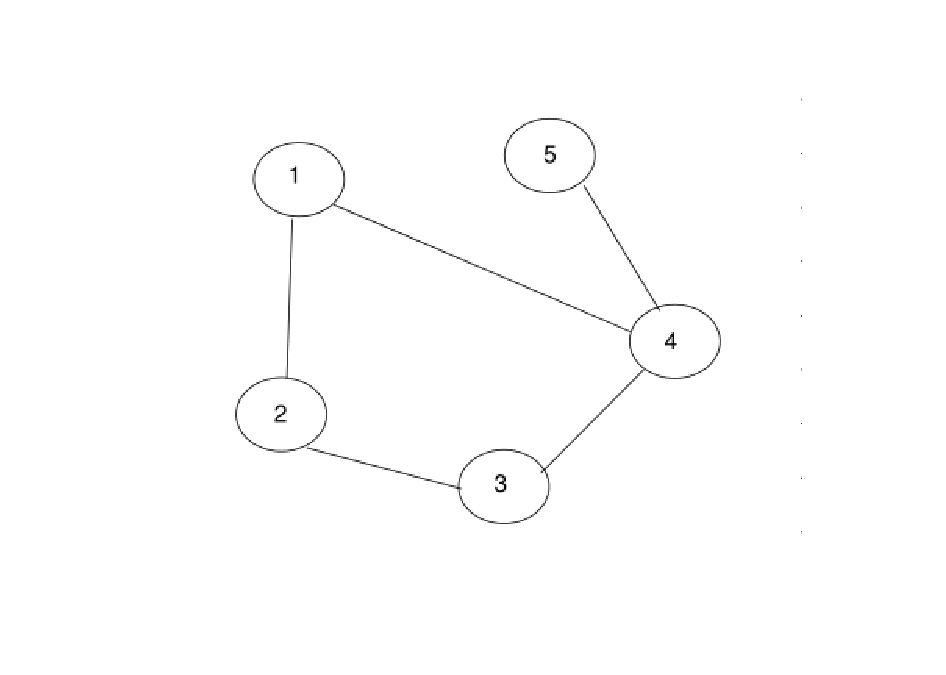
\includegraphics[width=1.8in]{delay/tuopu1.eps}}
            \subcomment[]{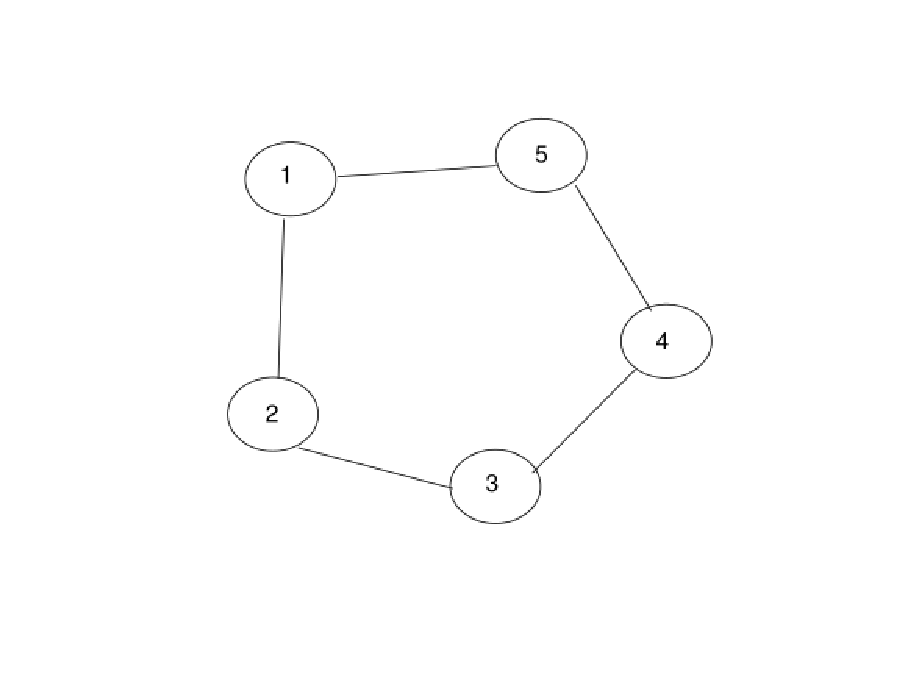
\includegraphics[width=1.8in]{delay/tuopu2.eps}}
            \subcomment[]{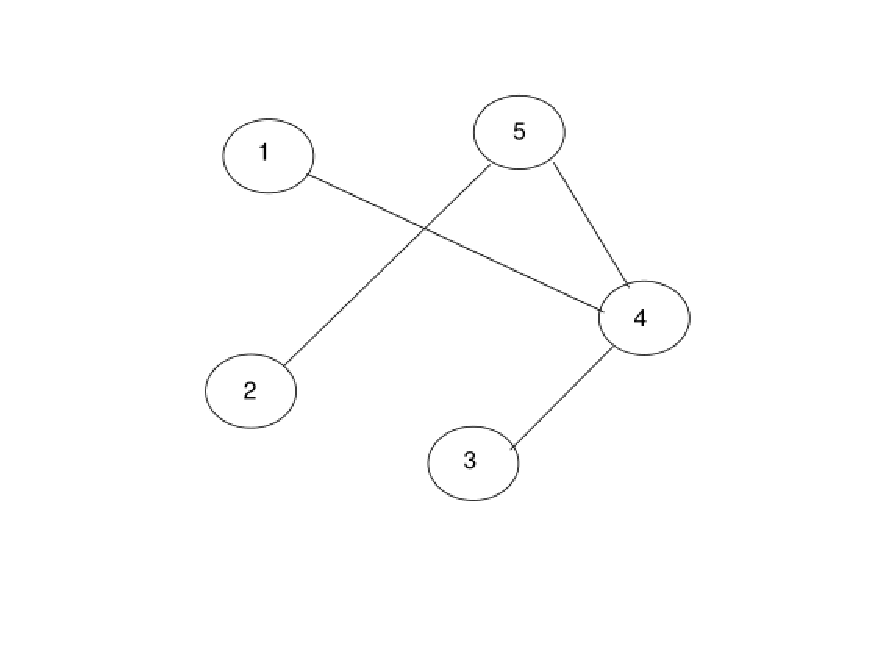
\includegraphics[width=1.8in]{delay/tuopu3.eps}}
     \end{center}
  \caption{网络系统在不同马氏链状态下可能的拓扑结构图.}\label{tuopu}
  \end{comment}
\begin{comment}[!htb]
\begin{minipage}[t]{0.48\linewidth}\centering
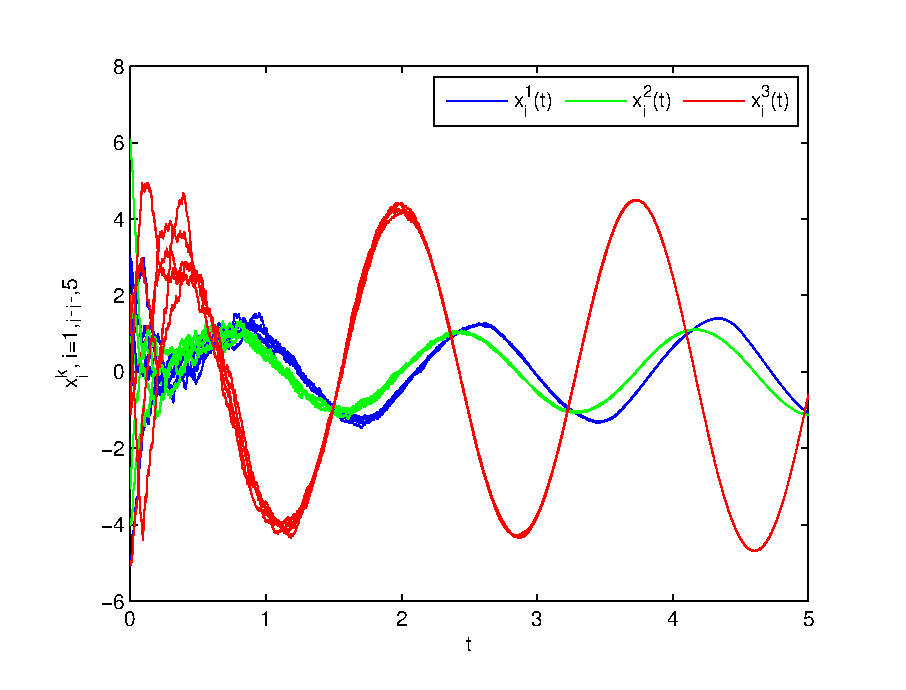
\includegraphics[width=3.2in]{noise/cestate.eps}\caption{在集中式激发策略  下, 节点各个状态随时间演变图.}\label{cefig}
\end{minipage}~~
\begin{minipage}[t]{0.48\linewidth}\centering
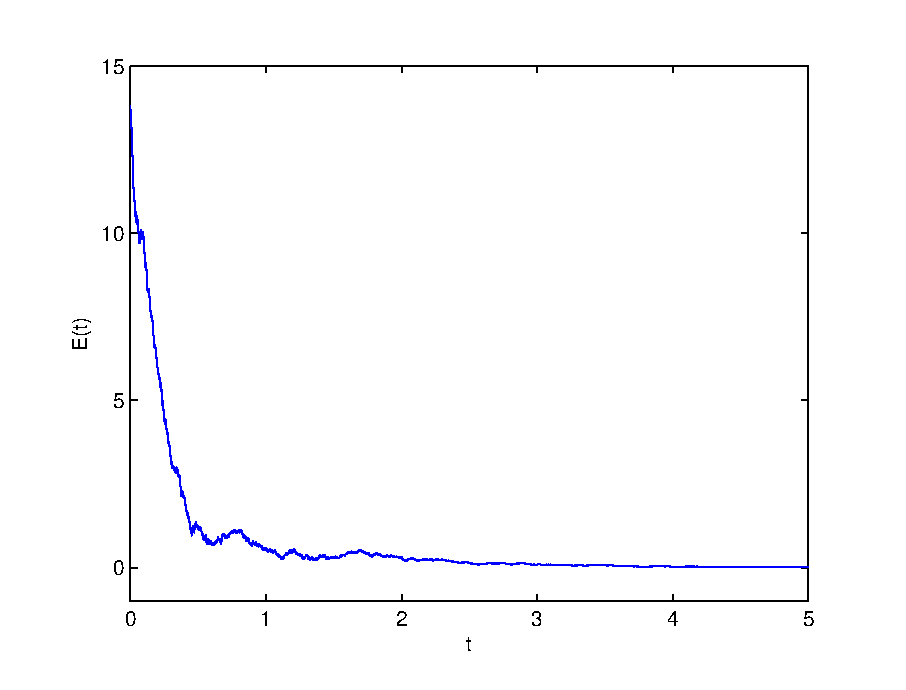
\includegraphics[width=3.2in,height=2.45in]{noise/ceEt.eps}\caption{在集中式激发策略  下, 系统总误差随时间演变图.}\label{ceEt}
\end{minipage}
\end{comment}
   是定义在有限状态空间上的马尔可夫链, 其每个状态的平均逗留时间服从参数为的指数分布, 并且转移率是部分未知的, 转移率矩阵如下:

    其中表示未知转移率.

    复杂网络所有可能的拓扑结构如. 相应的控制节点集为, 和是相应马尔可夫链状态下的牵制节点集.
\begin{comment}[!htb]
\begin{minipage}[t]{0.48\linewidth}\centering
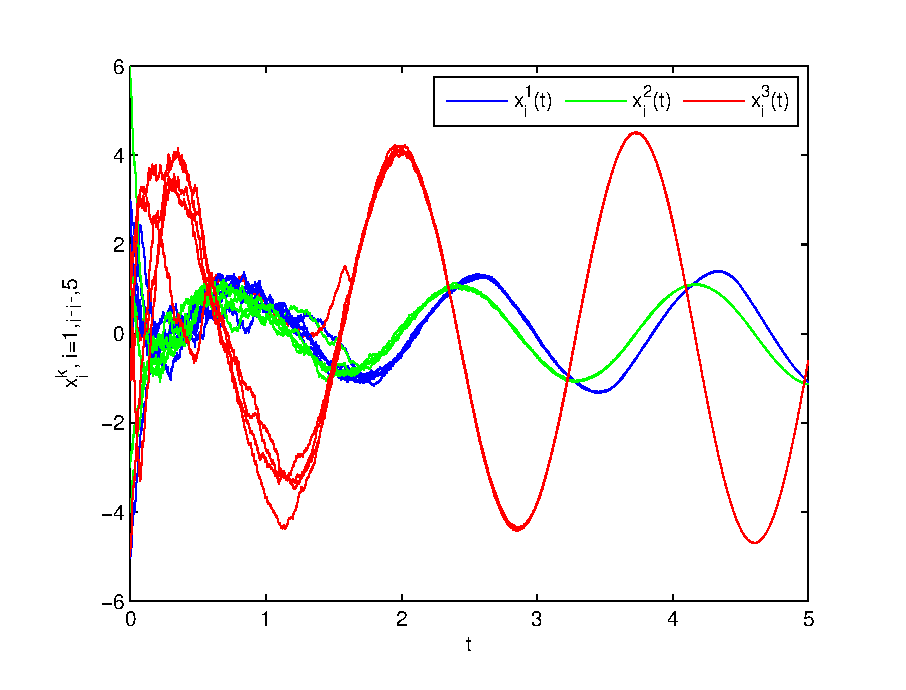
\includegraphics[width=3.2in]{noise/destate.eps}\caption{在分散式激发策略  下, 节点各个状态随时间演变图.}\label{defig}
\end{minipage}~~
\begin{minipage}[t]{0.48\linewidth}\centering
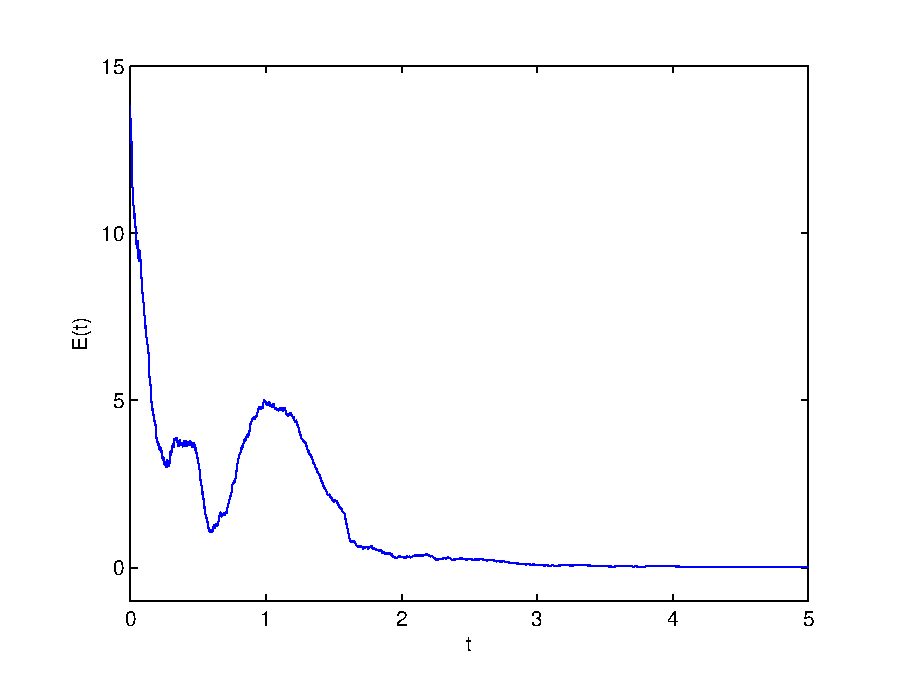
\includegraphics[width=3.2in,height=2.45in]{noise/deEt.eps}\caption{在分散式激发策略  下, 系统总误差随时间演变图.}\label{deEt}
\end{minipage}
\end{comment}

    选取参数, . 为了估计 QUAD 条件中的参数, 这里先求的 Jacobin 矩阵如下:
        \begin{comment}
        J_1=\left(
              \begin{array}{ccc}
                3.0318 & 9.78 & 0 \\
                1 & -1 & 1 \\
                0 & -14.97 & 0 \\
              \end{array}
            \right),
        J_2=\left(
              \begin{array}{ccc}
                -2.445 & 9.78 & 0 \\
                1 & -1 & 1 \\
                0 & -14.97 & 0 \\
              \end{array}
            \right).
        \end{comment}
        通过计算可知, 所有的 Jacobin 矩阵的最大特征值为. 于是可得. 因为是正数, 故可取, 此时.

    为了保证 和 的条件满足, 这里选取, 以及.节点的初值状态, , , , , 以及.
    定义系统同步误差为


    网络系统的微分方程求解方法利用的是欧拉迭代法, 步长为, 迭代时间为, 数值解的结果以图片的形式给出, 见.

    从 和 可以看出, 基于集中式事件激发策略  下, 复杂网络系统的每一个节点每一维度的状态向量随着时间的演变慢慢地趋于同步, 并且系统同步误差从迅速递减到. 同样的, 在分散式事件激发策略下,  和 展示了复杂网络系统各个节点的状态随着时间的演变趋于一致, 并且系统系统误差以较大的速度收敛于.
    \begin{comment}[!htb]
\begin{minipage}[t]{0.48\linewidth}\centering
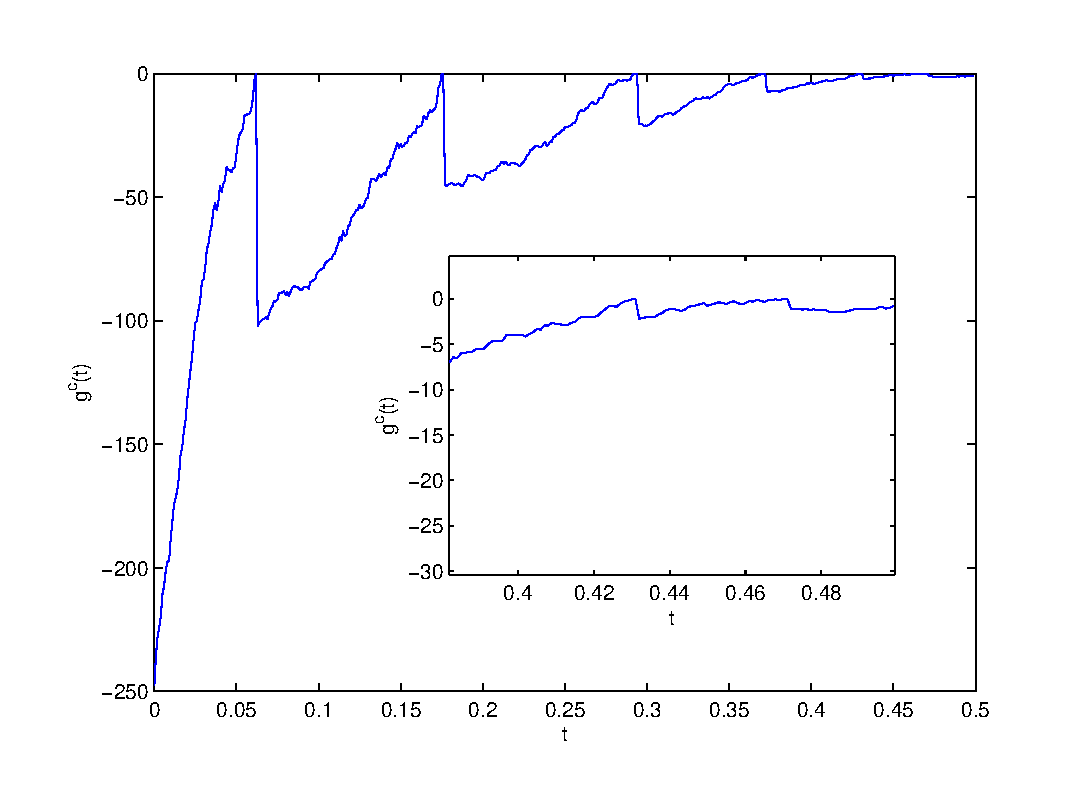
\includegraphics[width=3.2in]{noise/gct.eps}\caption{在分散式激发策略  下, 系统总测量误差图.}\label{gt}
\end{minipage}~~
\begin{minipage}[t]{0.48\linewidth}\centering
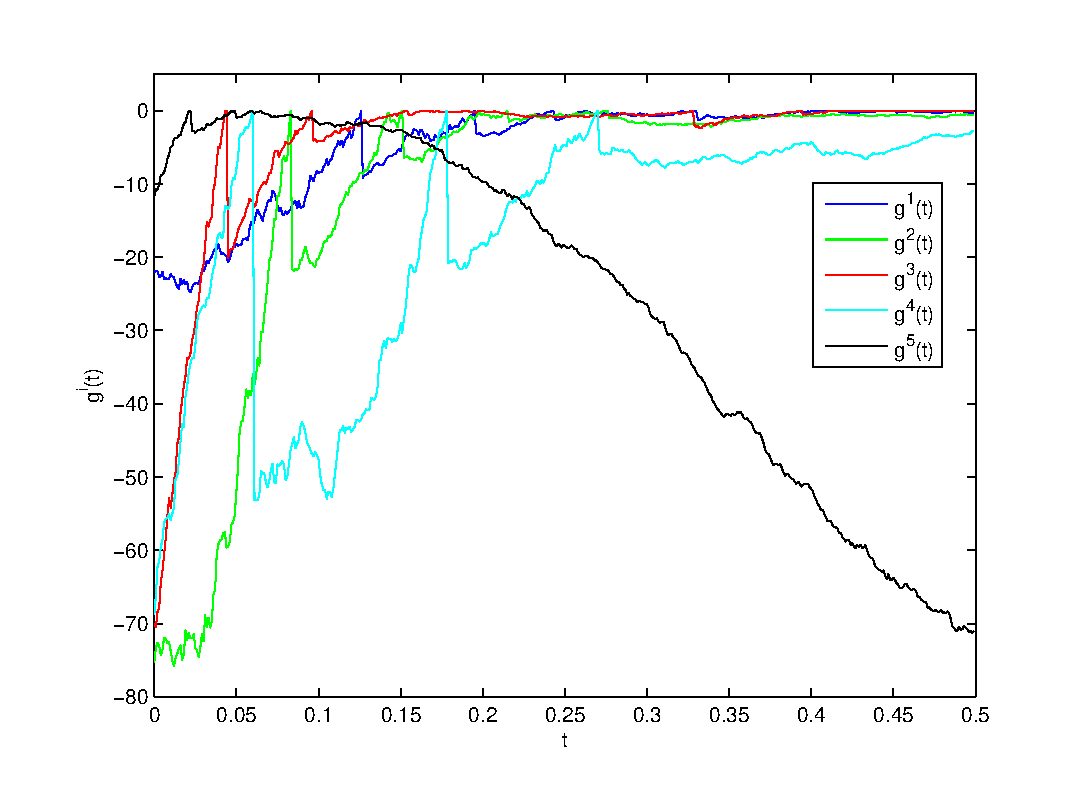
\includegraphics[width=3.2in,height=2.45in]{noise/git.eps}\caption{在分散式激发策略  下, 各个节点的策略误差图.}\label{degt}
\end{minipage}
\end{comment}
\begin{comment}[!htb]
\begin{minipage}[t]{0.48\linewidth}\centering
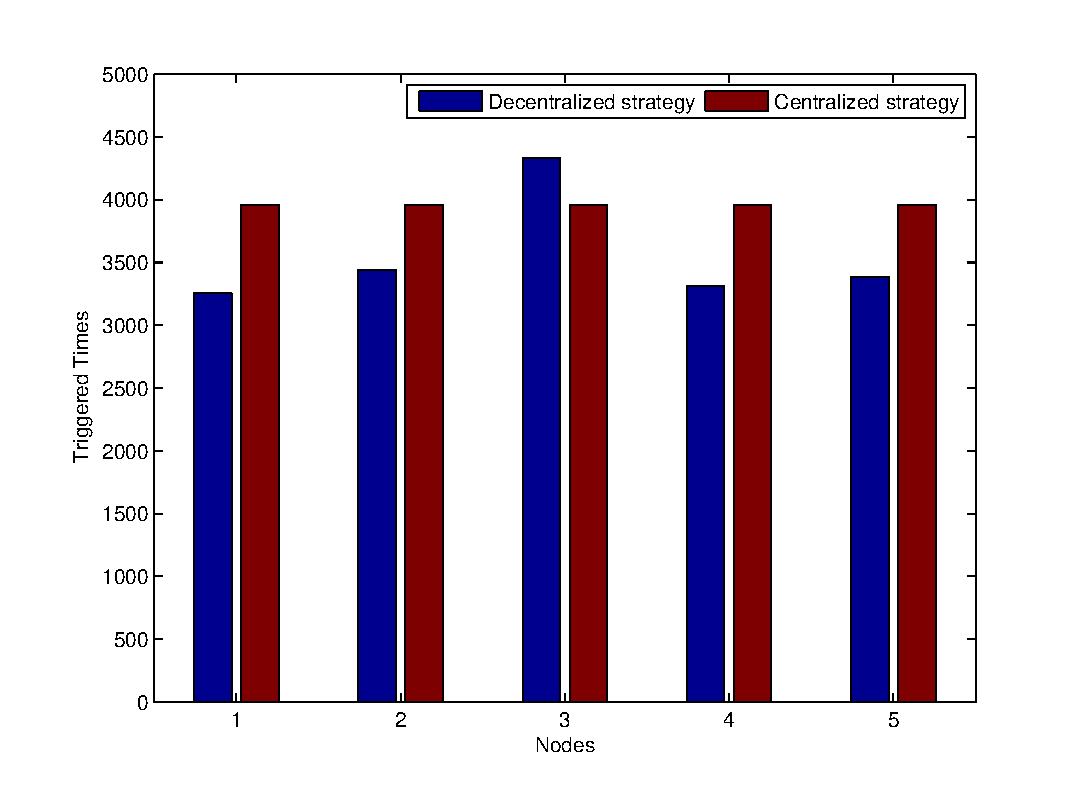
\includegraphics[width=3.2in]{noise/trigger.eps}\caption{在集中式激发策略  和分散式激发策略 下, 节点激发次数对比图.}\label{tritimes}
\end{minipage}
\end{comment}

    为了更好的展现事件激发的过程,  和 给分别出了在集中式事件激发策略和分散式事件激发策略下的激发函数的变量情况. 从图中可以看到, 集中式和分散式的激发函数值都是负数. 当激发函数是左极限等于零的时候, 此时事件被激发, 测量误差就等于零, 从而使得激发函数的值就等于同步误差的相反数, 此后, 测量误差有开始慢慢的增大至同步误差时, 事件就再一次被激发. 因此事件激发函数是具有周期缩短且函波峰逐渐平缓趋于零的性质. 集中式事件激发策略和分散式事件激发策略的不同点在于, 集中式激发策略只有一个激发函数, 其激发函数是根据系统所有节点的策略误差和同步误差的距离定义的, 而分散式事件策略要求每一个节点都有自己的激发函数, 其激发函数是根据节点自身的策略误差和同步误差的距离定义的.

     给出了两种事件激发的激发次数, 从图中可以看出, 除了节点外, 集中式的激发次数要高于分散式的激发次数. 从系统的平均激发次数来看, 集中式策略的激发次数也是高于分散式策略的激发次数. 这说明了分散式激发策略具有更低的更新频率和信息传输频率, 从而更节省能量, 但是分散式策略需要计算每个节点的激发函数, 因此也会导致较大的计算负荷.

\section{小结}
    本节主要讨论了带有部分未知转移率、随机噪声扰动、以及随机耦合强度的马氏切换复杂网络同步问题. 分别设置集中式和分散式的事件激发控制策略, 并在两种激发策略下分别给出了同步判据.
%    This paper researches the synchronous problem of Markovian switching complex networks with partly unknown transition rates, stochastic noise, and random coupling strength. By introducing new event-triggered functions, constructing a suitable stochastic Lyapunov-Krasovskii function, the sufficient synchronization criteria are derived respectively under both centralized and decentralized event-triggered control propotol. Simulation has shown that, by using the event-triggered strategy, the networks can achieve synchronization in relatively short time, and the decentralized event-triggered strategy have lower updating and transmission frequently compared with centralized event-triggered strategy.
